\chapter{Managing Multiple Values} % (fold)
\label{cha:managing_multiple_values}

Previous chapters have introduced a number programming artefacts for you to create within your code. However, when it comes to working with data in your programs you have been limited in the way you deal with multiple values. This chapter introduces the concepts and practices that make it easier to work with multiple values in your code.

At the end of this material you will be able to create programs that work with multiple values. 

\minitoc

% ============
% = Concepts =
% ============
\clearpage
\section{Concepts Related to Managing Multiple Values} % (fold)
\label{sec:managing_multiple_values_concepts}

Data is an important part of any program. Earlier chapters have shown how to store and work with data. These chapters covered both the \nameref{sub:type}s of data you can work with, and means of storing and exchanging data using \nameref{sub:variables}. So far each Variable has stored only a single value, making it difficult to work with multiple values. This chapter introduces the concepts needed start working more effectively with multiple values.

The chapter introduced the following \textbf{artefacts}:
\begin{itemize}
  \item \nameref{sub:array}: A kind of variable that is used to store multiple values. The individual values in the array are called \emph{elements}.
  \item \nameref{sub:string}: An existing \nameref{sub:type} that stores textual data.
\end{itemize}

The following \textbf{actions} are then needed to work with Arrays:
\begin{itemize}
  \item \nameref{sub:for_loop}: A \nameref{sub:pre_test_loop} that can be used to easily repeat a block of code for each element of an array.
  \item \nameref{sub:expressions_with_arrays_}: Expressions can read the value from the element of an array.
  \item \nameref{sub:assignment_statement_with_arrays_}: The assignment statement can be used to assign a value to an element in an array.
\end{itemize}

\bigskip

You may need to revise the following programming artefacts:
\begin{itemize}
  \item \nameref{sub:variable}: The idea of storing data within your code.
  \item \nameref{sub:local_variable}: Storing data in a \nameref{sub:function} or \nameref{sub:procedure}.
  \item \nameref{sub:parameter}: Passing data to a Function or Procedure.
\end{itemize}

The following programming terminology will also be used in this Chapter:
\begin{itemize}
  \item \nameref{sub:expression}: A value used in a statement.
  \item \nameref{sub:type}: A kind of data used in your code.
\end{itemize}

The example for this chapter is a statistics calculator, where the user enters 10 values, and the program calculates some statistics. An example of this program executing is shown in Figure \ref{fig:simple-stats}.

\begin{figure}[h]
   \centering
   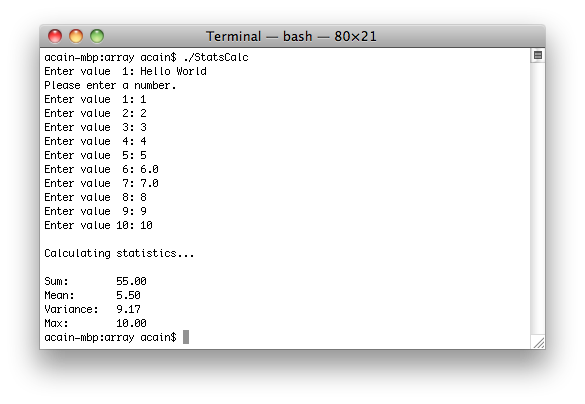
\includegraphics[width=0.6\textwidth]{./topics/arrays/images/SimpleStats} 
   \caption[Statistics Calculator Terminal]{Statistics Calculator run from the Terminal}
   \label{fig:simple-stats}
\end{figure}


\clearpage
\subsection{Array} % (fold)
\label{sub:array}

\begin{figure}[h]
   \centering
   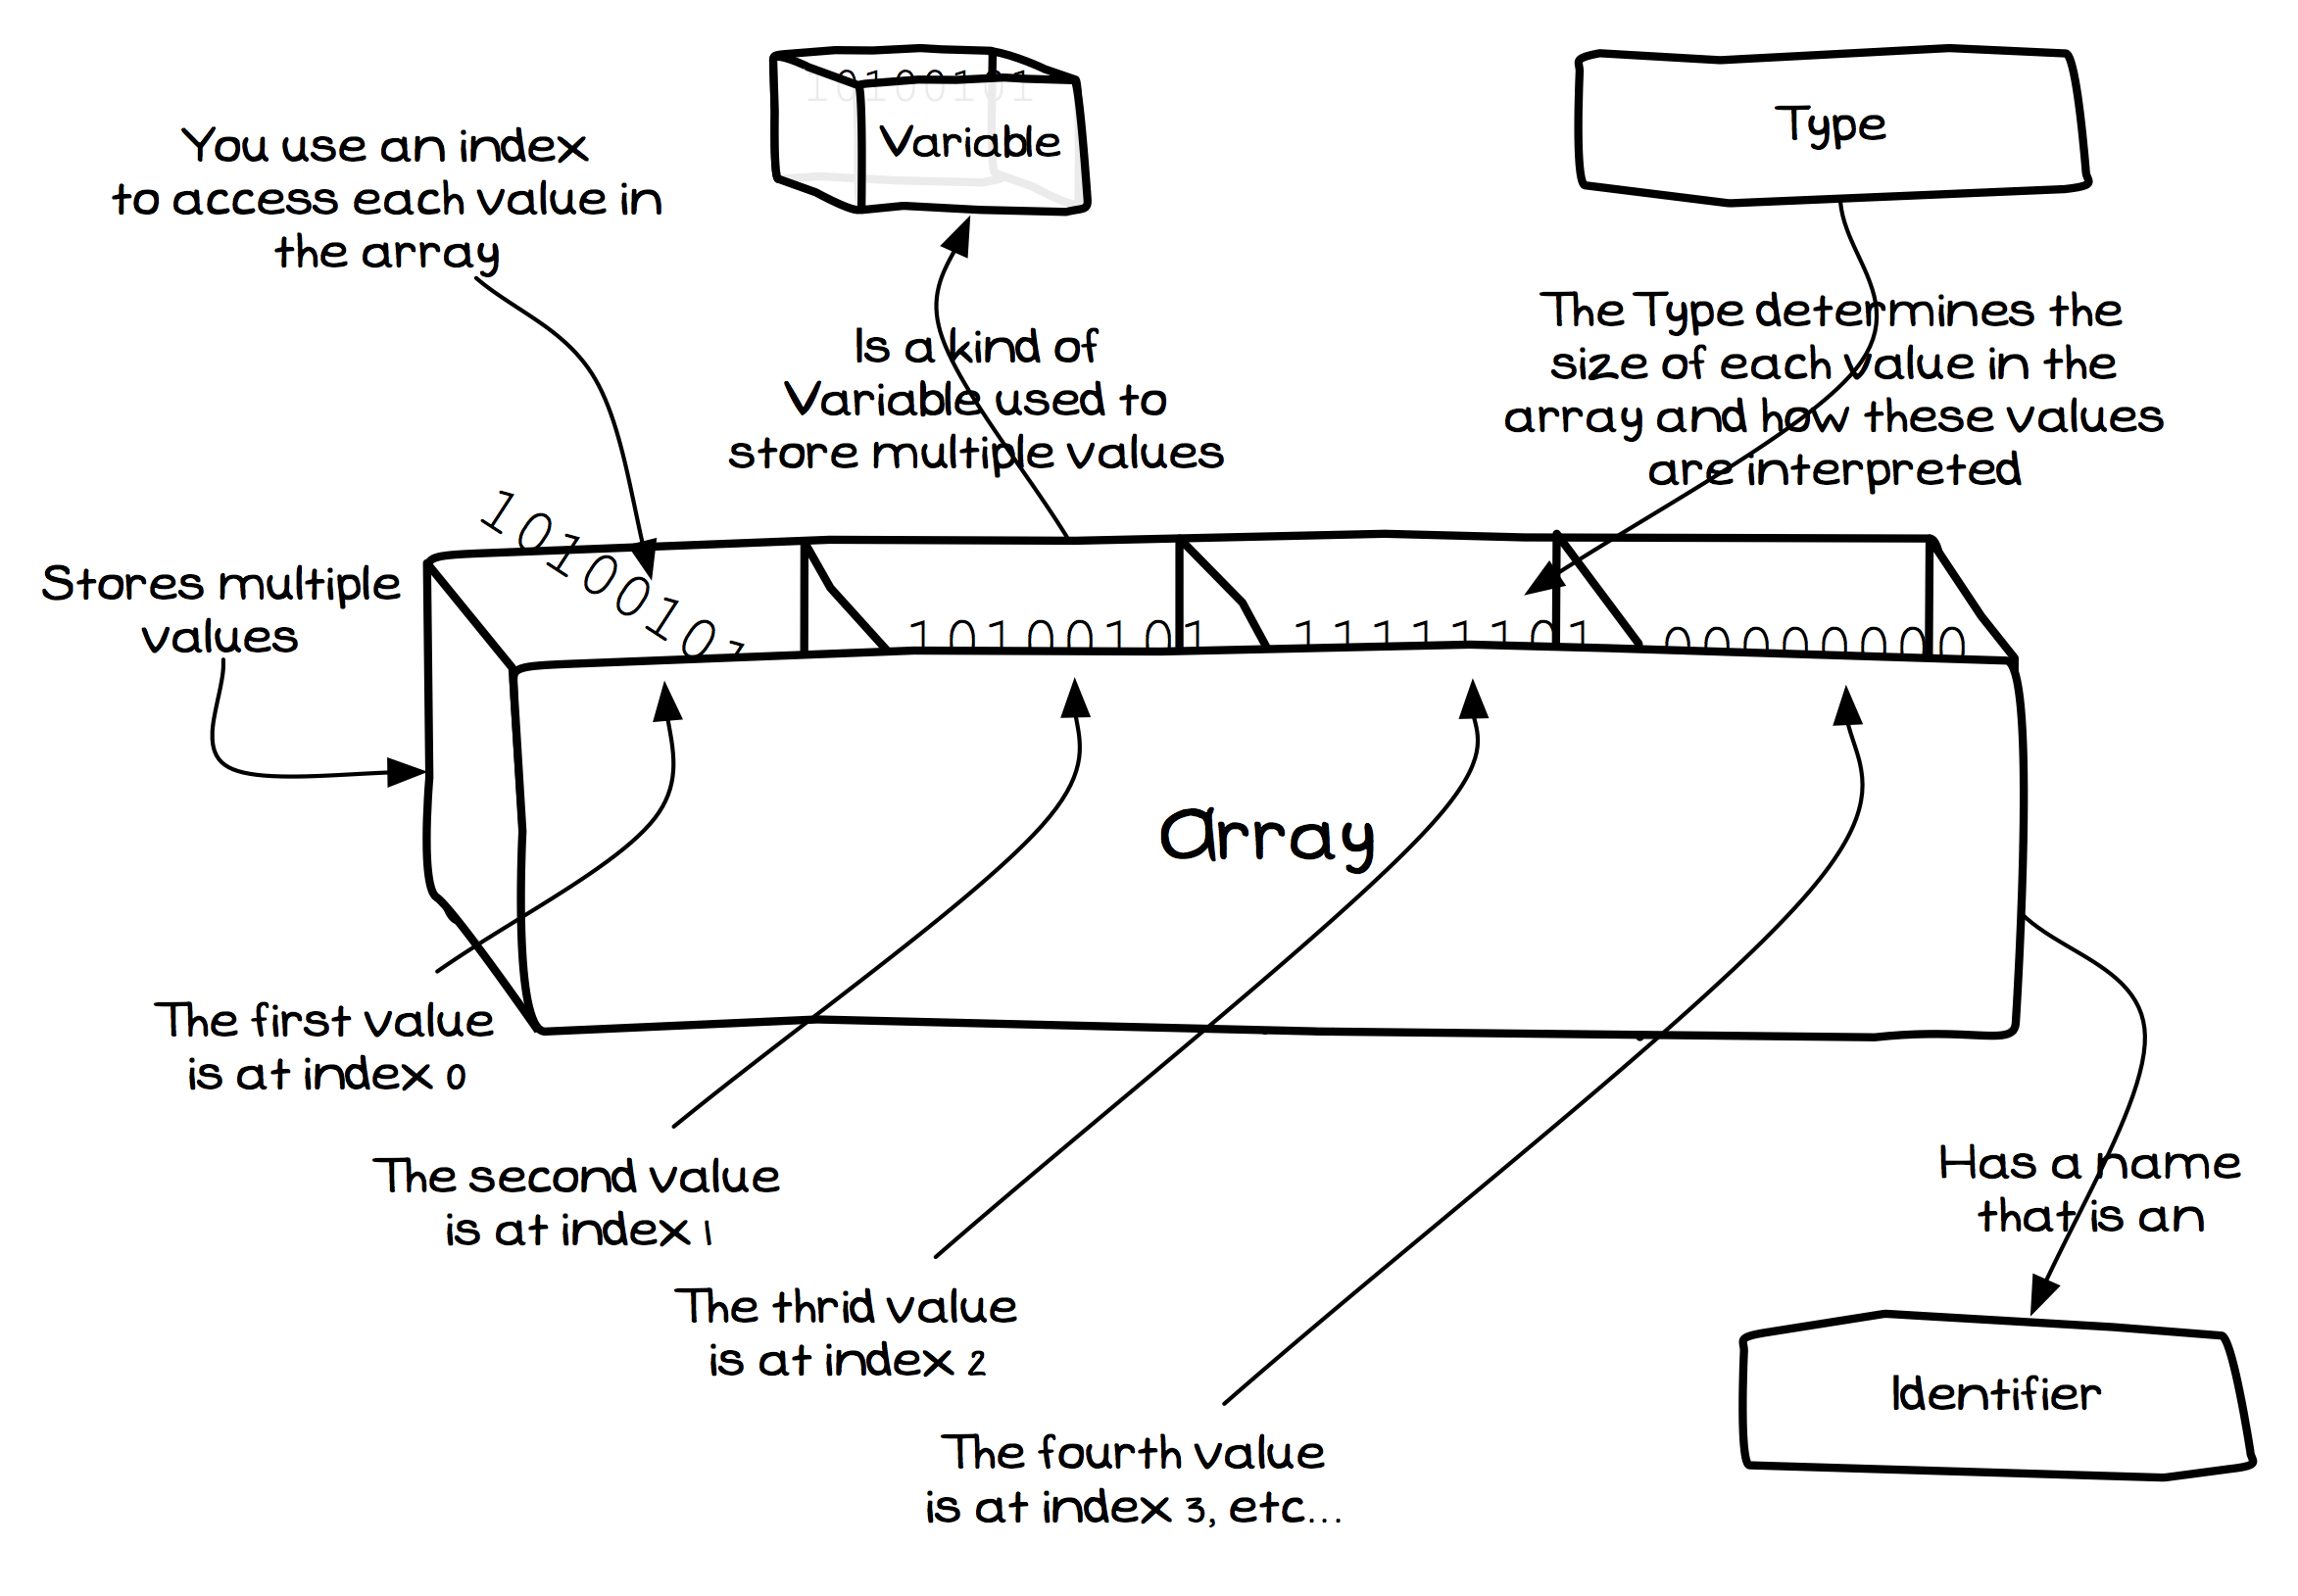
\includegraphics[width=\textwidth]{./topics/arrays/diagrams/Array} 
   \caption{Arrays allow you to store multiple values in a variable}
   \label{fig:type-decl-array}
\end{figure}


% subsection array (end)
\clearpage
\subsection{Assignment Statement (with Arrays)} % (fold)
\label{sub:assignment_statement_with_arrays_}

The assignment statement allows you to store a value in a variable. This can now be extended to allow you to store a value in an element of an array. To achieve this you indicate the array you want to store the value in, as well as the index at which the value is to be stored.

\begin{figure}[h]
   \centering
   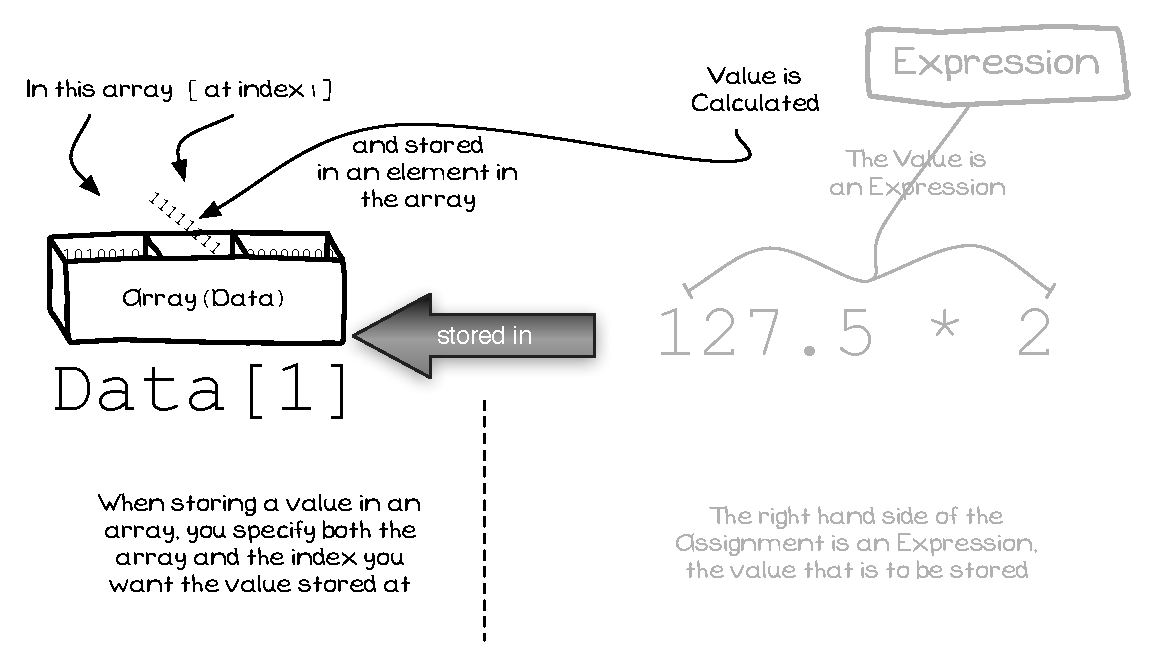
\includegraphics[width=\textwidth]{./topics/arrays/diagrams/AssignmentWithArray} 
   \caption{Arrays allow you to store multiple values in a variable}
   \label{fig:assignment-with-arrays}
\end{figure}

\mynote{
\begin{itemize}
  \item The assignment statement is an \textbf{action}, storing a value in a variable or array.
  \item When working with arrays you specify the array, and index at which to store the value.
  \item This stores a value into an element of an array.
  \item The two snippets below indicate how this is coded in C and Pascal. In each case \texttt{data} is the name of the array variable, and 1 is the index of the second element. The code in the snippet stores a 255 in the second element of the array.
\end{itemize}
}


\csection{In C you can achieve this using: \csnipet{data[1] =  127.5 * 2;}. }

\passection{In Pascal you can achieve this using: \passnipet{data[1] :=  127.5 * 2;}.}

\clearpage
\subsubsection{Assigning all elements of an array} % (fold)
\label{ssub:assigning_all_elements_of_an_array}

Many languages also allow you to copy the entire contents of an array into another array. In these cases each of the elements of one array are copied into the elements of the destination array (left hand side of the assignment).

\begin{figure}[h]
   \centering
   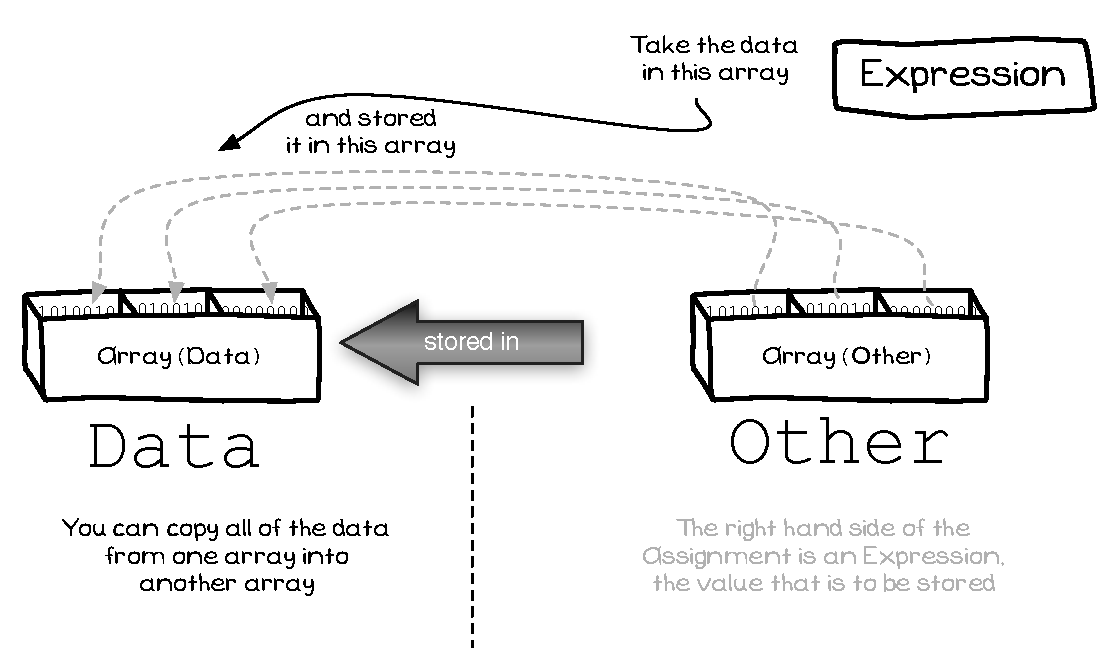
\includegraphics[width=\textwidth]{./topics/arrays/diagrams/AssignmentWithArray2} 
 \caption{All of the elements of an array can be copied across in the assignment statement}
 \label{fig:assignment-with-arrays2}
\end{figure}

\mynote{
\begin{itemize}
  \item The size of the two arrays should match.
  \item The value from each of the elements of the array on the right hand side will be copied into the matching element in the array on the left hand side.
\end{itemize}
}

\csection{This \textbf{cannot} be done in C with an assignment statement, rather it is achieved using the \texttt{memcopy} function. The code for this is as follows, with \texttt{sz} being the number of elements to copy. \csnipet{memcpy(data, source, size_of(double) * sz)}}

\passection{In Pascal you can achieve this using: \passnipet{data := other;}.}

% subsubsection assigning_all_elements_of_an_array (end)

% subsection assignment_statement_with_arrays_ (end)
\clearpage
\subsection{Expressions (with Arrays)} % (fold)
\label{sub:expressions_with_arrays_}

Expressions allow you to read values from the elements of an array. To get an elements value you must supply the name of the array, and the index of the element you want to read.

\begin{figure}[h]
   \centering
   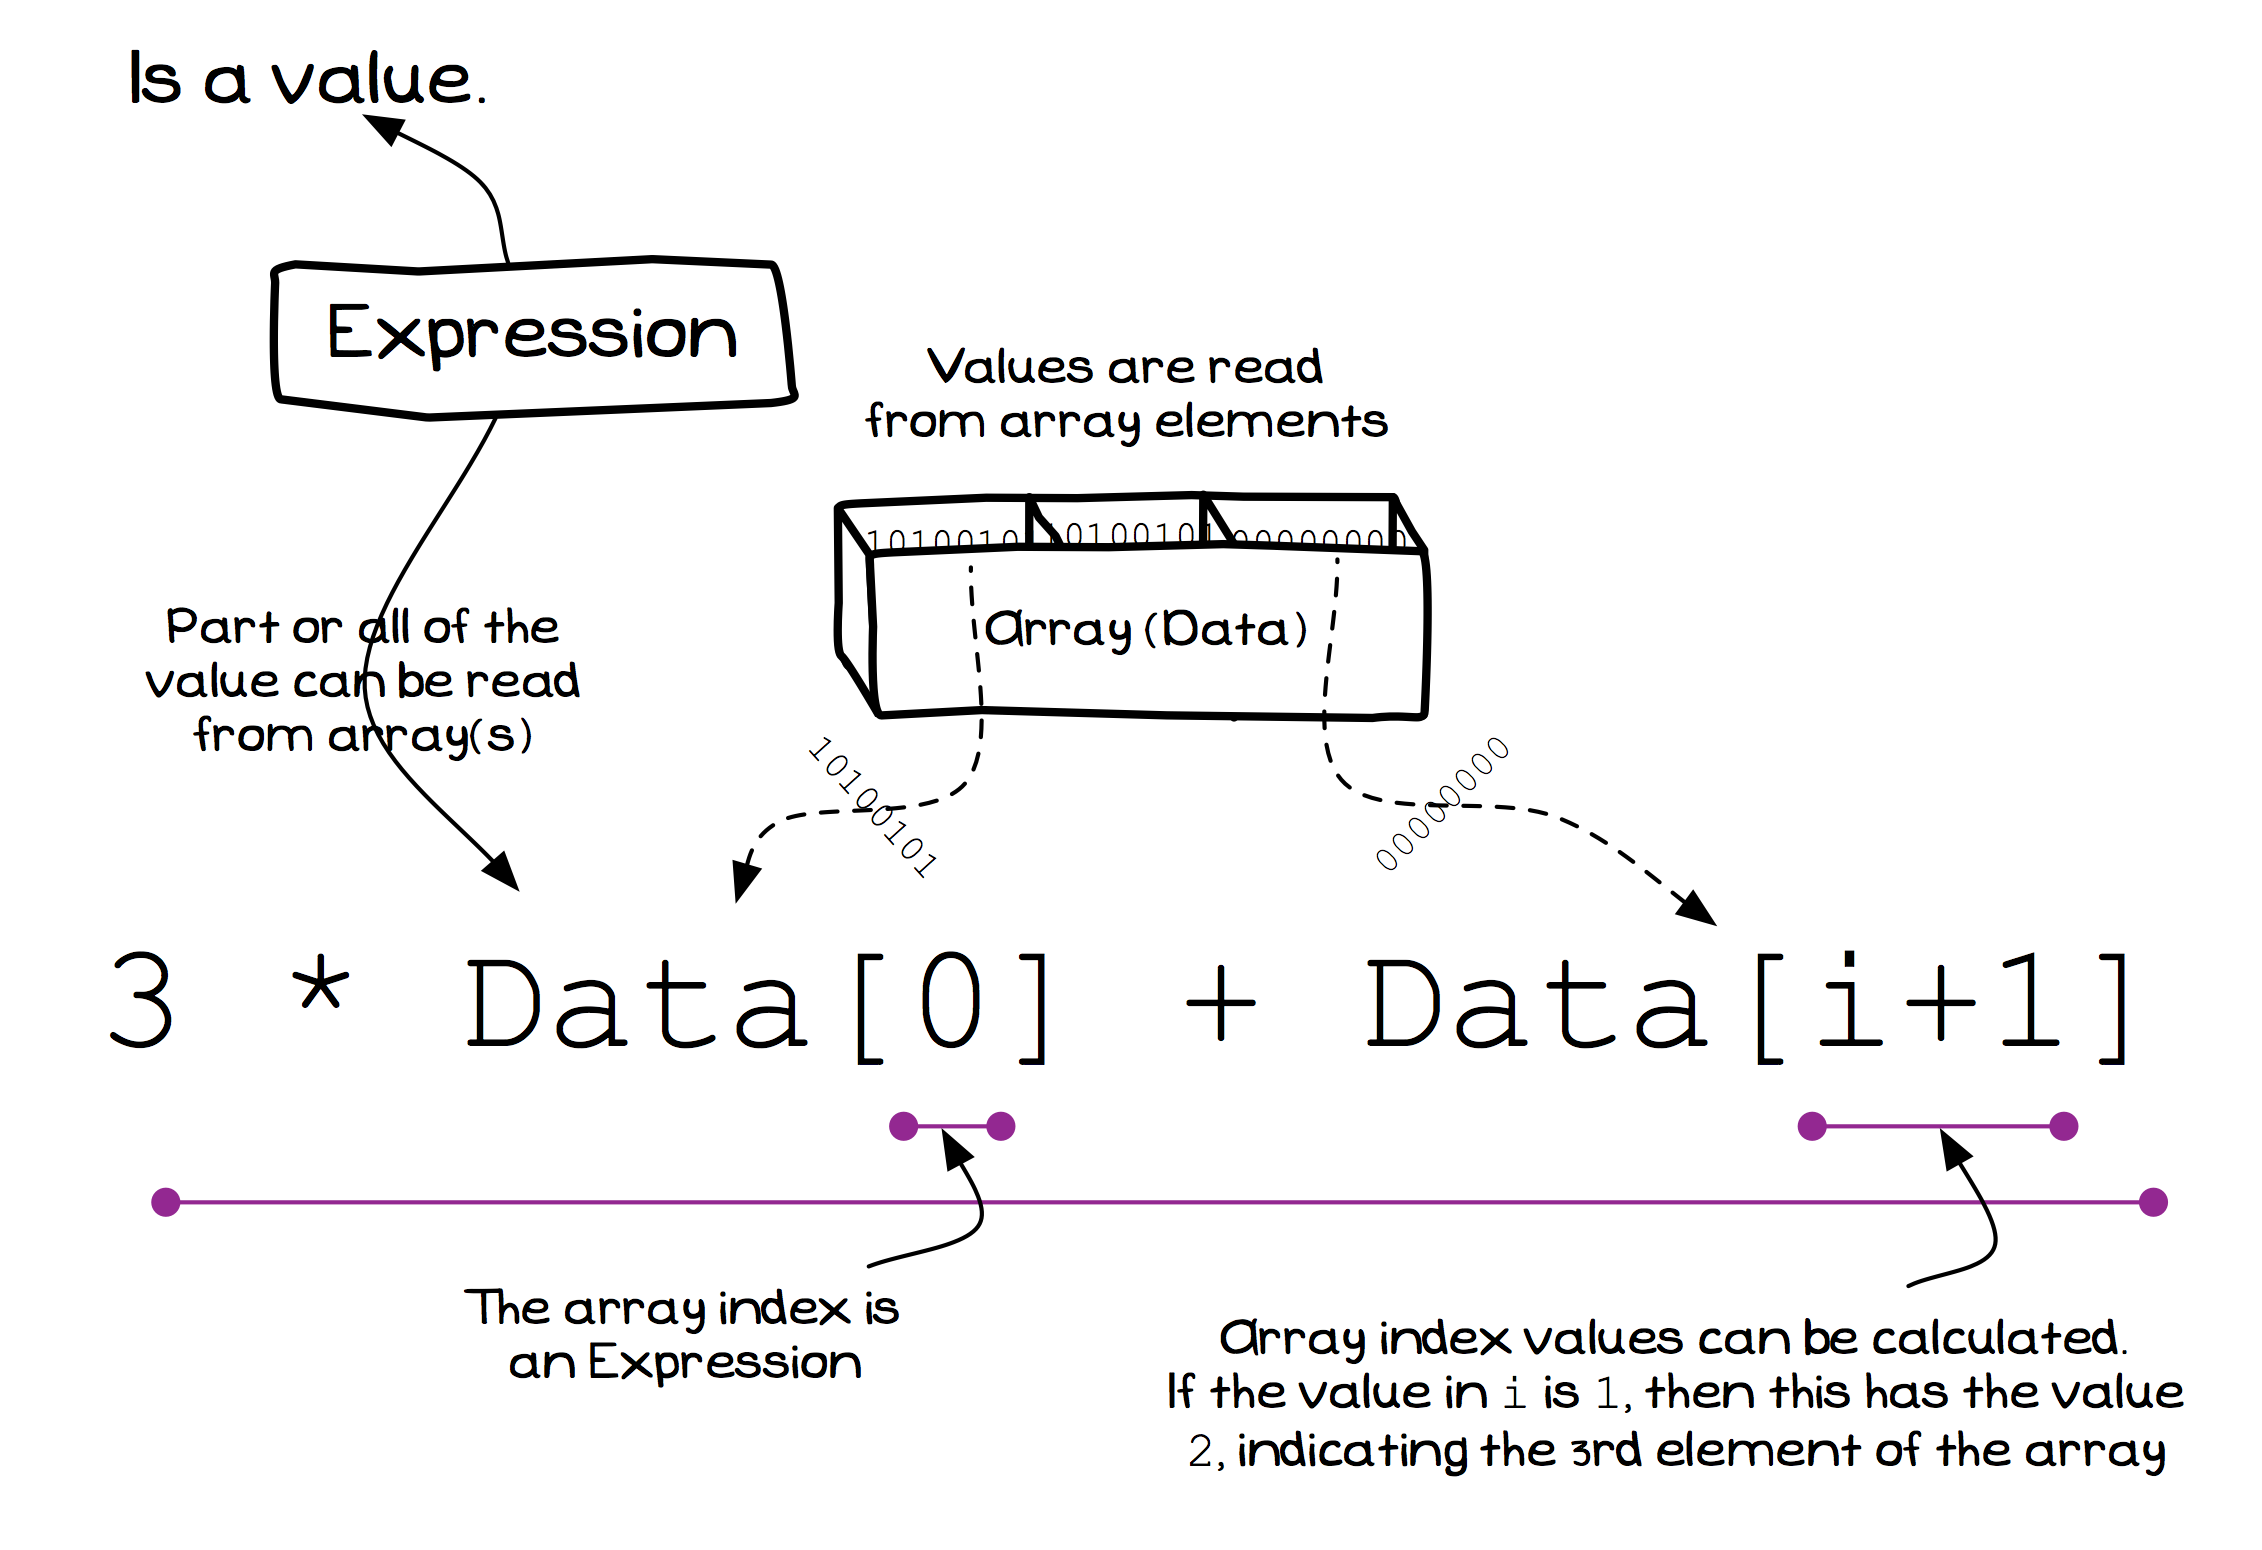
\includegraphics[width=\textwidth]{./topics/arrays/diagrams/ExpressionWithArray} 
   \caption{You can read the values back from an array}
   \label{fig:expression-with-arrays}
\end{figure}

\mynote {
\begin{itemize}
  \item Expression is the \textbf{term} given to the code that calculates values within your Statements.
  \item You can read the values of elements of an array in an expression.
  \item The index values used to access the individual elements of an array are expressions themselves.
  \item Arrays are similar to variables in expressions, the expression reads the value from the element of the array.
  \item The index you supply determine which value is read.
\end{itemize}
}

% subsection expressions_with_arrays_ (end)
\clearpage
\subsection{Pass by Reference} % (fold)
\label{sub:pass_by_reference}

As with other Variables, you can pass an array to Functions and Procedures. The only real difference is that the array can potentially store significantly more data than other variables. When the array is passed by value each of its elements must be passed to the Parameter. Passing the parameter in this way means that there will be two copies of the data in memory, which takes more time and more memory.

You should avoid passing arrays by value, and instead pass them by reference. When passed by reference the array itself is passed across. This gives the called Function or Procedure access to the data, but does not require that the values be copied across.

One issue with always using pass by reference is that it allows the called code to change the data in array you are passing across. This can be useful, but at other times you want to pass the data across without allowing it to be changed by the called code. Both C and Pascal allow you to indicate that the data you are passing should be passed by reference, but that it cannot be changed in the called code.

\begin{figure}[h]
   \centering
   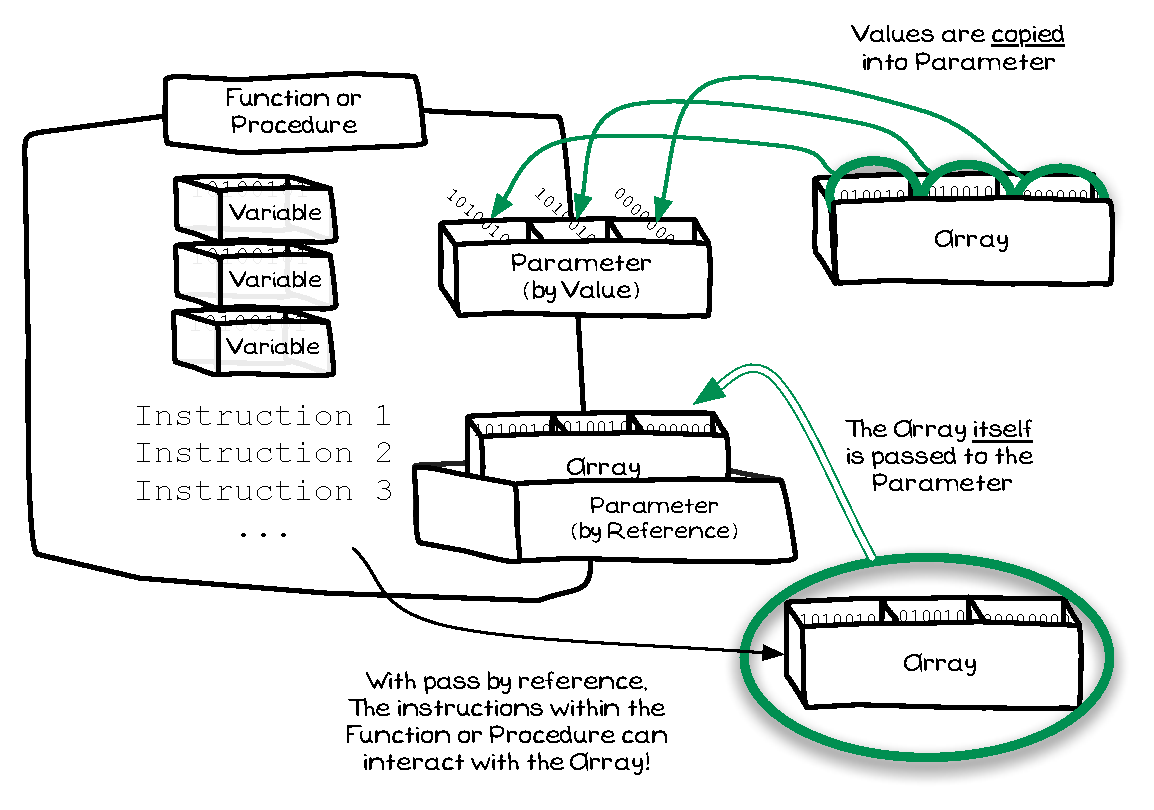
\includegraphics[width=0.9\textwidth]{./topics/arrays/diagrams/ByRefByVal} 
   \caption{Arrays should always be passed by Reference}
   \label{fig:array-by-ref-by-val}
\end{figure}

\mynote{
\begin{itemize}
  \item Pass by Reference and Pass by Value are \textbf{terms} that explain how data is passed to a Parameter.
  \item With arrays you should always use \emph{Pass by Reference}. This will be faster and take less memory.
  \item The \textbf{const} keyword can be used to indicate that the parameter should not be able to be changed by the called code.
\end{itemize}
}

\csection{In C you cannot pass an array by value, instead all arrays are passed by reference automatically by the language.}

% subsection passing_by_reference (end)
\clearpage
\subsection{For Loop} % (fold)
\label{sub:for_loop}

As has been shown in previous chapters, Computers can only perform simple actions. They cannot perform an action on all of the elements in our arrays. For example, a computer cannot sum \textbf{all} of the values in an array. What you need to do is think of these tasks so that they can be performed \textbf{for \emph{each}} value in the array. So the sum would become, for each of the numbers in the array, add the number to a running total. When this has been performed for each element in the array you have the sum of all of the elements.

The for loop is a \nameref{sub:pre_test_loop} that repeats a block of code a number of times. You can think of it like a counting loop, with it counting from a start value to an end value. The for loop has a \textbf{control variable} that has the number of the current loop as its value.

\begin{figure}[h]
   \centering
   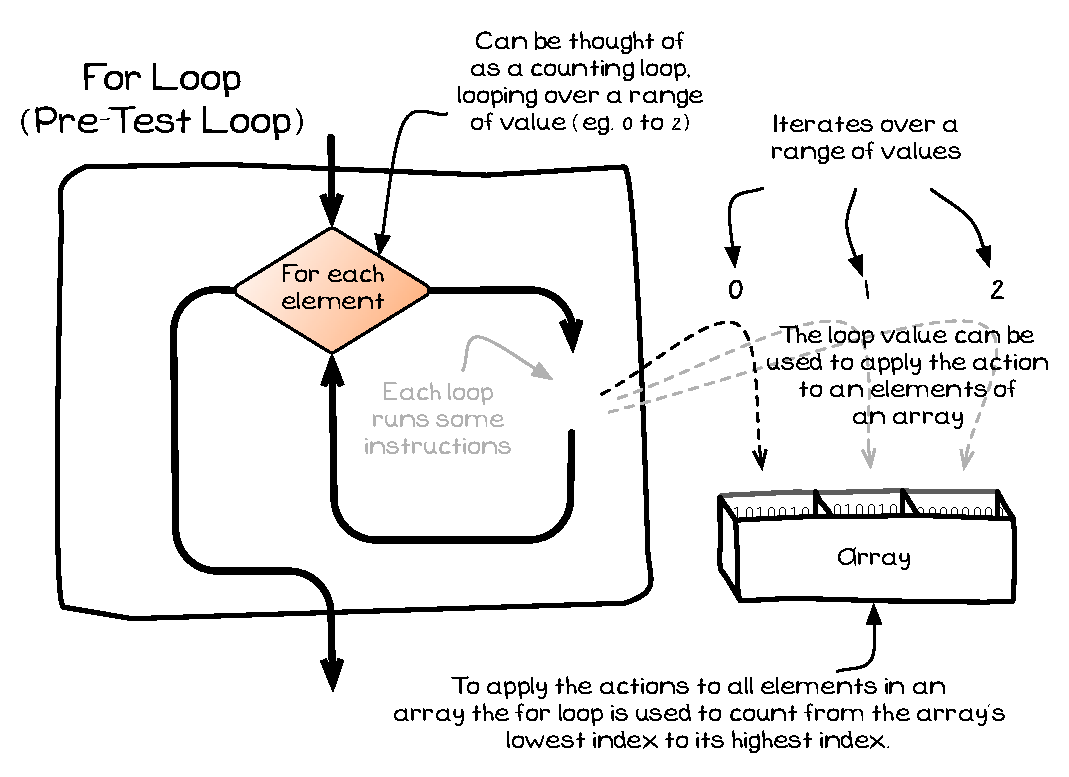
\includegraphics[width=\textwidth]{./topics/arrays/diagrams/For} 
   \caption{The for loop can be used to loop through the elements of an array}
   \label{fig:for-loop}
\end{figure}

\mynote{
\begin{itemize}
  \item A for loop is an \textbf{action}, a kind of statement you can use to command the computer to perform an action.
  \item The key is to think about processing \textbf{each} element in an array, rather than thinking about \emph{all} elements of an array.
  \item The for loop can then provide the infrastructure to repeat this code \emph{for each} element in the array.
  \item The for loop is designed to work well with the array. The values in the \emph{control variable} can be used to access the individual elements of the array.
  \item When processing the elements of an array you have it loop from the lowest index value (0) to the highest index value (n - 1).
\end{itemize}
}

% subsection for_loop (end)
\clearpage
\subsection{String} % (fold)
\label{sub:string}

Textual data is stored as an array of characters. 

\begin{figure}[h]
   \centering
   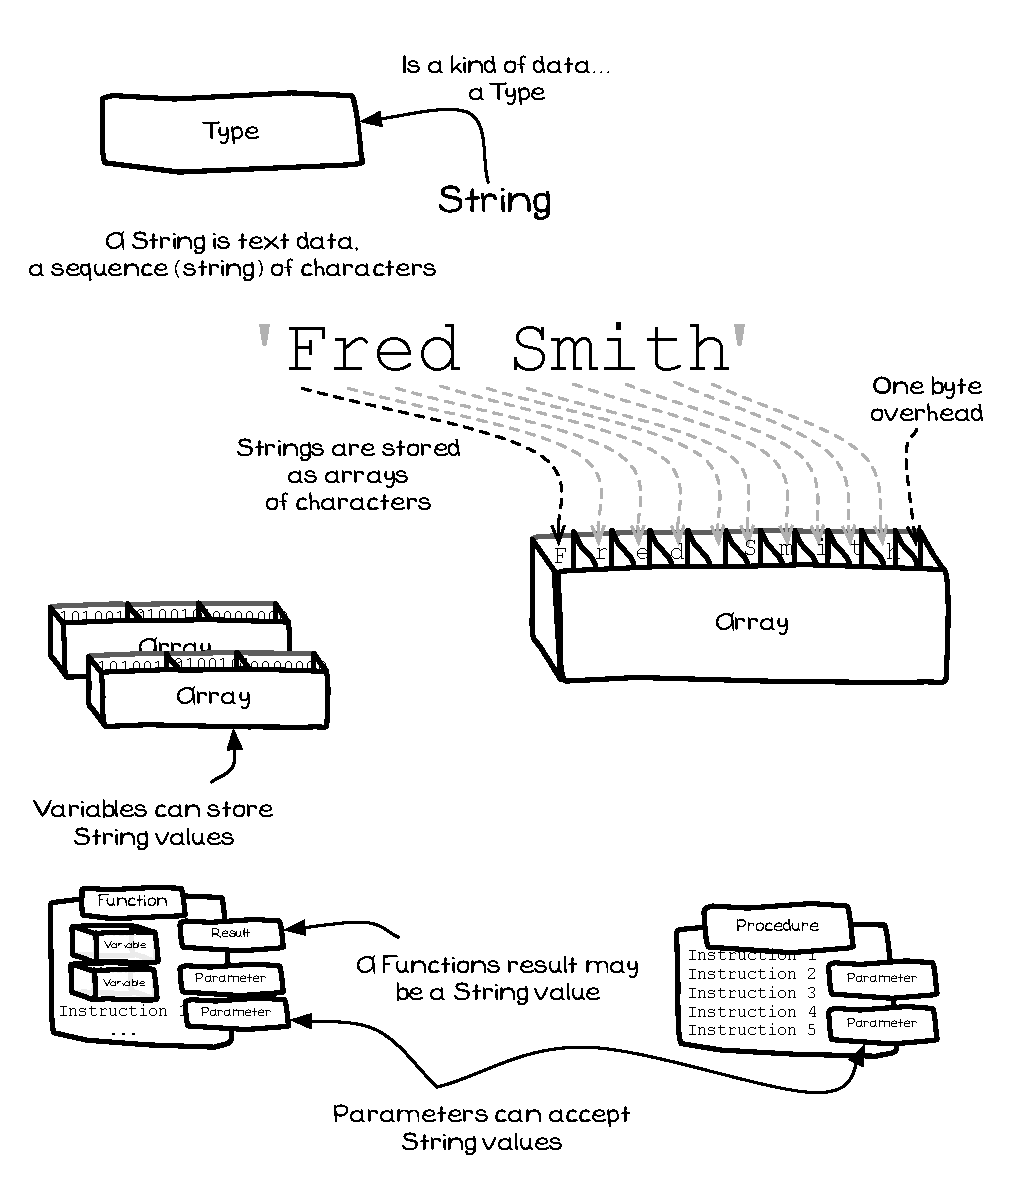
\includegraphics[width=0.8\textwidth]{./topics/arrays/diagrams/String} 
   \caption{Strings are textual data, stores as an array of characters}
   \label{fig:strings}
\end{figure}

\mynote{
\begin{itemize}
  \item Boolean is an existing \textbf{artefact}, it is a \nameref{sub:type} that has been defined to represent text values.
  \item A string is an array of characters.
  \item Both C and Pascal have additional overhead in the string data. In C the overhead is used to store a single terminating character that indicates the end of the string, in Pascal this stores the number of characters.
\end{itemize}
}

\csection{C does not have a native String type, instead you use an array of characters. As a result, C has very limited support for string data. For details see \nameref{sub:c_string}.}

% subsection string_type (end)
\clearpage
\subsection{Summary} % (fold)
\label{sub:arrays_summary}

This Chapter introduced a number of concepts related to working with multiple values in code.

\begin{figure}[h]
   \centering
   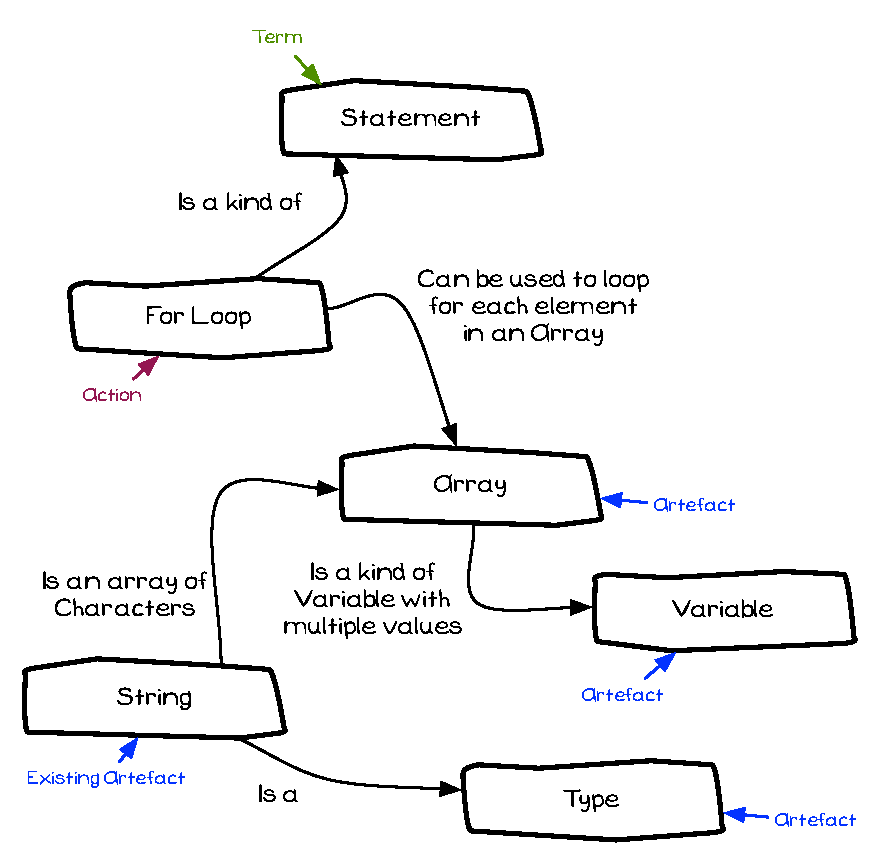
\includegraphics[width=0.8\textwidth]{./topics/arrays/diagrams/Summary} 
   \caption{Concepts covered in this Chapter}
   \label{fig:arrays-summary}
\end{figure}

\mynote{
\begin{itemize}
  \item The central concept of this chapter is the \nameref{sub:array}. An array is a variable that can store multiple values.
  \item When you work with arrays make any logic you want to apply to \emph{all elements} will be coded using \textbf{for each} element and the \nameref{sub:for_loop}.
  \item \nameref{sub:string}s are arrays of characters, and can be used to store textual data in your code.
\end{itemize}
}


% subsection summary (end)


% section data_type_concepts (end)
\clearpage
\section{Using these Concepts} % (fold)
\label{sec:arrays_using_these_concepts}

Arrays make it easier to work with multiple values, allowing you to have a single variable that stores multiple values. With arrays you can start to create programs that process larger quantities of data.

\subsection{Designing Statistics Calculator} % (fold)
\label{sub:designing_statistics_calculator}

\tref{tbl:stats-calc-prog} contains a description of a small statistics programs. This program reads a number of values from the user, and then outputs some statistics calculated from these values. This program will make use of arrays to store the values entered, and then calculate the required statistics.

\begin{table}[h]
\centering
\begin{tabular}{l|p{10cm}}
  \hline
  \multicolumn{2}{c}{\textbf{Program Description}} \\
  \hline
  \textbf{Name} & \emph{Statistics Calculator} \\
  \\
  \textbf{Description} & Reads values from the user and calculates a range of statistics that are output to the Terminal. Statistics output include \textbf{mean}, \textbf{maximum}, \textbf{sum}, and \textbf{variance}.\\
  \hline
\end{tabular}
\caption{Description of the Statistics Calculator program.}
\label{tbl:stats-calc-prog}
\end{table}

As before, the process to design and implement this program will follow a number of steps:
\begin{enumerate}
  \item Understand the problem, and get some ideas on the tasks that need to be performed.
  \item Choose the artefacts we will create and use
  \item Design the control flow for the procedural\footnote{The program, and any Functions and Procedures.} artefacts
  \item Map these artefacts to code
  \item Compile and run the program
\end{enumerate}

% subsection designing_statistics_calculator (end)

\subsection{Understanding the Statistics Calculator} % (fold)
\label{sub:understanding_the_statistics_calculator}

Most of the ideas around the Statistics Calculator should be fairly straight forward. The main thing to be checked if the equation needed to calculate the different statistics, and then to convert these into steps for the computer.

\subsubsection{Calculating Sum} % (fold)
\label{ssub:calculating_sum}

The \textbf{sum} is the simplest of the Statistics to calculate. This involves adding together all of the numbers in the array. The main issue here is that the computer cannot add all of these values together, and we must rethink our logic to express it in terms of processing \emph{for each} element.

Think about the way you would sum a list of numbers, this is now the task you need to code for the Computer. What is it that you do with each number? To think this through write a list of random numbers down, and then calculate the sum. Do it slowly, and think about the tasks that you are performing \emph{for each number}.

You should have noticed that you are keeping a running total, and that you add the value of each number from the list to that. When you have done this for each number in the list you have the total. The Pseudocode for this is shown in \lref{plst:sum}.

\pseudocode{plst:sum}{Pseudocode for Sum}{topics/arrays/application/Sum.txt}

\csection{\ccode{clst:sum}{C code for Sum Function. You can read the for loop as \emph{`i starts at 0; while i is less than size; increment i at the end of the loop'}}{topics/arrays/application/sum.c}}

\passection{\pascode{paslst:sum}{Pascal code for Sum Function}{topics/arrays/application/Sum.pas}}

There are three key things to notice about the Pseudocode in \lref{plst:sum}. Firstly the \nameref{sub:for_loop} is used to repeat the loop once for each element in the array. Second, the \texttt{i} variable moves through the valid indexes for the array. Finally, the total is used to keep the running total throughout the code.

The for loop in \nameref{sub:for_loop} will repeat its body once for each value in the array. The \texttt{i} variable will be updated to have the \emph{current} index value each time the loop is repeated. Within the loop the $i^{th}$ value from the array is accessed. This is how the for loop processes each of the values from the array.

The \texttt{total} value keeps track of the current running total. Before the loop its value is set to 0, ensuring that it is appropriately initialised. In the body of the loop the current ($i^{th}$) value of the array is added to the \texttt{total}, and the result stored back into \texttt{total}. This means that by the end of the loop the \texttt{total} variable is now storing the sum of all of the elements of the array.

C and Pascal differ in the amount of support they have for working with arrays. C has very limited support, meaning that you need to do some extra work. Pascal has more build in support for arrays, making some common tasks easier to achieve. The main difference is that C does not keep track of the length of an array. This means that you need to pass the number of elements in the array along with the array to functions and procedures that will work with this data. Pascal, on the other hand, does keep track of the length of arrays and gives you three functions you can use to manage this: \texttt{Low} returns the first index of the array, \texttt{High} returns the last index of the array, \texttt{Length} returns the number of elements in the array.

\csection{The C code for the \texttt{Sum} function is in \lref{clst:sum}. Notice how the \texttt{size} parameter is being used to represent the number of elements in the array. This loop is the standard pattern used to code \nameref{sub:for_loop}s that loop over elements in an array in C.}

\passection{The Pascal code for the \texttt{Sum} function is in \lref{paslst:sum}. Notice how it is using the \texttt{Low} and \texttt{High} functions to get the range of valid array indexes. This loop is the standard pattern used to code \nameref{sub:for_loop}s that loop over elements in an array in Pascal.}

% subsubsection calculating_sum (end)

\clearpage
\subsubsection{Calculating Mean} % (fold)
\label{ssub:calculating_mean}

The mean of a list of values is the sum of those values divided by the number of values. In the case of the Statistics Calculator program there is already a \texttt{Sum} function, so the \texttt{Mean} function does not need to recalculate the sum, it can just call the \texttt{Sum} and use the result returned.

The length of the array can be calculated in Pascal using its \texttt{Length} function, where as C can use the \texttt{size} parameter to determine the number of elements in the array. In both cases the basic logic is the same, you use the \texttt{Sum} function to calculate the sum and then divide this by the number of elements in the array.

\pseudocode{plst:mean}{Pseudocode for Mean}{topics/arrays/application/Mean.txt}

\csection{\ccode{clst:mean}{C code for Mean Function}{topics/arrays/application/mean.c}}

\passection{\pascode{paslst:mean}{Pascal code for Mean Function}{topics/arrays/application/Mean.pas}}

% subsubsection calculating_mean (end)

\clearpage
\subsubsection{Calculating Maximum} % (fold)
\label{ssub:calculating_maximum}

Calculating the largest value in the array, the maximum, will require the logic be adjusted to use the \emph{for each} style. How do you calculate the largest value in a list of numbers? With a small list you are likely to just quickly scan it and see the largest value. Think about the tasks you need to perform, and maybe think about how you would do it for a very long list of numbers, one that spans across many pages.

The algorithm needed to find the maximum value in an array needs to perform an action \emph{for each} element of the array. It needs to process each value in isolation, ignoring the other values from the list.

The key is similar to the logic from the \texttt{Sum} function. You need to keep a \emph{running} maximum. This will store the \emph{current} maximum from the array as you loop through \emph{each element} of the array. Like the sum this value can be updated within the loop.

The Pseudocode for this is in \lref{plst:max}. Notice that its basic layout if the same as the \texttt{Sum} function in \lref{plst:sum}. It initialises the \texttt{max} value and then loops through the array performing an action for each value. In this case the action is to check if the $i^{th}$ value of the array is larger than the running maximum in the \texttt{max} variable. When this is the case a new maximum has been found and is stored in the \texttt{max} variable.

One of the important differences between \texttt{Maximum} and \texttt{Sum} is the initialisation of the \texttt{max} value. In \texttt{Maximum} this cannot be initialised to 0 as this would fail to find the maximum if all values were negative. The maximum must be a value from the array, so it is initialised to the first value in the array. The for loop will then start looping from the $2^{nd}$ element, as the $1^{st}$ has already been processed.

\pseudocode{plst:max}{Pseudocode for Maximum}{topics/arrays/application/Max.txt}

% \csection{\ccode{clst:max}{C code for Maximum Function}{topics/arrays/application/max.c}}
% 
% \passection{\pascode{paslst:max}{Pascal code for Maximum Function}{topics/arrays/application/Max.pas}}

% subsubsection calculating_maximum (end)

\clearpage
\subsubsection{Calculating Variance} % (fold)
\label{ssub:calculating_variance}

The last statistic to calculate is the Variance. The processing for this will be very similar to the \texttt{Sum} and \texttt{Maximum} functions, though the actual calculation is a little more complex. \eref{eq:var} shows how the Variance of a sample is calculated.

\begin{equation}
  \label{eq:var}
  var(x) = \frac{\displaystyle \sum_{i=1}^{n}(x_{i} - \overline{x})^2}{n - 1}
\end{equation}

In \eref{eq:var} $x$ is the array being processed, $\overline{x}$ is the mean of $x$, $x_i$ is the value of the $i^{th}$ element of $x$, and $n$ is the number of elements in the array. The Sigma indicates that $x_{i} - \overline{x}$ needs to be summed for each element of $x$.

The steps to calculate the Variance are therefore:
\begin{enumerate}
  \item Determine the value of the mean ($\overline{x}$).
  \item Calculate $(x_{i} - \overline{x})^2$ for each element, and store these in a running sum (called \texttt{temp}).
  \item Divide the value (from \texttt{temp}) by the number of elements in the array minus one.
\end{enumerate}

The matching Pseudocode for this is shown in \lref{plst:variance}. In this case $x$ is the \texttt{data} array. In Step 1 the mean ($\overline{x}$) is calculated once and stored in \texttt{avg}. The loop starts at Step 3, and runs \emph{for each} element of the array. The value $(x_{i} - \overline{x})^2$ is calculated for each element in Step 4, and added to the running total stored in \texttt{temp}. The final result is then calculated and the result returned in Step 5.

\pseudocode{plst:variance}{Pseudocode for Variance}{topics/arrays/application/Variance.txt}

% subsubsection calculating_variance (end)

% subsection understanding_the_statistics_calculator (end)

\clearpage
\subsection{Choosing Artefacts for Statistics Calculator} % (fold)
\label{sub:choosing_artefacts_for_statistics_calculator}

In understanding these concepts we have uncovered some Functions that will be included in the program's design. 

With the calculations thought through the design seems to be coming together. So far we have thought through the steps needed to calculate the output, but we have not thought about how these values will be read into the program.

Programs can be thought of as transforming data, taking inputs and generating outputs, as shown in \fref{fig:input-output-overview}. So far we have examined the processing needed to create the outputs, but we still need to consider how the data gets into the program, the inputs.

\begin{figure}[h]
   \centering
   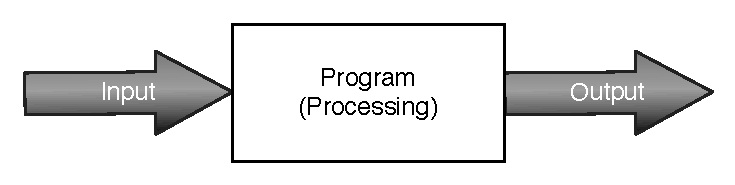
\includegraphics[width=0.6\textwidth]{./topics/arrays/diagrams/ProcessingOverview} 
   \caption{Programs convert Inputs to Outputs}
   \label{fig:input-output-overview}
\end{figure}

At the start of the program the user will need to enter the values that will be stored in the array. This task can be coded in a \texttt{Populate Array} procedure. This will get the user to enter all of the values into the array. In other words it will allow the user to enter \emph{each value} in the array.

The logic for populating the array can be split into a \texttt{Populate Array} procedure that calls a \texttt{Read Double} function. The \texttt{Read Double} function will be very useful across a number of different programs, so this may be able to be used elsewhere.

\subsubsection{Reading double values from the user} % (fold)
\label{ssub:reading_double_values_from_the_user}

\fref{fig:read-double-flow} shows the flowchart for the process of reading a double value from the user. This includes a \nameref{sub:pre_test_loop} that repeatedly asks the user to enter a number if they value they enter is not a number. This demonstrates a standard \emph{validation} loop, in which you read a value, and check that it is valid in a loop. 

The C and Pascal code for this are both slightly different to the flowchart due to different way they handle input and the features they offer to for converting the value read to a number. Details of these are shown alongside \lref{clst:read_double} and \lref{paslst:read_double}.

\begin{figure}[htbp]
   \centering
   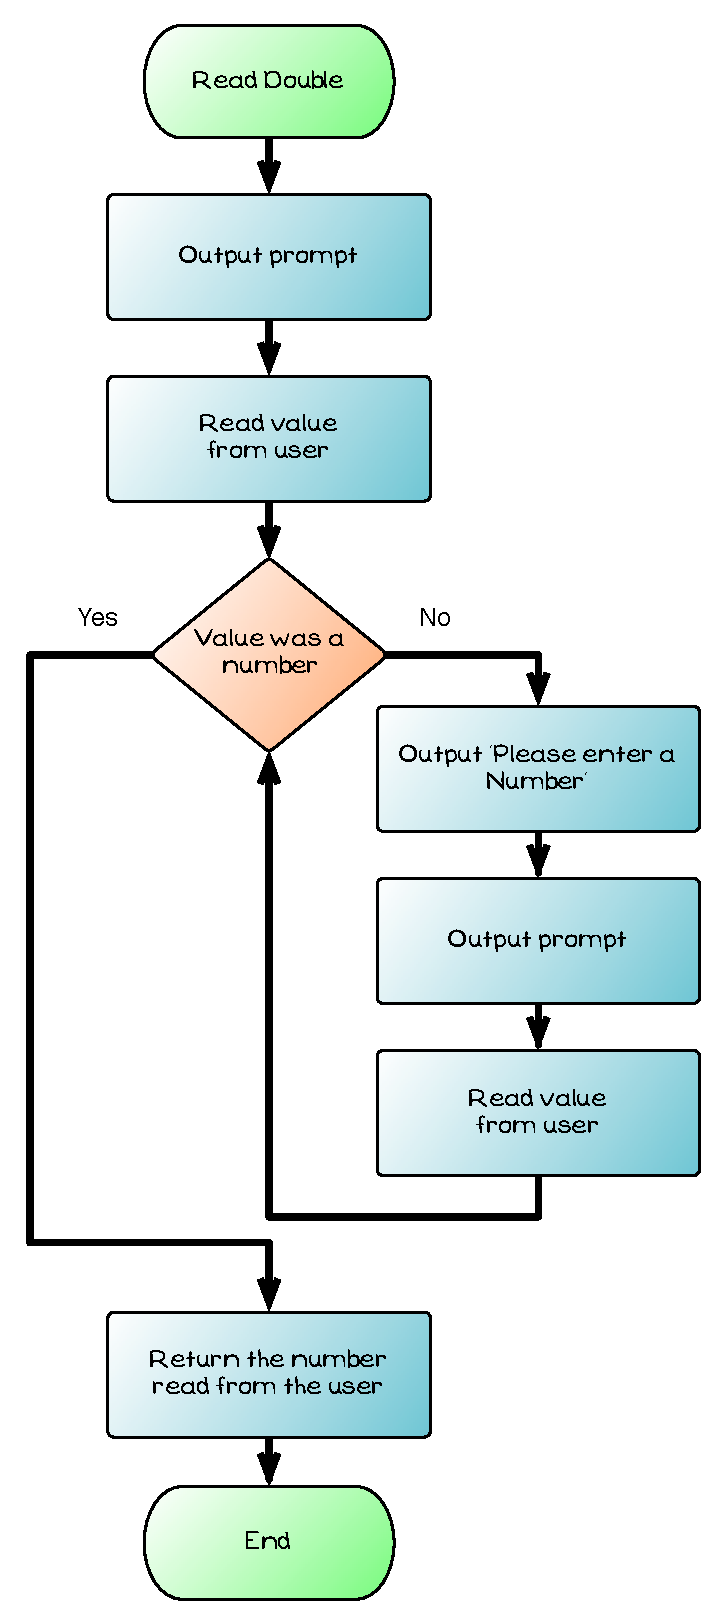
\includegraphics[width=0.45\textwidth]{./topics/arrays/diagrams/ReadDouble} 
   \caption{Flowchart showing the process for reading a double}
   \label{fig:read-double-flow}
\end{figure}

\csection{The C version of \texttt{Read Double}, shown in \lref{clst:read_double}, uses \texttt{scanf} (see \nameref{sub:c_terminal_input}) to read and format the number in the one action. The \texttt{scanf} Function returns a value indicating the number of conversions that were successful. This can be checked in the loop, and the loop is repeated \emph{while} \texttt{scanf} did not convert one value.
\newline\newline
In the loop itself the \texttt{scanf} is used to read past the value that is not a number, as \texttt{scanf} does not proceed when it finds an error. The format string in \texttt{scanf} indicates that it should read everything up to the end of the line.
\ccode{clst:read_double}{C code for \texttt{Read Double}}{topics/arrays/application/read-double.c}}

\passection{The Pascal version of \texttt{Read Double}, shown in \lref{paslst:read_double}, reads the input as a string and then try to convert it to a double. The \texttt{TryStrToInt} Function attempts to convert the text read into a number, storing the value in the \emph{result} variable.
\pascode{paslst:read_double}{Pascal code for \texttt{Read Double}}{topics/arrays/application/ReadDouble.pas}}

% subsubsection reading_double_values_from_the_user (end)

\clearpage
\subsubsection{Populating the Array} % (fold)
\label{ssub:populating_the_array}

With the logic for \texttt{Read Double} in place the next step is to determine the steps needed in the \texttt{Populate Array} procedure. This procedure will loop and read a value from the user for each element of the array. This can use the \texttt{Read Double} function to get the value from the user, and then store this in the array's elements.

A flowchart illustrating the steps in \texttt{Populate Array} is shown in \fref{fig:populate-array-flow}. The decision node is being used to show the control mechanism of the for loop, counting from the lowest index of the array to the highest index. Within the body of the loop the two instructions build a prompt string, and then use this in the call to \texttt{Read Double}. The result returned from \texttt{Read Double} is stored in the current ($i^{th}$) element of the array.

Once again the C and Pascal code differ in how this is implemented, centred on how the \emph{prompt} is built within the loop. Pascal has built in support for Strings, so its code is much simpler. The C code for this requires you to coordinate the steps needed to build the text for the prompt. The details for these are shown in the text accompanying \lref{clst:populate_array} and \lref{paslst:populate_array}.

\begin{figure}[htbp]
   \centering
   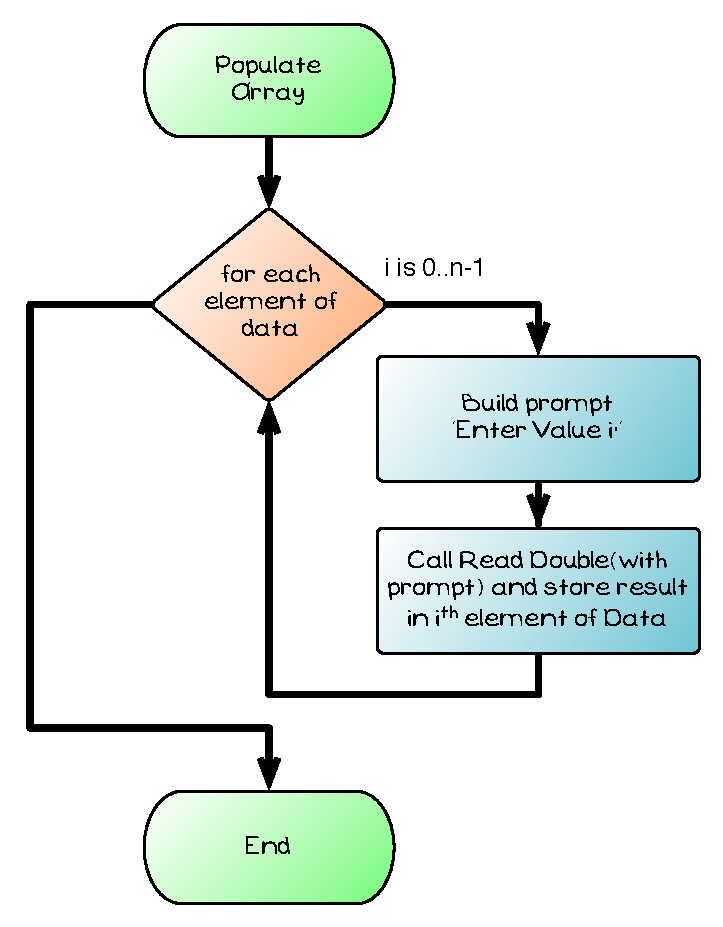
\includegraphics[width=0.6\textwidth]{./topics/arrays/diagrams/PopulateArray} 
   \caption{Flowchart showing the process for \texttt{Populate Array}}
   \label{fig:populate-array-flow}
\end{figure}

\begin{figure}[htbp]
\csection{The C version of \texttt{Populate Array} is shown in \lref{clst:populate_array}. This uses the following functions from \texttt{strings.h}. As C does not know the length of the string each of these functions takes a number (\texttt{n}) that indicates the maximum number of characters to copy.
\begin{itemize}
  \item \texttt{\textbf{strncpy}}: String Copy (n characters). The first parameter is the destination, the second the source, the third is the number of characters.
  \item \texttt{\textbf{sprintf}}: Same as \texttt{printf} (see \nameref{sub:c_console_output}), except that the output is stored in a c-string. In this case the \csnipet{"\% 100"} ensures that only 2 characters (plus the terminator) are written into the string. See \sref{sub:c_string} \nameref{sub:c_string}.
  \item \textbf{\texttt{strncat}}: String Concatenate (n characters). Adds the text in parameter 2 to the end of the string in parameter 1. 
\end{itemize}

\ccode{clst:populate_array}{C code for \texttt{Populate Array}}{topics/arrays/application/populate-array.c}}  
\end{figure}

\begin{figure}[htbp]
  \passection{The Pascal version of \texttt{Populate Array} is shown in \lref{paslst:populate_array}. This uses Pascal's \textbf{\texttt{IntToStr}} function to convert the value \texttt{i + 1} from Integer to String.
  \pascode{paslst:populate_array}{Pascal code for \texttt{Populate Array}}{topics/arrays/application/PopulateArray.pas}}  
\end{figure}

% subsubsection populating_the_array (end)

\subsubsection{Where is the data stored} % (fold)
\label{ssub:where_is_the_data_stored}

The last question to remain is where will the data be stored. The array is a kind of variable, and therefore the array could be a \nameref{sub:local_variable} or a \nameref{sub:global_variable}. As Global Variables should be avoided where possible, this will be coded as a \textbf{Local Variable} within the program's \texttt{Main} procedure. It can then be passed from there to the other Functions and Procedures in the code.

% subsubsection where_is_the_data_stored (end)

\clearpage
\subsubsection{Overview of Statistics Calculator's design} % (fold)
\label{ssub:overview_of_statistics_calculators_design}

That completes the logic needed to implement the Statistics Calculator Program. The final structure is shown in \fref{fig:stats-calc-struct} as a Structure Chart. Notice the double headed arrow on \texttt{data} in the call from \texttt{Main} to \texttt{Populate Array}. This indicates that the data parameter is passing the values into, and getting values out of the \texttt{Populate Array} procedure. Also see how the \texttt{data} value is passed out of \texttt{Main} to the functions that calculate the statistics.

\begin{figure}[htbp]
   \centering
   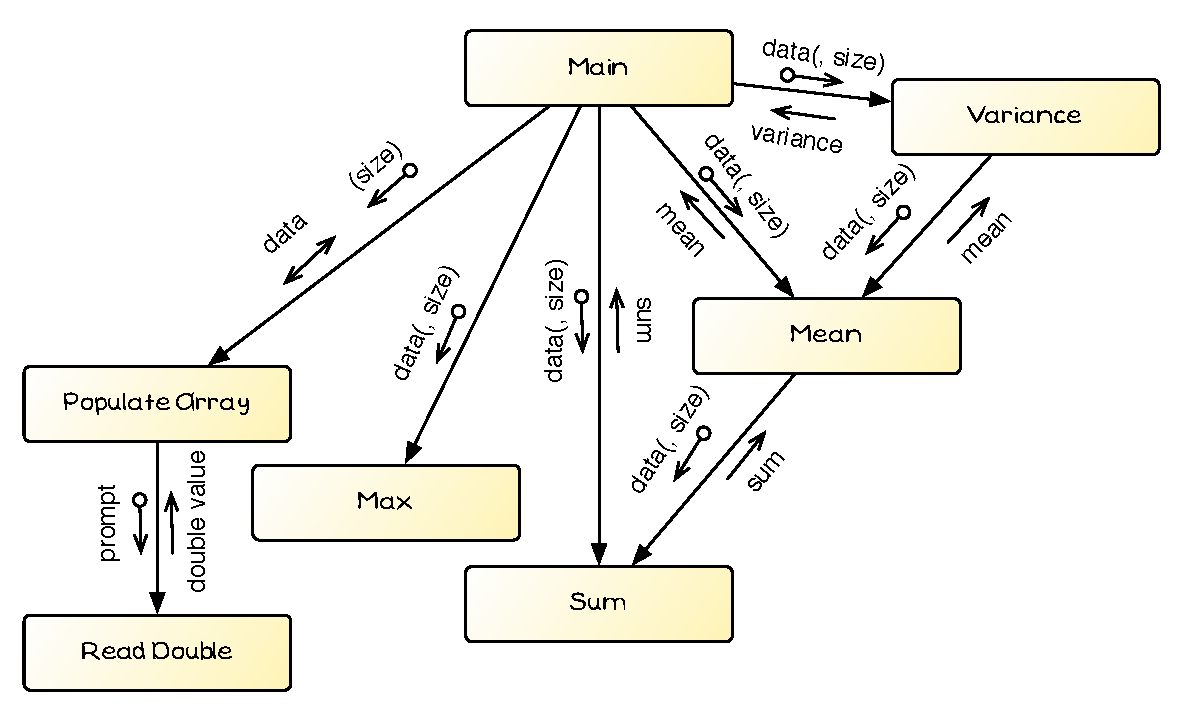
\includegraphics[width=\textwidth]{./topics/arrays/diagrams/StatsCalcStruct} 
   \caption{Structure Chart showing the structure of the \texttt{Statistics Calculator} program}
   \label{fig:stats-calc-struct}
\end{figure}

\mynote{
\begin{itemize}
  \item Remember anytime you need to do something with all of the elements in an array you need to work out how you can achieve this \textbf{for each} element in the array.
  \item Notice that the processing of individual value from the arrays are always similar.
  \item Make sure you can see how the for loop is able to perform these values for each element of the array.
\end{itemize}
}

% subsubsection overview_of_statistics_calculators_design (end)
% subsection choosing_artefacts_for_statistics_calculator (end)

\subsection{Writing the Code for Statistics Calculator} % (fold)
\label{sub:writing_the_code_for_statistics_calculator}

The flowcharts and Pseudocode shown communicate the logic that needs to be coded into the Functions and Procedures of this program. The following two sections, \sref{sec:arrays_in_c} \nameref{sec:arrays_in_c} and  \sref{sec:arrays_in_pascal} \nameref{sec:arrays_in_pascal}, contain a description of the syntax needed to code arrays in the C and Pascal programming languages. This information can be used to write the code for the Statistics Calculator, and other programs.

% subsection writing_the_code_for_statistics_calculator (end)
\clearpage
\subsection{Compiling and Running Statistics Calculator} % (fold)
\label{sub:compiling_and_running_statistics_calculator}

When the code is finished you can compile and run the program. It is a good idea to implement the solution a little bit at a time, compiling and running it frequently as you progress. Try implementing the solution using the following smaller steps, and the tests shown for each.

\begin{enumerate}
  \item Start by getting \texttt{Read Double} to work. In \texttt{Main} just read a single value and output it to the Terminal. \textbf{Tests}:
  \begin{itemize}
    \item Check that a number can be read correctly.
    \item Try entering text, and check the error message is shown and that you can enter a number the next time.
    \item Try entering multiple text values on a single line.
    \item Try entering multiple text values, one after the other.
  \end{itemize}
  \item Implement \texttt{Populate Array}. Include an array in \texttt{Main}, and have its values read in by \texttt{Populate Array}. Print the values back to the Terminal so that you can check this code is working. \textbf{Tests}:
  \begin{itemize}
    \item Enter each of the values and check they are printed out correctly.
    \item Try entering text, this should be handled by \texttt{Read Double} but check it is working correctly with \texttt{Populate Array}.
  \end{itemize}
  \item Implement the \texttt{Sum} Function.
  \textbf{Tests}:
  \begin{itemize}
    \item Test that it works with some basic values.
    \item Try all negative values.
    \item Try a mix of positive and negative values.
  \end{itemize}
  \item Implement the \texttt{Mean} Function. Same tests as \texttt{Sum}.
  \item Implement the \texttt{Variance} Function. Same tests as \texttt{Sum}.
  \item Finish by implementing the \texttt{Maximum} Function. Same tests as \texttt{Sum}.
\end{enumerate}

By building the code a little at a time, and running tests as you go, you will have less code to search when you do find an issue. This makes it easier to fix those little errors that are likely to slip into the code from time to time.

When this iterative process is complete you should have a solution for the Statistics Calculator. You should be able to easily change this so that it can read in ten, a hundred, or even a thousand values from the user. This is something that would not have been possible without using arrays.

\mynote{
\begin{itemize}
  \item Get your code running as soon as you can.
  \item Build a little and test a little as you go.
  \item When you find a bug start looking for it in the code you just added (or changed).
  \item You can perform this as a \emph{\textbf{design, implement, compile, test}} cycle. This enables you to build the program a small piece at a time. Before you start this it is likely to be a good idea to have at least a sketched out plan for the design.
  \item As you develop your design skills you will be able to create larger designs before you code. While you are learning to program it is ok to design and code at the same time as this lets you to quickly test if your design will work.
\end{itemize}
}

% subsection compiling_and_running_statistics_calculator (end)


% section using_these_concepts (end)


% =============
% = C Section =
% =============
\clearpage
\def\pageLang{c}
\section{Managing Multiple Values in C} % (fold)
\label{sec:arrays_in_c}

\subsection{Implementing Statistics Calculator in C} % (fold)
\label{sub:implementing_statistics_calculator_in_c}

\sref{sec:arrays_using_these_concepts} of this Chapter introduced the Statistics Calculator. A partial implementation of this program is shown in Listing \ref{lst:c-stats-calc}, with the logic in the \texttt{max} and \texttt{variance} functions still to be implemented. This program reads a number of values from the user into an array, and then calculates and outputs the \textbf{sum}, \textbf{mean}, \textbf{variance}, and \textbf{maximum} value from this data.

\straightcode{\ccode{lst:c-stats-calc}{C code for the Statistics Calculator}{code/c/array/simple-stats.c}}

\mynote{
\begin{itemize}
  \item \texttt{strings.h} is included to give access to the various functions needed to manipulate string values. See the comments associated with \lref{clst:populate_array}.
  \item \texttt{math.h} is included to give access to the \texttt{pow} function that will be needed in the implementation of the \texttt{variance} function.
  \item Arrays in C are always passed by reference.
  \item C does not keep track of the size of an array, the \texttt{size} parameter in each function call carries this data along with the array.
  \item The \texttt{DATA\_SIZE} constant stores the number of values that will be stored in the array. This can easily be changed to allow the program to read a different number of values.
\end{itemize}
}

% subsection implementing_statistics_calculator_in_c (end)

\clearpage
\subsection{C Array Declaration} % (fold)
\label{sub:c_array_declaration}

C allows you to declare variables that are arrays. This is done using the \texttt{[ ]} to denote the number of elements in the array (\emph{n}). Indexes will then be \emph{0} to \emph{n-1}.

\csyntax{csynt:array-decl}{Array Variable and Type Declarations}{arrays/array-decl}

\csection{\ccode{clst:test-array}{C code demonstrating array declaration}{code/c/array/test-array.c}}

\mynote{
\begin{itemize}
  \item This is the C syntax to declare a \nameref{sub:array}.
  \item Arrays in C do not remember their length, you must keep track of this yourself.
  \item You can initialise an array when it is declared using a list of values in braces (\{\ldots\}). This can only be done to initialise arrays, and is not valid elsewhere.
  \item The size of the array must be able to be determined at compile time.
\end{itemize}
}

% subsection c_array_declaration (end)
\clearpage
\subsection{C Function (with Array Parameters)} % (fold)
\label{sub:c_fn_with_array}

In C you can only use \nameref{sub:pass_by_reference} to pass an array to a Function or Procedure. There are two ways of passing arrays by reference in C: one uses the bracket notation (\texttt{type name[ ]}), the other an asterisks notation (\texttt{type *name}). The asterisks notation is more general pass by reference, and will be covered in a later chapter in more details. The brackets notation accomplishes the same task, and indicates that the passed data will be an array.\footnote{Which is passed by reference, as arrays are always passed by reference in C.}

The optional \textbf{\texttt{const}} operator allows you to indicate that the passed in value will not be changed in the Function or Procedure. This is important with strings, as if you want to pass a string literal to a parameter it must be a \texttt{const char *}, as the literal cannot be changed.

\csyntax{csynt:fn-with-array}{Functions with Array Parameters}{arrays/fn-array-param}

\begin{figure}[p]
  \csection{\ccode{clst:test-array-passing}{Code illustrating array passing in C}{code/c/array/test-array-passing.c}}
\end{figure}

\mynote{
\begin{itemize}
  \item This syntax shows you how to code \nameref{sub:pass_by_reference} into your Functions and Procedures in C.
  \item See \lref{clst:test-array-passing} for examples of the different ways of declaring pass by reference parameters in C.
  \item Notice that in the call you \textbf{do not} need to get the address of arrays, as you would do with other types that are passed by reference. This is because C does this for you in the background. Remember arrays are always passed by reference in C.
  \item When using the \texttt{[ ]} syntax you do not specify the size of the array. This allows arrays of varying size to be passed into the Function or Procedure. The \texttt{size} parameter is then used by \emph{convention} to carry across the size of the array.
\end{itemize}
}

% subsection c_fn_with_array (end)
\clearpage
\subsection{C For Loop} % (fold)
\label{sub:c_for_loop}

The \nameref{sub:for_loop} in C can do much more than just counting, but that is its primary purpose. You can use this to implement the logic to process each element of an array.

The for loop itself is controlled by three aspects. The first is an initialiser, it sets the first value for the control variable (usually \texttt{i} if you are  using it to index an array). The second part is the condition, the body will run \emph{while} this is true just like a \nameref{sub:c_while_loop}. The third part is a post loop increment, you use this to move the index to the next value. 

The standard for loop is: \csnipet{for(i = 0; i < size; i++)\{...\}}. This can be read as `for \texttt{i} starts at 0, while \texttt{i} is less than \texttt{size}, do the following then increment \texttt{i}'. If \texttt{size} is three then this counts 0, 1, 2. Repeating the body of the loop three times.

\csyntax{csynt:looping-for-loop}{a For Loop}{looping/for-loop}

\csection{\ccode{clst:test-for}{Code illustrating the for loop in C}{code/c/array/test-for.c}}

\mynote{
\begin{itemize}
  \item This is the C syntax for implementing a \nameref{sub:for_loop}.
  \item The \emph{initialiser} of the for loop is used to set the initial values before the loop body is first executed.
  \item The \emph{control} is a \emph{condition}, the loop executes \emph{while}\footnote{In the same way a while loop does, checking the condition to determine if the body should execute or be skipped when the condition is checked.} this is true.
  \item The \emph{increment} is a post loop action, used to move to the next index.
\end{itemize}
}

% subsection c_while_loop (end)
\clearpage
\subsection{C String} % (fold)
\label{sub:c_string}

C was designed to build for use with the Unix operating system. When the language was designed string manipulation was not a high priority, and therefore C does not have built in capabilities to perform tasks like concatenating strings, and copying strings (i.e. assigning a string a value after it has been declared).

Working with c-strings requires that you think about how the text is represented in the computer. \tref{tbl:c-string-fred} shows the characters used to store the text value `Fred'. 

As C does not keep the length of the array there needs to be a means of determining how long the string is. The method that C choose was to place a \textbf{sentinel} value at the end of the string. This marks the position in the array where the string ends. The sentinel is the \texttt{null} character, the one with value the \texttt{0}.

\begin{table}[h]
\begin{minipage}{\textwidth}
  \centering
\begin{tabular}{|l|c|c|c|c|c|}
\hline
Characters: & F & r & e & d & \texttt{\textbackslash 0} \\
\hline
Bytes Values\footnote{Byte values are shown as decimal.}: & \texttt{70} & \texttt{114} & \texttt{101} & \texttt{100} & \texttt{0} \\
\hline
\end{tabular}
\caption{The characters and byte values for the c-string containing the text `Fred'}
\label{tbl:c-string-fred}
\end{minipage}
\end{table}

Space characters are distinct from the \texttt{null} character. \tref{tbl:c-string-fred-smith} shows the characters involved in storing the text `Fred Smith'. The space character is the value 32, and the sentinel value only appears at the end of the c-string. To store `Fred Smith' you need an array that can store at least 11 characters. Ten for the characters in the name, and one for the sentinel.

\begin{table}[h]
\begin{minipage}{\textwidth}
  \centering
\begin{tabular}{|l|c|c|c|c|c|c|c|c|c|c|c|c|}
\hline
Characters: & F & r & e & d &  & S & m & i & t & h & \texttt{\textbackslash 0}\\
\hline
Bytes Values\footnote{Byte values are shown as decimal.}: & \texttt{70} & \texttt{114} & \texttt{101} & \texttt{100} & \texttt{32} & \texttt{83} &\texttt{109} & \texttt{105} & \texttt{116} & \texttt{104} & \texttt{0} \\
\hline
\end{tabular}
\caption{Characters for `Fred Smith', the space has the character value 32.}
\label{tbl:c-string-fred-smith}
\end{minipage}
\end{table}

It is possible for an array to have more characters that are needed. \tref{tbl:c-string-fred-null-smith} shows an array with 11 characters that is storing the c-string `Fred'. The \texttt{null} character at index 4 (the $5^{th}$ character) ends the c-string and the remainder of the data in the array will be ignored by the c-string functions.

\begin{table}[h]
\begin{minipage}{\textwidth}
  \centering
\begin{tabular}{|l|c|c|c|c|c|c|c|c|c|c|c|c|}
\hline
Characters: & F & r & e & d & \texttt{\textbackslash 0} & S & m & i & t & h & \texttt{\textbackslash 0}\\
\hline
Bytes Values\footnote{Byte values are shown as decimal.}: & \texttt{70} & \texttt{114} & \texttt{101} & \texttt{100} & \texttt{0} & \texttt{83} &\texttt{109} & \texttt{105} & \texttt{116} & \texttt{104} & \texttt{0} \\
\hline
\end{tabular}
\caption{This would only print `Fred', as the 0 character indicates the end of the c-string}
\label{tbl:c-string-fred-null-smith}
\end{minipage}
\end{table}

The code in \lref{clst:test-strings} shows some examples of the main operations you may want to perform on strings. This includes the following actions:
\begin{itemize}
  \item \textbf{Initialisation}: Creating and initialising a string.
  \item \textbf{Input}: Reading words, and lines, from the Terminal.
  \item \textbf{Comparison}: Checking if two strings are equal. Notice that you also need to check the \texttt{null} value.
\end{itemize}
Other common string operations are found in \lref{clst:populate_array}. These included:
\begin{itemize}
  \item \textbf{Copy}: Assigning one string to another, as you cannot use the assignment statement to achieve this in C.
  \item \textbf{Concatenate}: Adding one string to the end of another.
\end{itemize}

\csection{\ccode{clst:test-strings}{Code illustrating working with Strings in C}{code/c/array/test-string.c}}

\mynote{
\begin{itemize}
  \item In C a String is an array of characters. There is little built in support beyond this in the C language itself. The Standard C libraries include functions that can be used to work with String data, in \texttt{strings.h}.
  \item \textbf{Remember} to ask for enough space to store the text and the sentinel value when declaring a c-string. If you want to store 4 characters then you need to ask for an array with space for 5, the 4 characters + and 1 sentinel value.
  \item The c-string functions will look for the null character. If the null character is missing from the end of the c-string then these functions will not work as you want. The problem is that they may appear to be working, though in reality they are interacting with memory that is not associated with the c-string you are working on.
  \item \textbf{Take care when working with c-strings!} Many security issues in software relate to incorrect handling of c-strings.
\end{itemize}
}

\clearpage

\subsubsection{Print and Scanning in Strings} % (fold)
\label{ssub:print_and_scanning_in_strings}

The \texttt{stdio.h} header also provides version of \texttt{printf} and \texttt{scanf} that are used to write values to, and read values from strings. The \texttt{sprintf} function writes data into a \texttt{destination} string, whereas the \texttt{sscanf} function reads data out of a source \texttt{string}. \tref{tbl:sprintf} shows the details for the \texttt{sprintf} function, \tref{tbl:sscanf} shows the details for \texttt{sscanf}.

\begin{table}[h]
  \centering
  \begin{tabular}{|c|p{9cm}|}
    \hline
    \multicolumn{2}{|c|}{\textbf{Function Prototype}} \\
    \hline
    \multicolumn{2}{|c|}{} \\
    \multicolumn{2}{|c|}{\texttt{int sprintf(char *destination, const char *format, \ldots )}} \\
    \multicolumn{2}{|c|}{} \\
    \hline
    \multicolumn{2}{|c|}{\textbf{Returns}} \\
    \hline
    \texttt{int} & The number of characters written to the \texttt{destination} by \texttt{sprintf}. \\
    \hline
    \textbf{Parameter} & \textbf{Description} \\
    \hline
    \texttt{ destination } & The string to write the output into. \textbf{Warning:} You are responsible for ensuring there is enough space.\\
    & \\
    \texttt{ format } & The text that is to be written to the string. This text may contain format tags to include other values. This is the same as \texttt{printf}, see Figure \ref{csynt:program-creation-format-string} for the syntax of the format tag. \\
    & \\
    \texttt{\ldots}   & Optional values, must have at least as many values as format tags. \\
    \hline
  \end{tabular}
  \caption{Parameters that must be passed to \texttt{sprintf}}
  \label{tbl:sprintf}
\end{table}


\begin{table}[h]
  \centering
  \begin{tabular}{|c|p{9.5cm}|}
    \hline
    \multicolumn{2}{|c|}{\textbf{Function Prototype}} \\
    \hline
    \multicolumn{2}{|c|}{} \\
    \multicolumn{2}{|c|}{\texttt{int sscanf(const char *source, const char *format, \ldots )}} \\
    \multicolumn{2}{|c|}{} \\
    \hline
    \multicolumn{2}{|c|}{\textbf{Returns}} \\
    \hline
    \texttt{int} & The number of values read by \texttt{sscanf}. \\
    \hline
    \textbf{Parameter} & \textbf{Description} \\
    \hline
    \texttt{ source } & The string from which the input is read.\\
    & \\
    \texttt{ format } & The format specifier describing what is to be read from the Terminal. This is the same as with \texttt{scanf}, see \tref{tbl:format specifiers}. \\
    & \\
    \texttt{\ldots}   & The variables into which the values will be read. There must be at least as many variables as format tags in the format specifier. \\
    \hline
  \end{tabular}
  \caption{Parameters that must be passed to \texttt{sscanf}}
  \label{tbl:sscanf}
\end{table}

\mynote{
\begin{itemize}
  \item These functions are useful for converting data to and from string values.
  \item You can use \texttt{sprintf} to convert numeric values and store them in a string. Though care must be taken to ensure that there is sufficient space for these values in the destination string.
  \item \texttt{sscanf} can be used to read values out of a string. For example, you could read a numeric value out of a string value entered by the user.
\end{itemize}
}



% subsubsection print_and_scanning_in_strings (end)

\clearpage
\subsubsection{Example use of C-string functions} % (fold)
\label{ssub:example_use_of_c_string_functions}

The Statistics Calculator requires some string manipulation to generate the prompt that will be shown to the user. The prompt is created from the text `\texttt{Enter value}', the value of \texttt{i + 1}, and the text `\texttt{: }'. The four function calls needed to achieve this are shown in \fref{fig:cstringops}.

\begin{figure}[htbp]
   \centering
   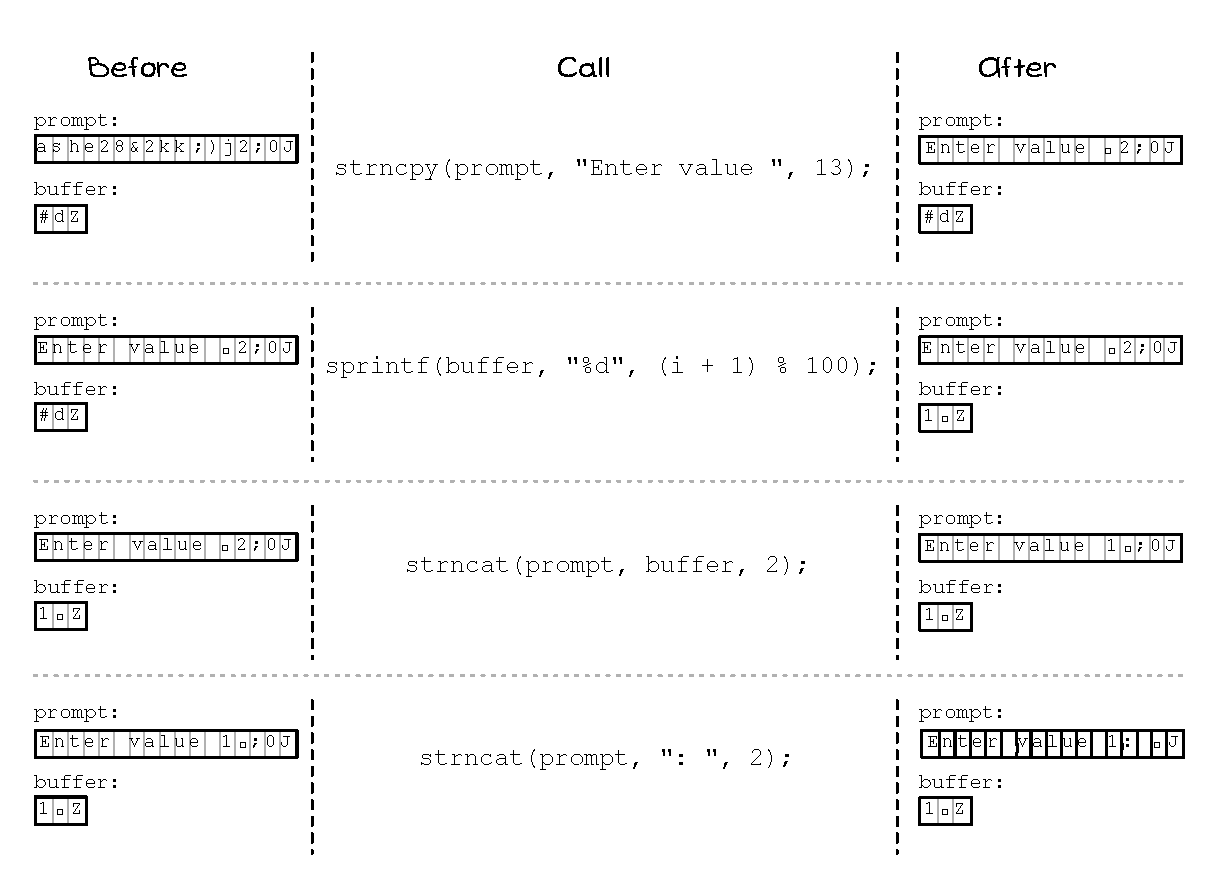
\includegraphics[width=\textwidth]{./topics/arrays/images/CStringOps} 
   \caption{Example usage of c-string functions from the Statistics Calculator}
   \label{fig:cstringops}
\end{figure}

\mynote{
\begin{itemize}
  \item The steps shown in \fref{fig:cstringops} perform the following actions:
  \begin{enumerate}
      \item The first instruction uses \texttt{strncpy} to copy the characters in `\texttt{Enter value}' into the \texttt{prompt}. The \texttt{null} character must also be copied so that \texttt{strncat} knows where the string currently ends.
      \item Step 2 uses \texttt{sprintf} to print the decimal value of \texttt{(i + 1) \% 100} into the \texttt{buffer}. This uses \texttt{\% 100} so that only two characters\footnote{\texttt{(i + 1) \% 100} is the remainder of the value i incremented by one after dividing by 100. This ensures that it is always between 0 and 99. For example, when \texttt{i} is 106, \texttt{i + 1} is 107, and \texttt{107 \% 100} is 7, the remainder of dividing 107 by 100.} and the terminal are ever written into the \texttt{buffer}. 
      This assumes that the value of \texttt{i} is 0, so \texttt{i + 1} is \texttt{1}.
      \item Next \texttt{strncat} is used to concatenate \texttt{prompt} and \texttt{buffer}. This copies the text in \texttt{buffer} to the end of \texttt{prompt}, and makes sure that there is a \texttt{null} character at the end. So the \texttt{n} in this case indicate the maximum number of actual characters to add to the destination, as the \texttt{null} is effectively moved in this function.
      \item The operation is completed by concatenating the final `\texttt{: }' to the end of the string.
  \end{enumerate}
  \item Notice that there is one additional character left in this \texttt{prompt} at the end, this gives space for two digit values, e.g. `\texttt{Enter value 10:}'.
\end{itemize}
}


% subsubsection example_use_of_c_string_functions (end)

% subsection c_string (end)

% section more_data_types_in_c (end)

% ========================
% = Understanding Arrays =
% ========================

\clearpage
\def\pageLang{none}
\section{Understanding Arrays} % (fold)
\label{sec:understanding_arrays}

\nameref{sub:array}s offer a means of storing and working with a list of values in your code. Each array has a number of elements, each of which has a value, and can be accessed using an index. Together with the \nameref{sub:for_loop}, arrays provide a means of managing multiple values in your code. The following illustrations show how these work in the computer, and should help you better understand how arrays can be used within your code.

\subsection{Understanding Populate Array} % (fold)
\label{sub:understanding_populate_array}

\sref{sub:designing_statistics_calculator} \nameref{sub:designing_statistics_calculator} outlined the pseudocode and flowcharts for a small statistics programs. This included a number of functions and procedures that helped divide the Program's code into smaller units of work. One of these procedures was \texttt{Populate Array}, discussed in \sref{ssub:populating_the_array} \nameref{ssub:populating_the_array}. This procedure is responsible for reading values from the user and using these to populate the program's array, and the flowchart for this logic is shown in \fref{fig:populate-array-flow-understanding}.

\begin{figure}[htbp]
   \centering
   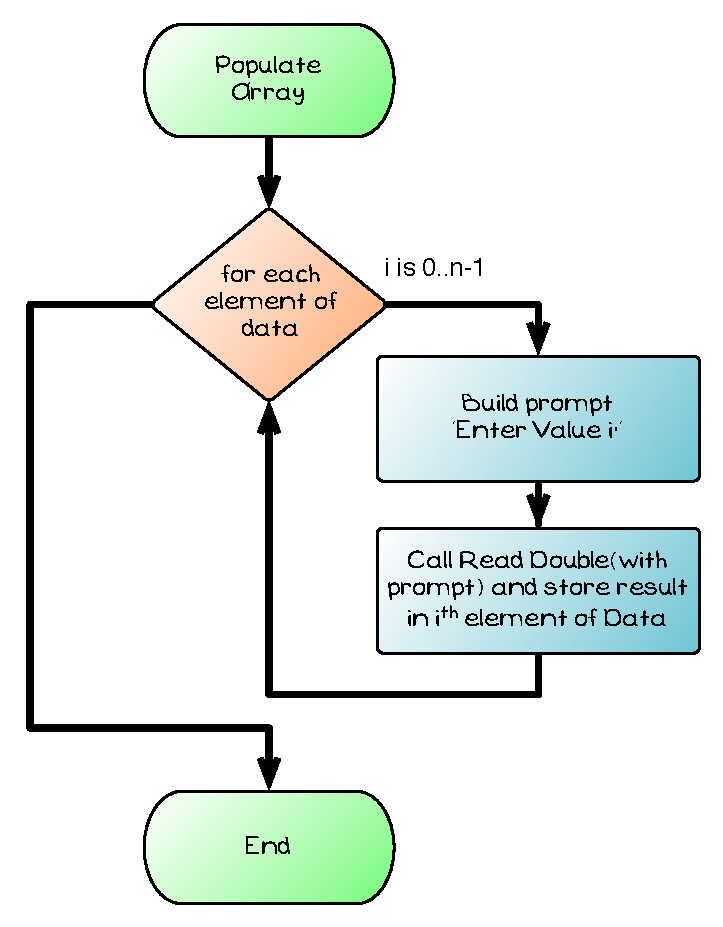
\includegraphics[width=0.5\textwidth]{./topics/arrays/diagrams/PopulateArray} 
   \caption{Flowchart showing the process for \texttt{Populate Array}, from \fref{fig:populate-array-flow}}
   \label{fig:populate-array-flow-understanding}
\end{figure}

The following illustrations will show this code running to populate an array that contains three values. This will show how the array is passed by reference, and how the for loop works together with the array to populate all elements.

\clearpage
\subsubsection{Main starts, and the array is allocated space} % (fold)
\label{ssub:main_starts_and_the_array_is_allocated_space}

All local variables are allocated space on the Stack when the function or procedure they are declared in is called. In this example the \texttt{Main} procedure is executed and space is allocated for its \texttt{my\_data} variable. This variable is an \nameref{sub:array} that is used to store three \texttt{double} values. When \texttt{Main} is loaded onto the Stack there is space allocated for three \texttt{double} values associated with the \texttt{my\_data} variable.

\begin{figure}[htbp]
   \centering
   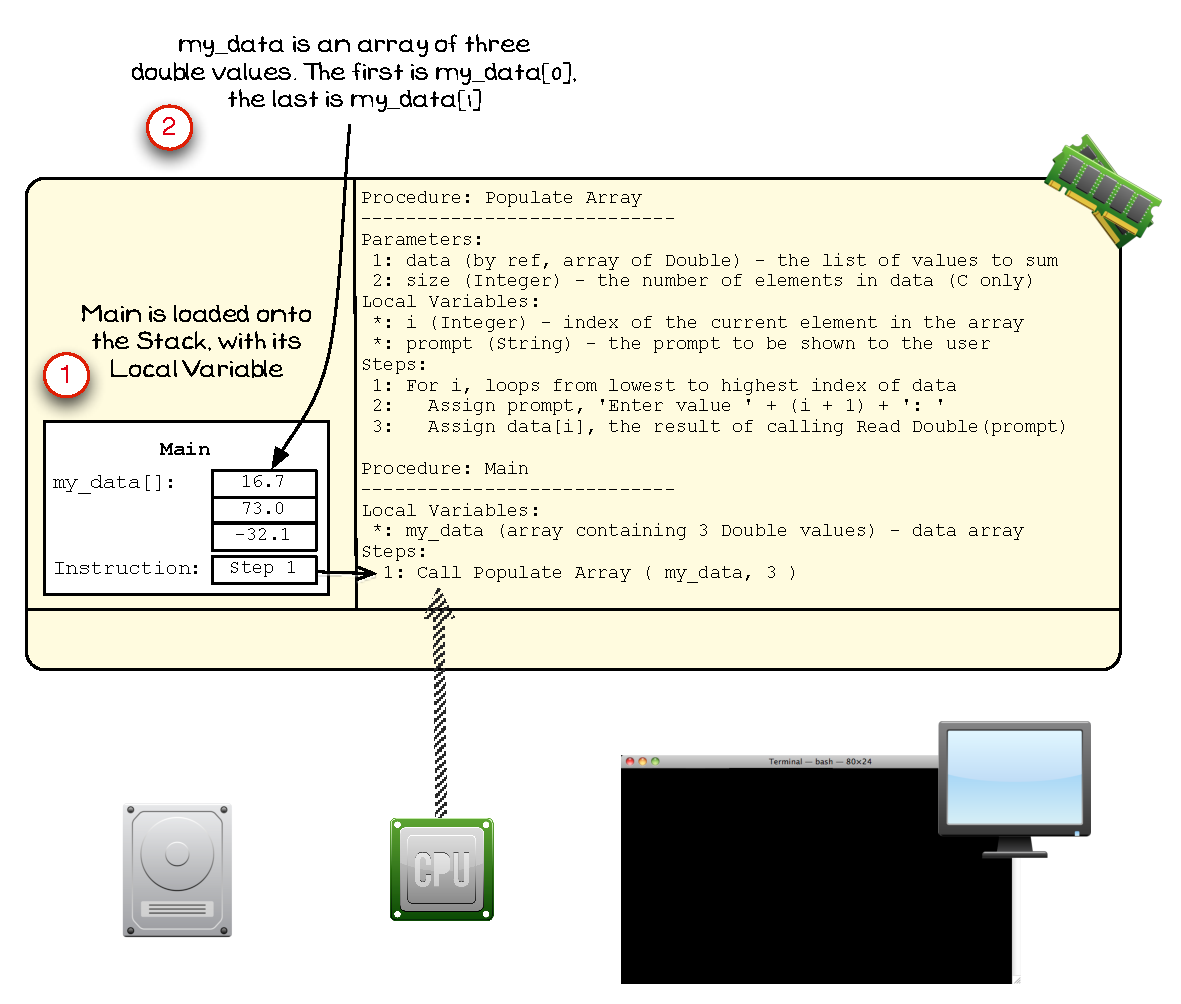
\includegraphics[width=\textwidth]{./topics/arrays/images/PopulateArray1} 
   \caption{When the program starts \texttt{Main} allocates space for its local variables, including the array}
   \label{fig:populate-array-vis-1}
\end{figure}

\mynote{
\begin{itemize}
  \item In \fref{fig:populate-array-vis-1} the indicated areas show the following:
  \begin{enumerate}
    \item The Program starts and \texttt{Main} is loaded onto the stack, allocating space for its local variables.
    \item The \texttt{my\_data} array is allocated space to store its values.
  \end{enumerate}
  \medskip
  \item Notice that the three values in the array are allocated next to each other.
  \item The indexes can be used to access the array's elements. The index value determines the number of elements that must be skipped to find where the value is stored.
\end{itemize}
}
% subsubsection main_starts_and_the_array_is_allocated_space (end)

\clearpage
\subsubsection{Populate array is called, and a reference to \texttt{my{\textunderscore}data} passed in} % (fold)
\label{ssub:populate_array_is_called_and_a_reference_to_my_data_passed_in}

\texttt{Populate Array} is called as the first step in \texttt{Main}. This is passed the \texttt{my\_data} variable (pass by reference), rather than being passed the values from within that variable. This gives the \texttt{data} parameter access to the memory where \texttt{my\_data} is stored.

\begin{figure}[htbp]
   \centering
   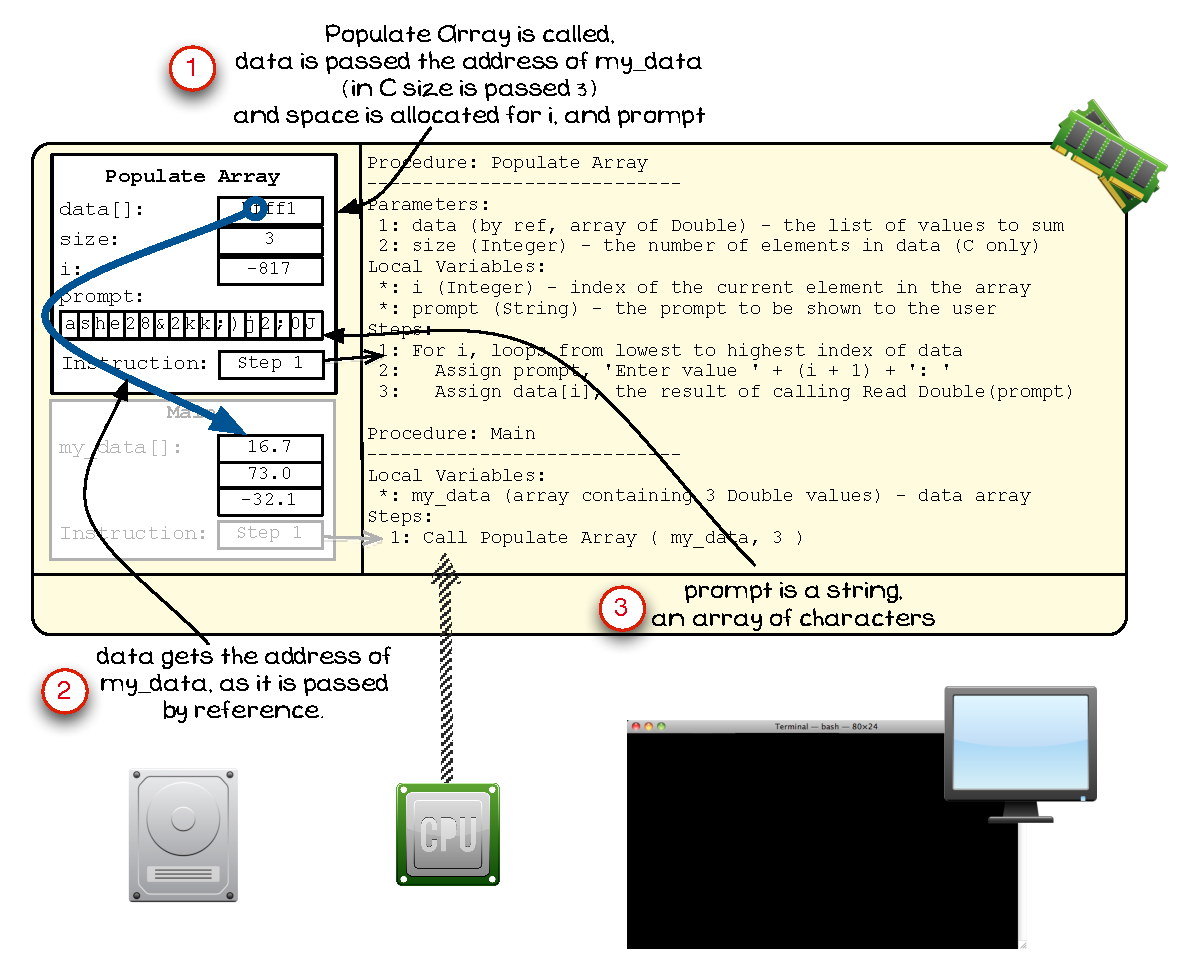
\includegraphics[width=\textwidth]{./topics/arrays/images/PopulateArray2} 
   \caption{Populate array is called, and a reference to the \texttt{my\_data} array is pass to its \texttt{data} parameter}
   \label{fig:populate-array-vis-2}
\end{figure}

\mynote{
\begin{itemize}
  \item In \fref{fig:populate-array-vis-2} the indicated areas show the following:
  \begin{enumerate}
    \item When \texttt{Populate Array} is called it is loaded onto the Stack. Its \texttt{data} parameter receives the address of \texttt{my\_data} from \texttt{Main}. In C the value 3 would also be passed to the \texttt{size} parameter, as C does not keep track of the length of the array for you. At the same time space for \texttt{Populate Array}'s local variables \texttt{i} and \texttt{prompt} are allocated on the Stack.
    \item Notice that in \texttt{Populate Array} the \texttt{data} parameter only stores the address of the array, as it is passed by reference. This saves time and space, and is needed in this case as the procedure wants to store data into the variable passed to this parameter.
    \item The \texttt{prompt} local variable is also an array. It is allocated spaces on the stack as is done for all local variables. 
  \end{enumerate}
  \medskip
  \item Arrays are allocated a contiguous area of memory to store its elements.
  \item A String is an array of characters.
\end{itemize}
}

% subsubsection populate_array_is_called_and_a_reference_to_my\_data_passed_in (end)

\clearpage
\subsubsection{Step 1 of \texttt{Populate Array} is run} % (fold)
\label{ssub:step_1_of_populate_array_is_run}

Step 1 of \texttt{Populate Array} initialises the for loop's control variable (\texttt{i} in this case). This variable keeps track of the times the loop body has executed, and can be used to get the \emph{current} value from the array.

\begin{figure}[htbp]
   \centering
   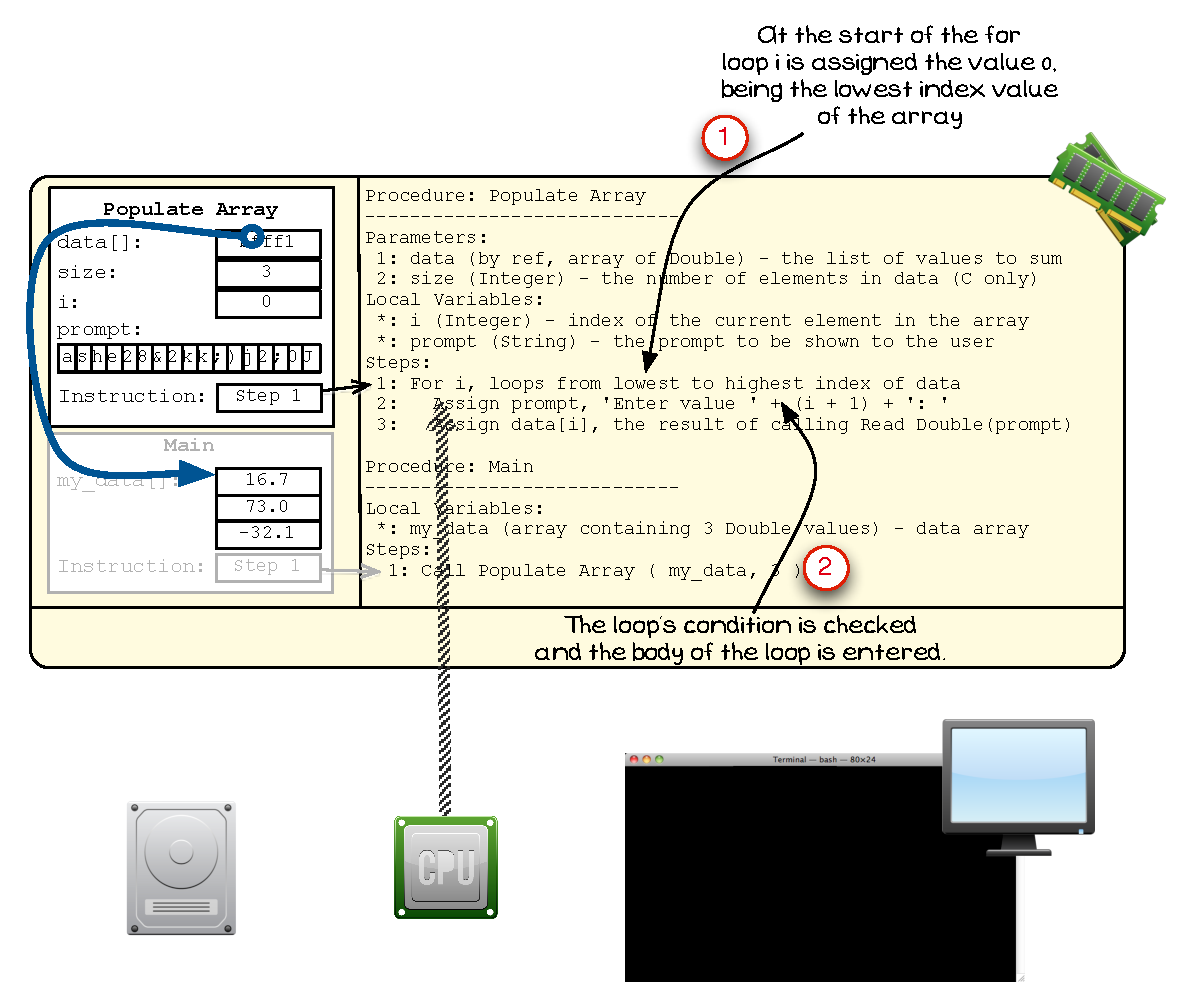
\includegraphics[width=\textwidth]{./topics/arrays/images/PopulateArray3} 
   \caption{Step 1 of \texttt{Populate Array} is called, and the for loop sets i to the lowest index of the \texttt{data} array}
   \label{fig:populate-array-vis-3}
\end{figure}

\mynote{
\begin{itemize}
  \item In \fref{fig:populate-array-vis-3} the indicated areas show the following:
  \begin{enumerate}
    \item Step 1 of \texttt{Populate Array} is a for loop. The first action of the for loop is to initialise the value of \texttt{i} to the \emph{lowest index value} of the \texttt{data} array. The lowest index is 0, so \texttt{i} is assigned the value 0.
    \item Next the loop checks its condition, it is loop from 0 to 2, and has not passed 2 so the body of the loop will be executed. This will be checked again when the for loop ends.
  \end{enumerate}
  \medskip
  \item The first action of a for loop is to initialise the value of the control variable.
  \item When processing each element of an array the for loop should initialise the control variable to 0, the first index of the array.
\end{itemize}
}

% subsubsection step_1_of_populate_array_is_run (end)

\clearpage
\subsubsection{Step 2 constructs the prompt to be shown to the user} % (fold)
\label{ssub:step_2_constructs_the_prompt_to_be_shown_to_the_user}

The user needs to be told what to enter. The \texttt{prompt} is a string that will contain this message so that it can be passed to \texttt{Read Double}. The value for the prompt will use the loop's control variable (the counter) so that the user known which value they are up to.

\begin{figure}[htbp]
   \centering
   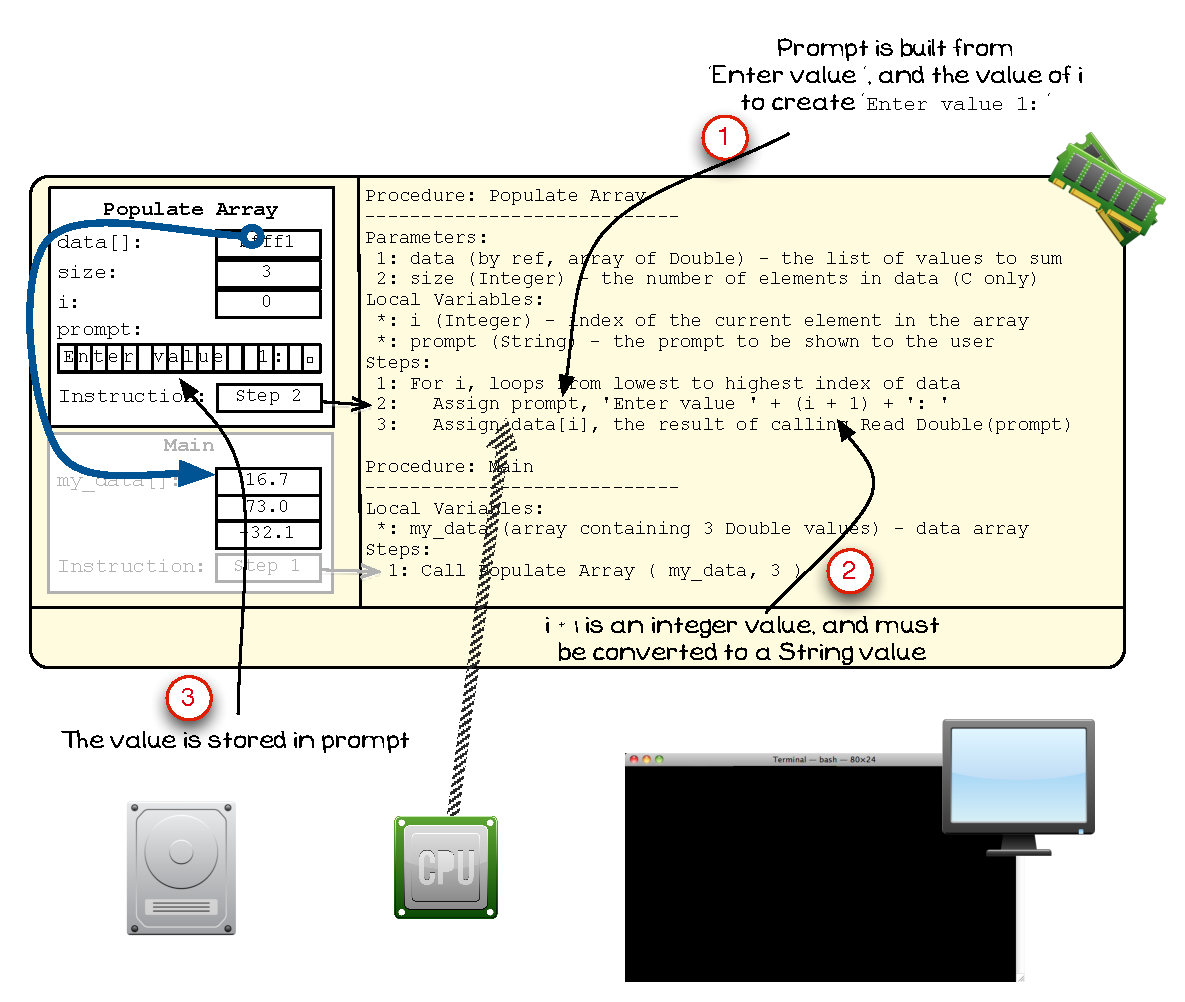
\includegraphics[width=\textwidth]{./topics/arrays/images/PopulateArray4} 
   \caption{Step 2 builds the prompt \texttt{Enter value 1: } which will be shown to the user}
   \label{fig:populate-array-vis-4}
\end{figure}

\mynote{
\begin{itemize}
  \item In \fref{fig:populate-array-vis-4} the indicated areas show the following:
  \begin{enumerate}
    \item Step 2 of \texttt{Populate Array} builds the prompt by concatenating `\texttt{Enter Value}' with \texttt{i + 1} and `\texttt{: }'.
    \item To achieve this \texttt{i + 1} must be converted from an Integer to a String.
    \item The result is stored in the \texttt{prompt} variable.
  \end{enumerate}
  \medskip
  \item This action will be performed each time the loop executes. In this case the value stored in \texttt{prompt} will be `\texttt{Enter value  1: }'.
  \item The small square shown at the end of the \texttt{prompt} represents the overhead. In C this is the \emph{sentinel} value, in Pascal it is the length\footnote{Pascal actually stores the length at the start of the string, but the idea is the same.} of the array.
\end{itemize}
}


% subsubsection step_2_constructs_the_prompt_to_be_shown_to_the_user (end)

\clearpage
\subsubsection{Step 3 reads a value from the user and stores it in the array at index 0} % (fold)
\label{ssub:step_3_reads_a_value_from_the_user_and_stores_it_in_the_array_at_index_0}

The next step calls the \texttt{Read Double} function. This is responsible for reading a value from the user, and returning it to the caller. The value returned is then stored in an element of the array. The \texttt{i} variable is read to determine the position where this value should be stored. This means that you can think of \texttt{i} as referring to the \emph{current} element of the array.

\begin{figure}[htbp]
   \centering
   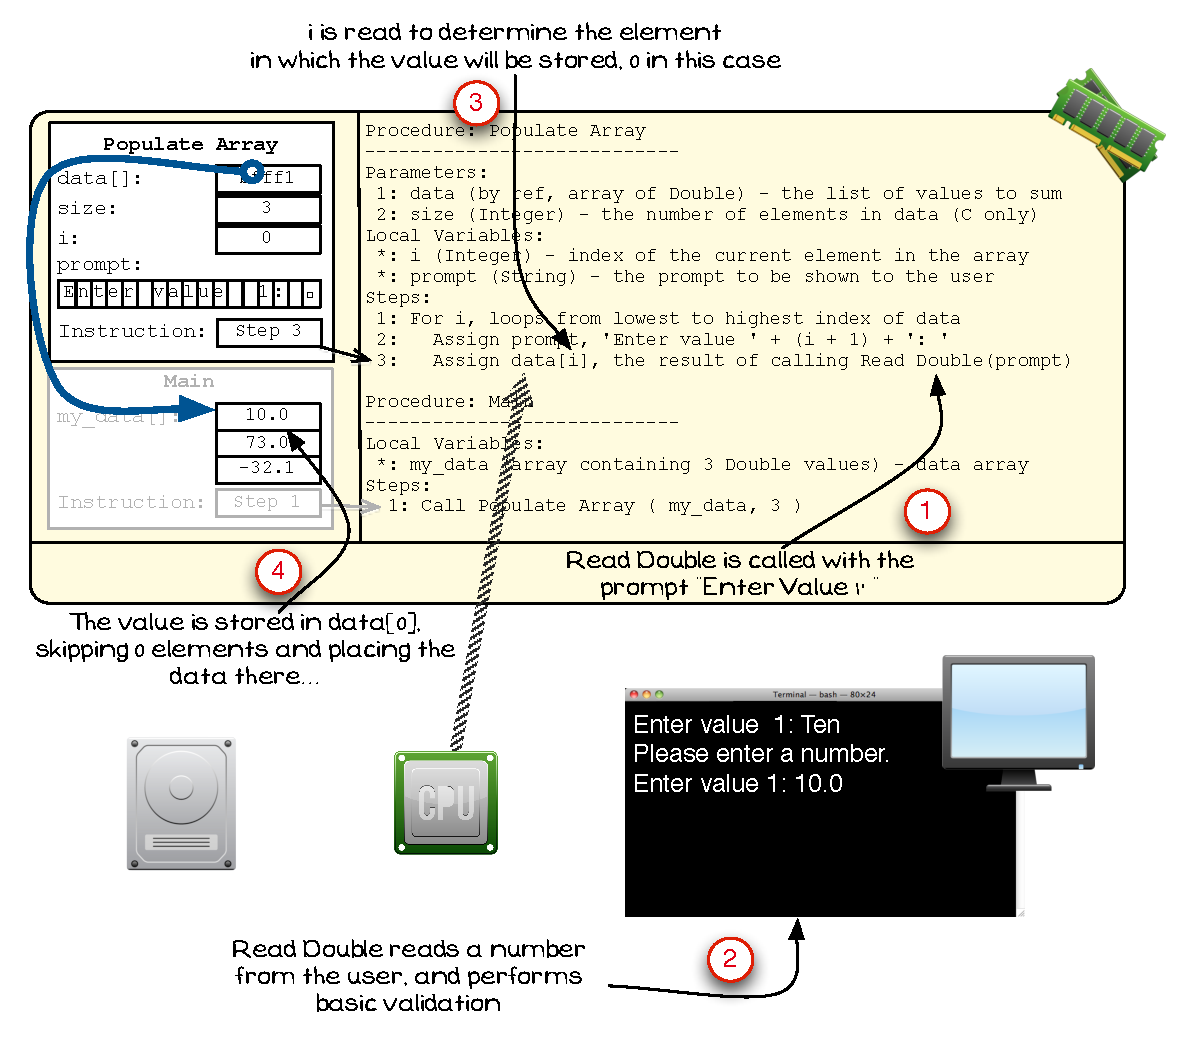
\includegraphics[width=\textwidth]{./topics/arrays/images/PopulateArray5} 
   \caption{Step 3 reads a \texttt{double} value from the user and stores it in \texttt{data[i]}}
   \label{fig:populate-array-vis-5}
\end{figure}

\mynote{
\begin{itemize}
  \item In \fref{fig:populate-array-vis-5} the indicated areas show the following:
  \begin{enumerate}
    \item Step 3 of \texttt{Populate Array} calls \texttt{Read Double}, passing across the prompt to be shown to the user.
    \item Within \texttt{Read Double} the value is read from the Terminal. This includes some validation to make sure that the value entered is a number.
    \item To determine where the value is stored the computer needs to evaluate the expression used to index the array. In this case that is the value of the \texttt{i} variable.
    \item The \texttt{data} reference is followed, and \texttt{0} elements skipped, to find the location where the data should be stored. 
  \end{enumerate}
  \medskip
  \item Notice that this has stored the value in \texttt{my\_data}, as \texttt{data} is passed by reference.
\end{itemize}
}

% subsubsection step_3_reads_a_value_from_the_user_and_stores_it_in_the_array_at_index_0 (end)

\clearpage
\subsubsection{Control returns to Step 1 as the loop body has ended} % (fold)
\label{ssub:control_returns_to_step_1_as_the_loop_body_has_ended}

At the end of the loop body the for loop performs two actions. It has finished the first pass through the loop, so its control variable (the counter) needs to be incremented to 1. Then it needs to jump back to check its condition. This will determine if the loop's body is executed again or skipped. In this case \texttt{i} is still in the defined range so the loop's body is run again.

\begin{figure}[htbp]
   \centering
   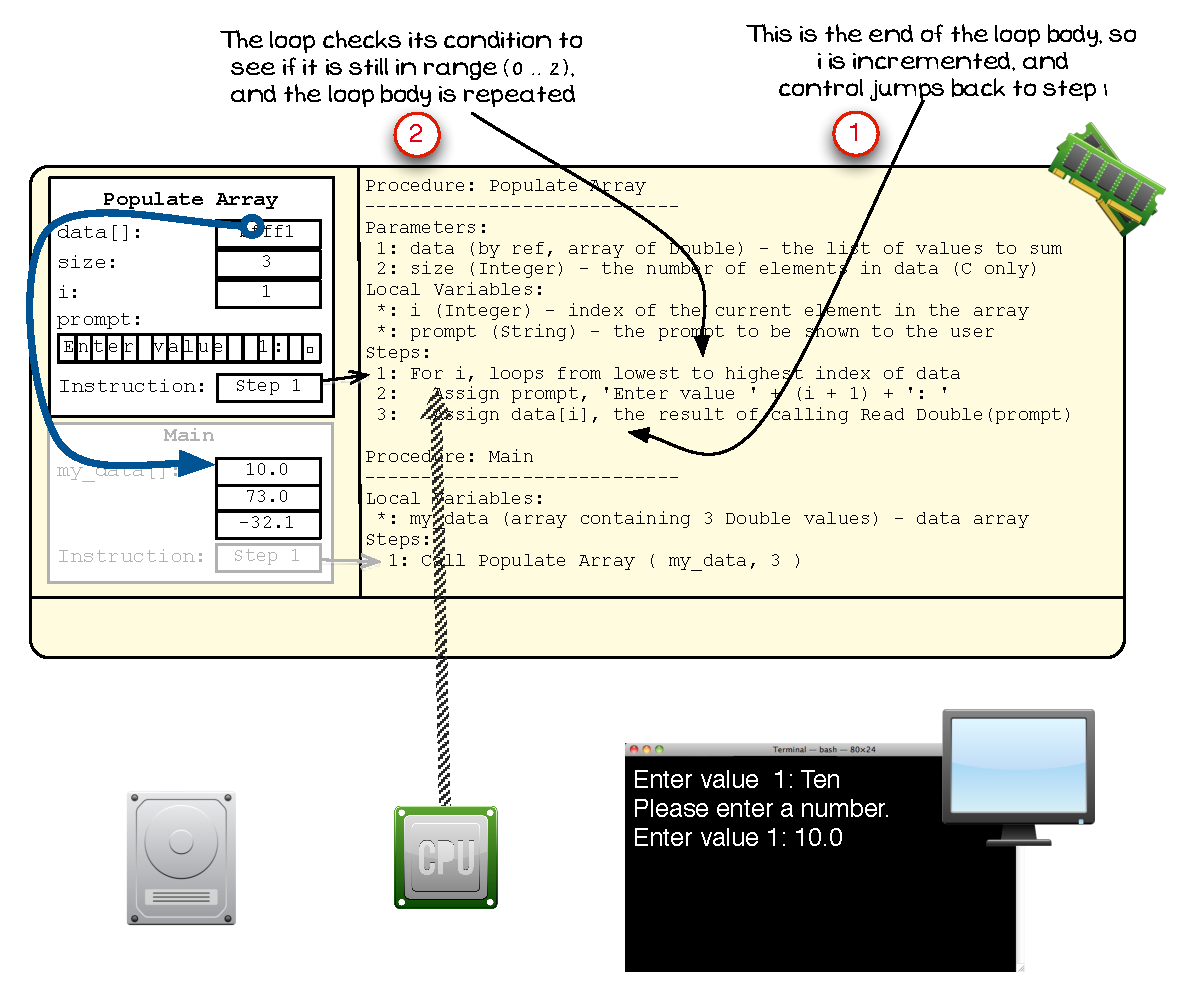
\includegraphics[width=\textwidth]{./topics/arrays/images/PopulateArray6} 
   \caption{At the end of the loop body \emph{i} is incremented and control jumps back to check the loop's condition}
   \label{fig:populate-array-vis-6}
\end{figure}

\mynote{
\begin{itemize}
  \item In \fref{fig:populate-array-vis-6} the indicated areas show the following:
  \begin{enumerate}
    \item The end of the loop body indicates that two things needs to occur. Firstly the value of \texttt{i} needs to be incremented, and then control needs to jump back to check the condition of the loop (step 1).
    \item The loop's condition checks if \texttt{i} is still in range (\texttt{i} is in the range \texttt{0..2}, coded as \texttt{i < size} in C). As it is still in range the loop's body will execute again.
  \end{enumerate}
  \medskip
\end{itemize}
}

% subsubsection control_returns_to_step_1_as_the_loop_body_has_ended (end)

\clearpage
\subsubsection{Second prompt is built asking the user to enter value 2} % (fold)
\label{ssub:second_prompt_is_built_asking_the_user_to_enter_value_2}

Back at step 2 again, the prompt needs to be recreated. This time its message will be `\texttt{Enter value 2: }'. The process to create this is the same, with the value of \texttt{i + 1} being converted to a String, and the three parts concatenated together and stored in \texttt{prompt}. This overrides the details in the existing array, reusing the same memory to store these values.

\begin{figure}[htbp]
   \centering
   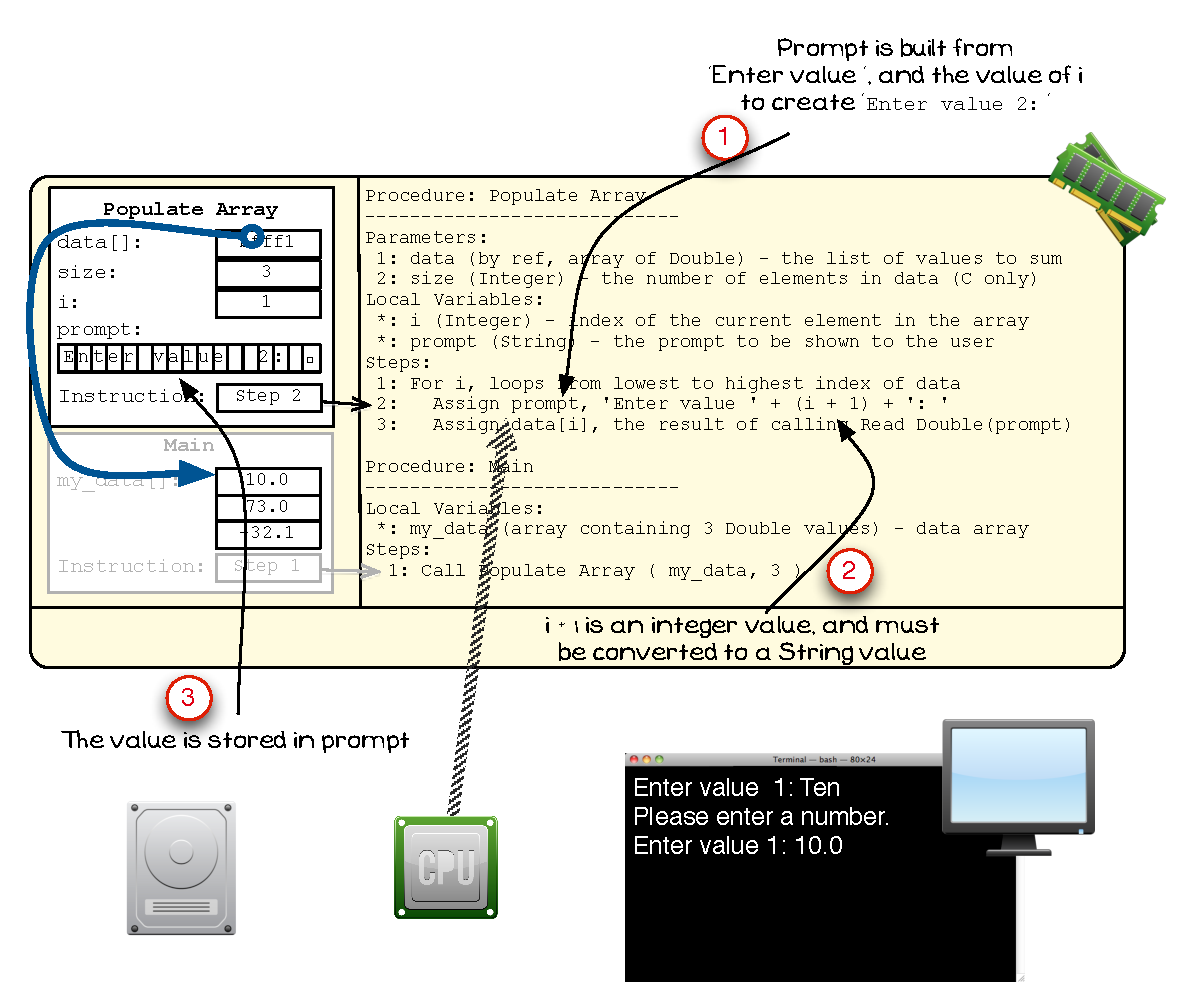
\includegraphics[width=\textwidth]{./topics/arrays/images/PopulateArray7} 
   \caption{Step 2 builds the prompt \texttt{Enter value 2: } which will be shown to the user}
   \label{fig:populate-array-vis-7}
\end{figure}

\mynote{
\begin{itemize}
  \item In \fref{fig:populate-array-vis-7} the indicated areas show the following:
  \begin{enumerate}
    \item Step 2 of \texttt{Populate Array} builds the prompt by concatenating `\texttt{Enter Value}' with \texttt{i + 1} and `\texttt{: }'.
    \item To achieve this \texttt{i + 1} must be converted from an Integer to a String.
    \item The result is stored in the \texttt{prompt} variable.
  \end{enumerate}
  \medskip
  \item Notice that this is using the same location to store its data.
  \item The small square shown at the end of the \texttt{prompt} represents the overhead. In C this is the \emph{sentinel} value, in Pascal it is the length\footnote{Pascal actually stores the length at the start of the string, but the idea is the same.} of the array.
\end{itemize}
}

% subsubsection second_prompt_is_built_asking_the_user_to_enter_value_2 (end)

\clearpage
\subsubsection{\texttt{Populate Array} stores the second value read into \texttt{data[1]}} % (fold)
\label{ssub:populate_array_stores_the_second_value_read_into_data[1]}

Step 3 uses \texttt{Read Double} again to get the value to store in the second element of the array. To find where this should be stored the computer calculates the value of the index, reading this from the \texttt{i} variable. The value returned from \texttt{Read Double} is then stored in the array referred to by \texttt{data}, at index \texttt{1}.

\begin{figure}[htbp]
   \centering
   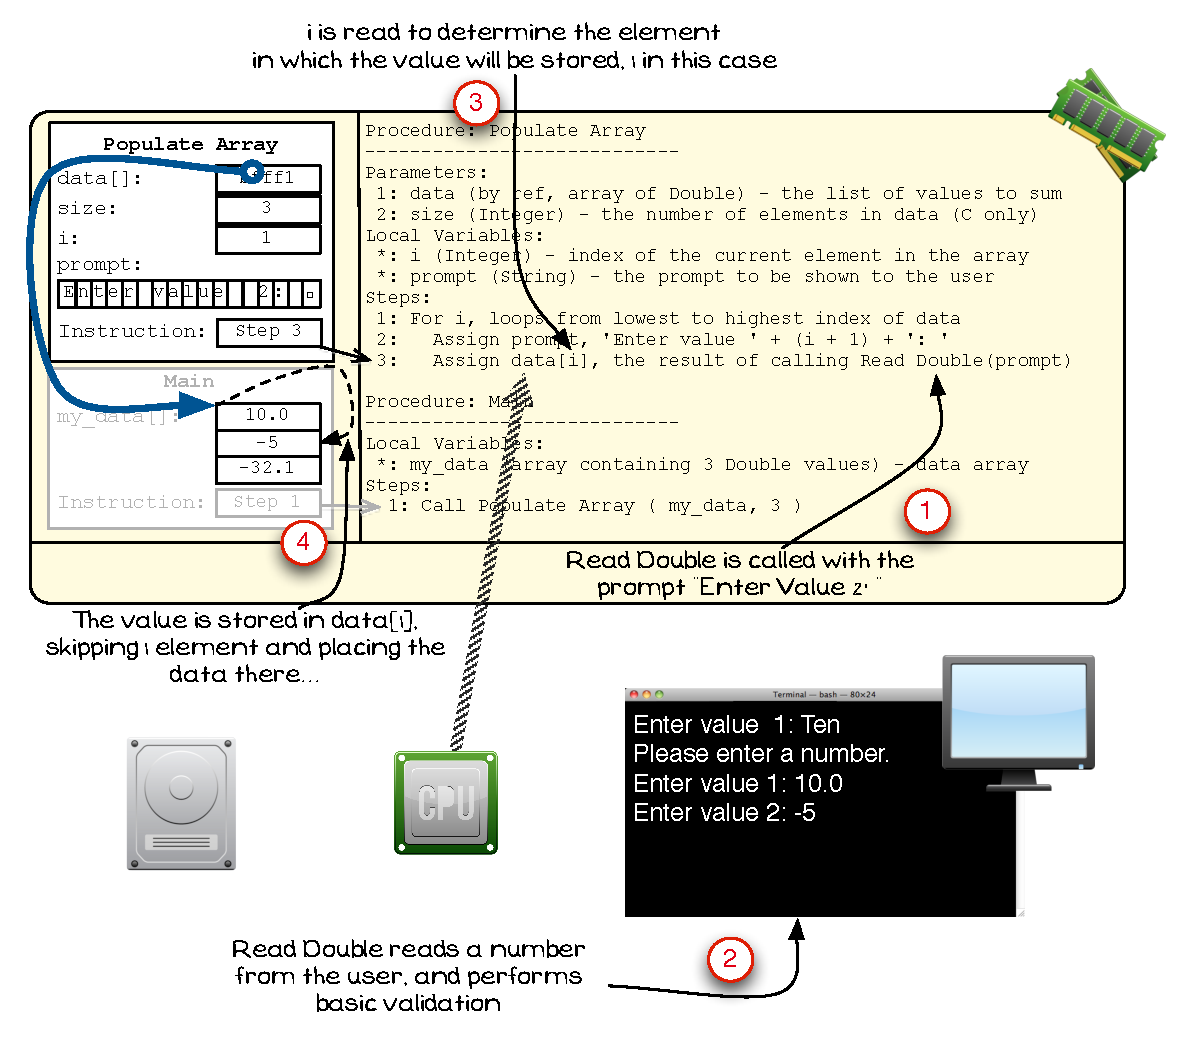
\includegraphics[width=\textwidth]{./topics/arrays/images/PopulateArray8} 
   \caption{The second value read is stored in \texttt{data[1]}}
   \label{fig:populate-array-vis-8}
\end{figure}

\mynote{
\begin{itemize}
  \item In \fref{fig:populate-array-vis-8} the indicated areas show the following:
  \begin{enumerate}
    \item Step 3 of \texttt{Populate Array} calls \texttt{Read Double}, passing across the prompt to be shown to the user.
    \item Within \texttt{Read Double} the value is read from the Terminal. This includes some validation to make sure that the value entered is a number.
    \item The value of the index is now \texttt{1}, as read from variable \texttt{i}.
    \item The \texttt{data} reference is followed, and \texttt{1} element is skipped, to find the location where the data should be stored.
  \end{enumerate}
  \medskip
\end{itemize}
}

% subsubsection populate_array_stores_the_second_value_read_into_data[1] (end)

\clearpage
\subsubsection{\texttt{i} is incremented again, and control returns to Step 1 to determine if loop runs again} % (fold)
\label{ssub:i_is_incremented_again_and_control_returns_to_step_1_to_determine_if_loop_runs_again}

The end of the for loop's body has been reached again, so it performs two actions: it increments its control variable (\texttt{i} in this case) and jumps back to check its condition (step 1). The condition then determines if the loop's body is to be executed again or skipped. In this case \texttt{i} is still in the defined range so the loop's body is run a third time.

\begin{figure}[htbp]
   \centering
   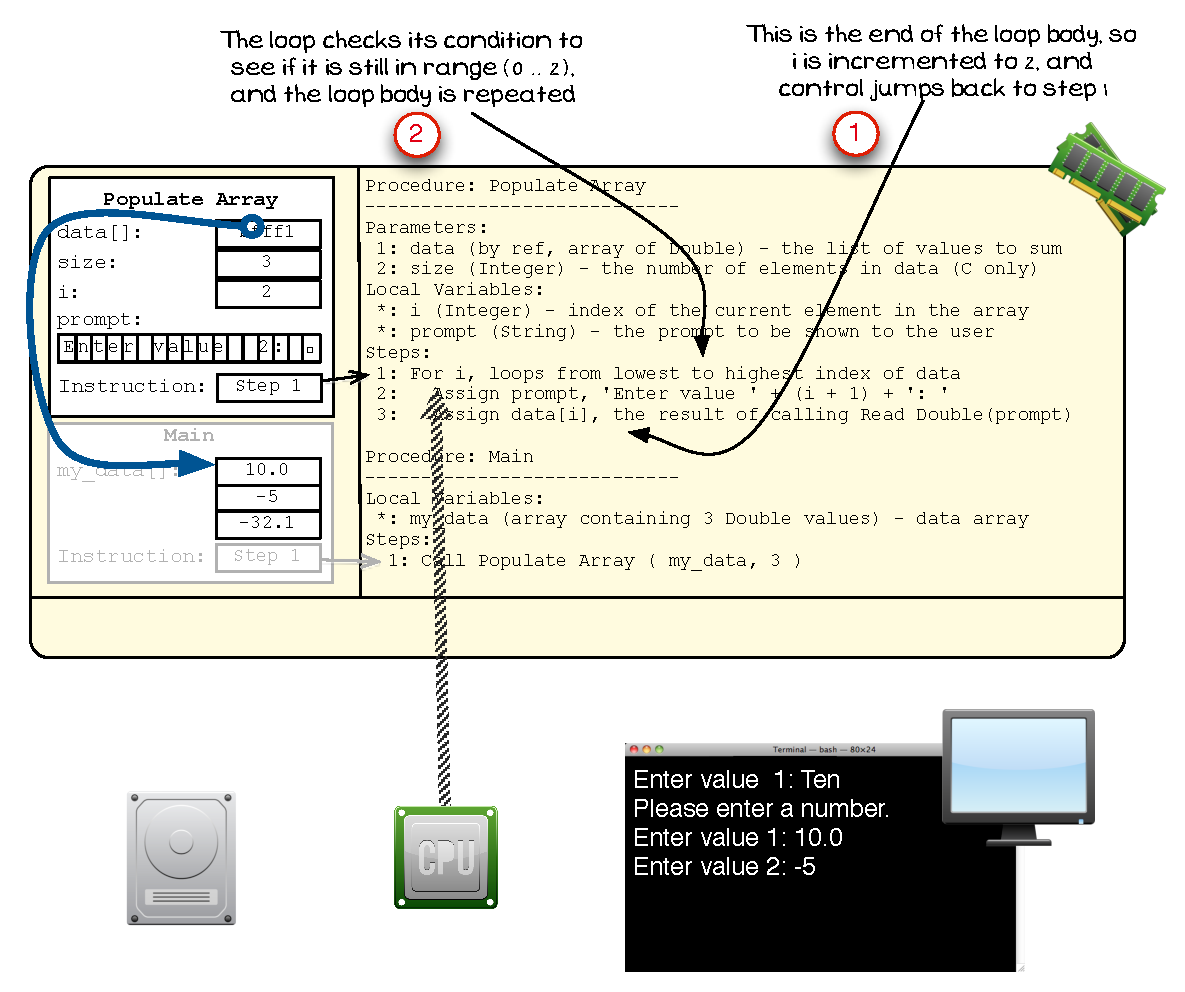
\includegraphics[width=0.98\textwidth]{./topics/arrays/images/PopulateArray9} 
   \caption{At the end of the loop body \emph{i} is incremented and control jumps back to check the loop's condition}
   \label{fig:populate-array-vis-9}
\end{figure}

\mynote{
\begin{itemize}
  \item In \fref{fig:populate-array-vis-9} the indicated areas show the following:
  \begin{enumerate}
    \item The end of the loop body indicates that two things needs to occur: the value of \texttt{i} is incremented, and control jump back to check the condition of the loop.
    \item The loop's condition checks if \texttt{i} is still in range (\texttt{i} is in the range \texttt{0..2}, coded as \texttt{i < size} in C). As it is still in range the loop's body is execute again.
  \end{enumerate}
  \medskip
  \item These same actions always occur at the end of the for loop. It increments its control variable, and jumps back to check its condition.
\end{itemize}
}

\csection{The C for loop can be used for more than just counting. At the end of the loop the instructions from the \nameref{sub:c_for_loop}'s \emph{increment} occur, typically something like \texttt{i++}.}


% subsubsection i_is_incremented_again_and_control_returns_to_step_1_to_determine_if_loop_runs_again (end)

\clearpage
\subsubsection{Third prompt is built asking the user to enter value 3} % (fold)
\label{ssub:third_prompt_is_built_asking_the_user_to_enter_value_3}

Back at step 2 for the third time. This step recreates the prompt, this time with the message `\texttt{Enter value 3: }'. The process to create this is the same as before, with the value of \texttt{i + 1} being converted to a String, and the three parts concatenated together and stored in \texttt{prompt}. Remember that this overrides the data currently in the \texttt{prompt} array.

\begin{figure}[htbp]
   \centering
   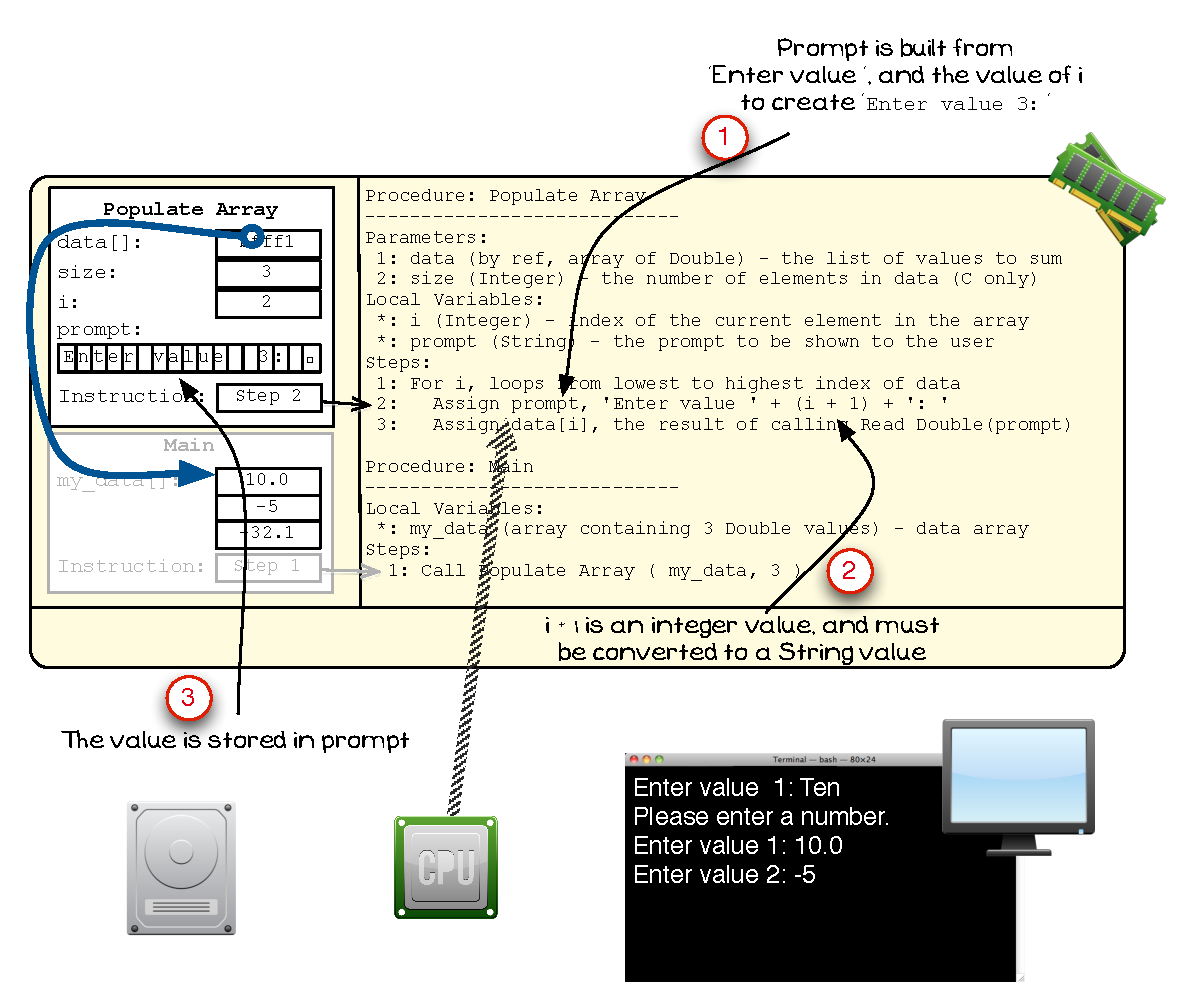
\includegraphics[width=\textwidth]{./topics/arrays/images/PopulateArray10} 
   \caption{Step 2 builds the prompt \texttt{Enter value 3: } which will be shown to the user}
   \label{fig:populate-array-vis-10}
\end{figure}

\mynote{
\begin{itemize}
  \item In \fref{fig:populate-array-vis-10} the indicated areas show the following:
  \begin{enumerate}
    \item Step 2 of \texttt{Populate Array} builds the prompt by concatenating `\texttt{Enter Value}' with \texttt{i + 1} and `\texttt{: }'.
    \item To achieve this \texttt{i + 1} must be converted from an Integer to a String.
    \item The result is stored in the \texttt{prompt} variable.
  \end{enumerate}
  \medskip
\end{itemize}
}

% subsubsection third_prompt_is_built_asking_the_user_to_enter_value_3 (end)

\clearpage
\subsubsection{\texttt{Populate Array} stores the third value read into \texttt{data[2]}} % (fold)
\label{ssub:populate_array_stores_the_third_value_read_into_data[2]}

Once again, step 3 uses \texttt{Read Double} get the value to store in the array. In this case \texttt{i} indicates that this should be stored in the element at index 2 (skipping 2 elements, so storing the value in the third).

\begin{figure}[htbp]
   \centering
   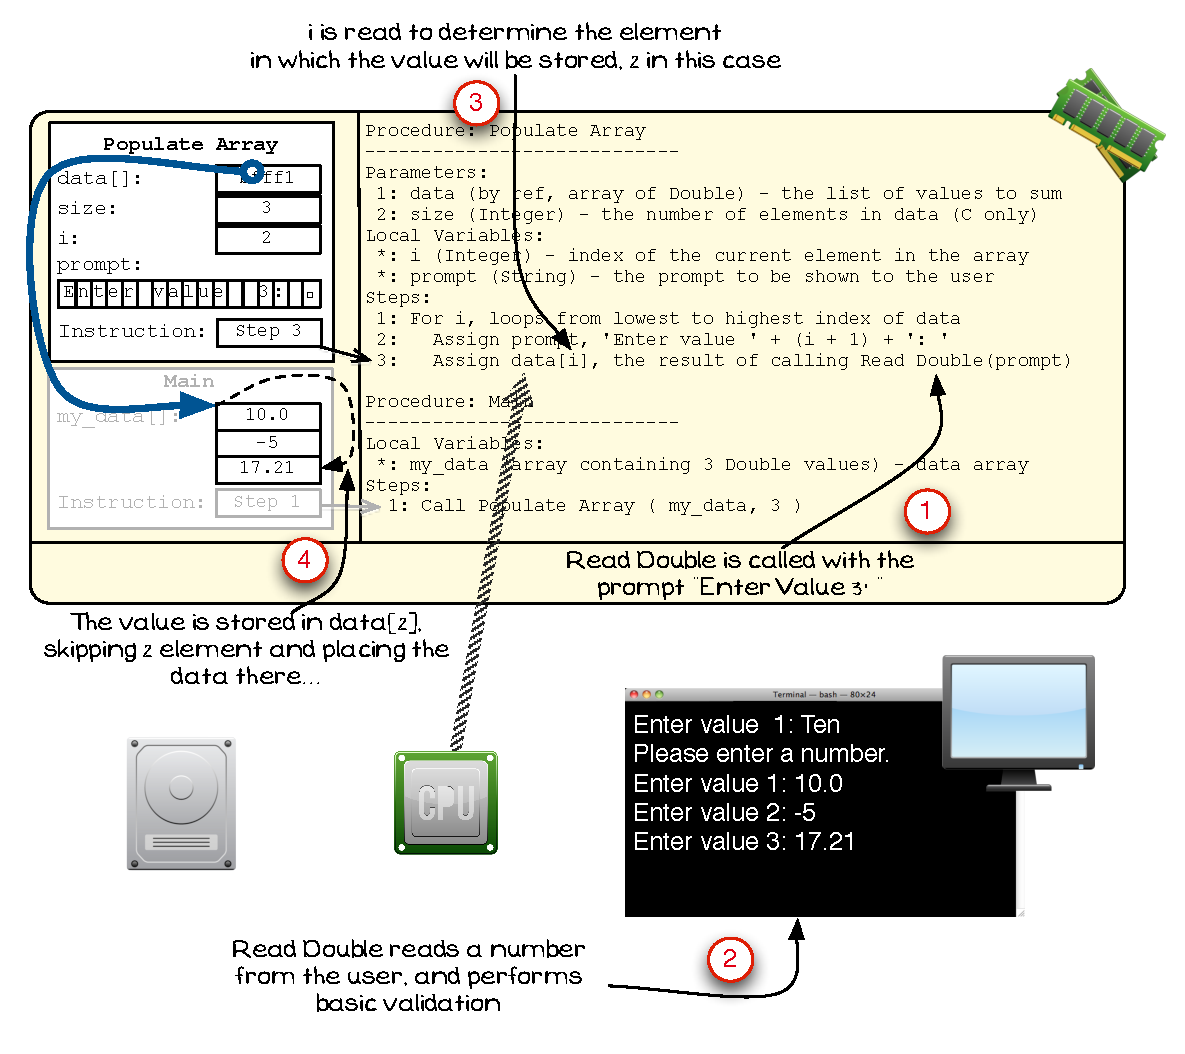
\includegraphics[width=\textwidth]{./topics/arrays/images/PopulateArray11} 
   \caption{The second value read is stored in \texttt{data[1]}}
   \label{fig:populate-array-vis-11}
\end{figure}

\mynote{
\begin{itemize}
  \item In \fref{fig:populate-array-vis-11} the indicated areas show the following:
  \begin{enumerate}
    \item Step 3 of \texttt{Populate Array} calls \texttt{Read Double} again.
    \item Within \texttt{Read Double} the value is read from the Terminal.
    \item The value of the index is now \texttt{2}, as read from variable \texttt{i}.
    \item The \texttt{data} reference is followed, and \texttt{2} elements are skipped to find the location where the data should be stored.
  \end{enumerate}
  \medskip
  \item Notice how over these three loops \texttt{i} has been used to determine which element is the \emph{current element}. The loop's processing is the same, but changing \texttt{i} means that this action is applied to each element in the array one at a time.
  \item The loop's body determines the action to apply to the \texttt{$i^{th}$} element of the array.
  \item The for loop then updates \texttt{i} so that the body is applied to \emph{each} element of the array.
\end{itemize}
}

% subsubsection populate_array_stores_the_third_value_read_into_data[2] (end)

\clearpage
\subsubsection{\texttt{i} is incremented again, and control jumps back to check the condition a fourth time} % (fold)
\label{ssub:i_is_incremented_again_and_control_jumps_back_to_check_the_condition_a_fourth_time}

The end of the for loop's body has been reached again, so it performs two actions: it increments its control variable (\texttt{i} in this case) and jumps back to check its condition (step 1). This time the value of \texttt{i} is outside the range of the indexes for \texttt{data} (\texttt{0..2}, it is no longer less than 3). This means that the loop's body should not be run again, and control will jump past the body to the next step. As there are no more steps in \texttt{Populate Array} it will end.

\begin{figure}[htbp]
   \centering
   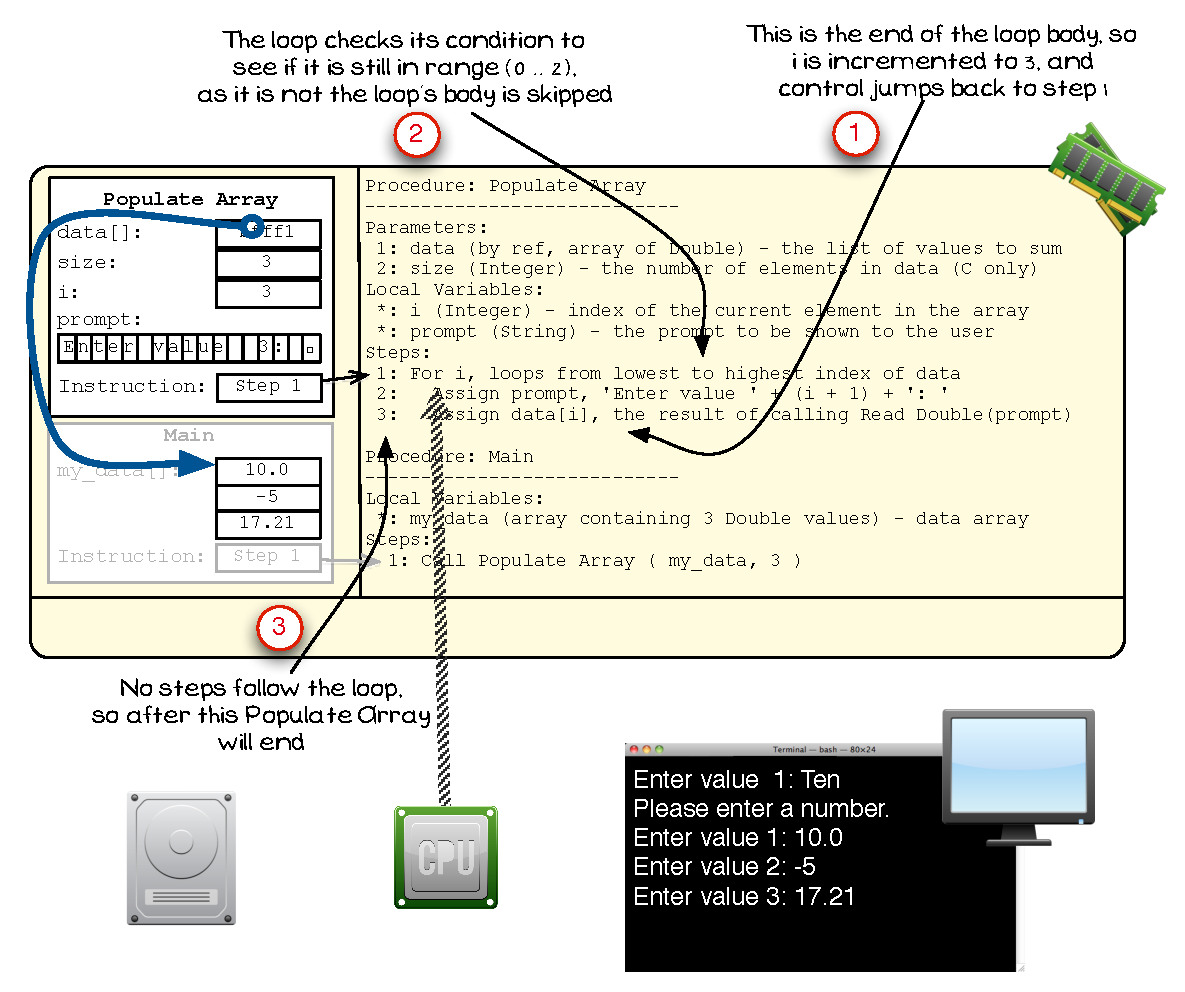
\includegraphics[width=\textwidth]{./topics/arrays/images/PopulateArray12} 
   \caption{At the end of the loop body \emph{i} is incremented and control jumps back to check the loop's condition}
   \label{fig:populate-array-vis-12}
\end{figure}

\mynote{
\begin{itemize}
  \item In \fref{fig:populate-array-vis-12} the indicated areas show the following:
  \begin{enumerate}
    \item The end of the loop body causes the value of \texttt{i} to be incremented, and control jump back to check the condition of the loop.
    \item The loop's condition checks if \texttt{i} is still in range (\texttt{i} is in the range \texttt{0..2}, coded as \texttt{i < size} in C).
    \item \texttt{i} is \textbf{not} in the range \texttt{0..2}, so the loop body is skipped. As there are no more steps in this procedure it ends.
  \end{enumerate}
  \medskip
  \item The condition in the for loop is responsible for determining if the loop runs again. This time the condition indicates that the loop is not to be run again, so control will jump past the end of the loop.
  \item The for loop works like a while loop, with additional logic to keep a counter.
\end{itemize}
}

% subsubsection i_is_incremented_again_and_control_jumps_back_to_check_the_condition_a_fourth_time (end)

\clearpage
\subsubsection{\texttt{Populate Array} ends, and has populated \texttt{Main}'s \texttt{my{\textunderscore}data} array} % (fold)
\label{ssub:populate_array_ends_and_has_populated_main_s_my_data_array}

When \texttt{Populate Array} ends its space on the stack is released so that it can be used again, and control returns to \texttt{Main}. \texttt{Populate Array} was responsible for reading values from the user and storing these in the array passed to it, and if you look at \fref{fig:populate-array-vis-13} you can see that this has been achieved.

The instructions in \texttt{Populate Array} commanded the computer to read a value from the user and store it in the current element (the $i^{th}$ element) of the array. These actions were then repeated by the \nameref{sub:for_loop} \emph{for each} index of the array. Together the for loop and its body allow you to define actions that must be performed on all elements in an array.

\begin{figure}[htbp]
   \centering
   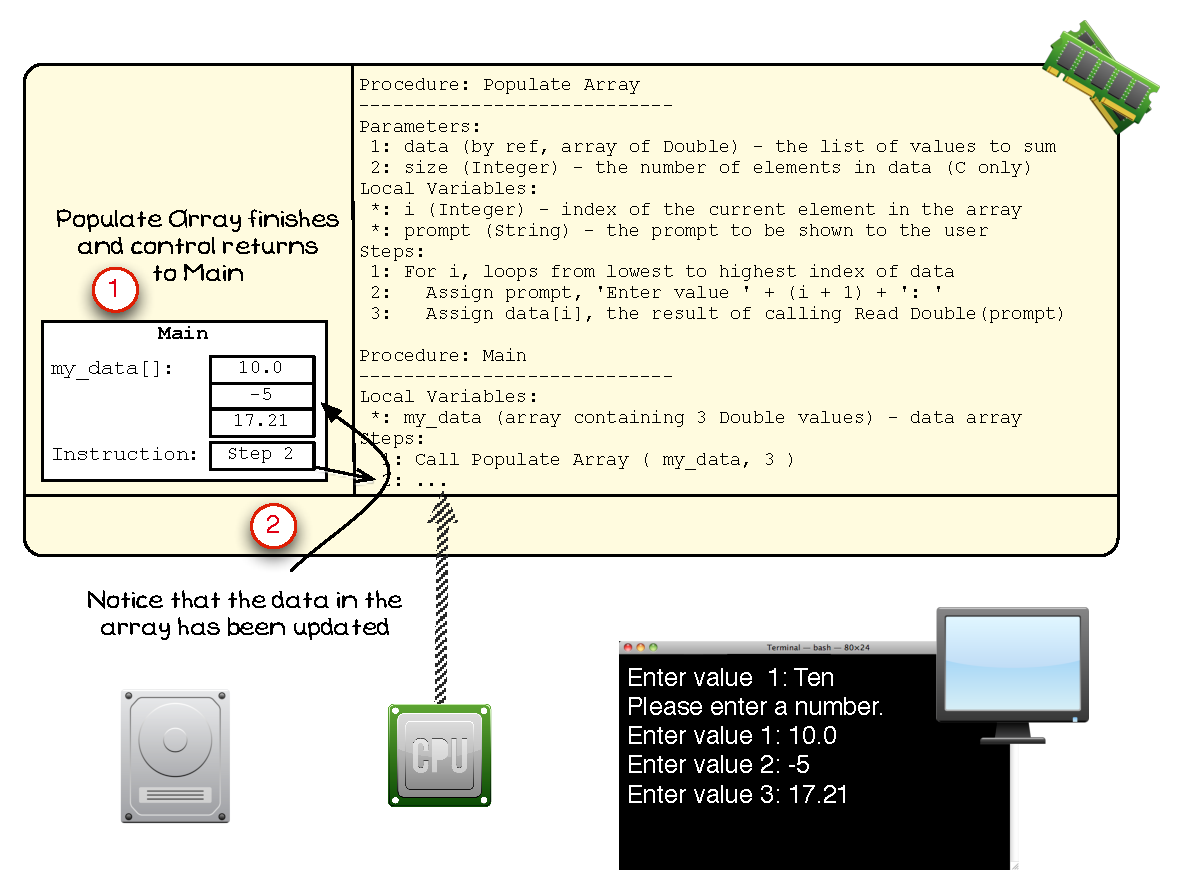
\includegraphics[width=\textwidth]{./topics/arrays/images/PopulateArray13} 
   \caption{Control returns to \texttt{Main}, and its \texttt{my\_data} array has been populated}
   \label{fig:populate-array-vis-13}
\end{figure}

\mynote{
\begin{itemize}
  \item In \fref{fig:populate-array-vis-13} the indicated areas show the following:
  \begin{enumerate}
    \item The last step in \texttt{Populate Array} has been completed, so it ends and control returns to \texttt{Main}.
    \item The values in \texttt{my\_data} have been updated. Passing this array by reference to \texttt{Populate Array} allowed it to make changes to this array's values.
  \end{enumerate}
  \medskip
  \item Notice that the data associated with the \texttt{Populate Array} procedure has been released, including the data used for the \texttt{prompt} array.
  \item \texttt{Populate Array} is responsible for filling the array passed to it with values from the user, and that is what it has done.
  
\end{itemize}
}

% subsubsection populate_array_ends_and_has_populated_main_s_my_data_array (end)
% subsection understanding_populate_array (end) 

\clearpage
\subsection{Understanding \texttt{Sum}} % (fold)
\label{sub:understanding_sum}

\fref{fig:sum-understanding} shows the flowchart of the \texttt{Sum} function from the Statistics Calculator program. This algorithm was developed in the \sref{ssub:calculating_sum}, and its Pseudocode is shown in Listing \ref{plst:sum}. The \texttt{Sum} function is responsible for calculating the sum of all of the values in the array passed to it. This is achieved by having a \texttt{total} variable that is initialised to 0, and then has the value of \emph{each element} from the array added to it.

\begin{figure}[htbp]
   \centering
   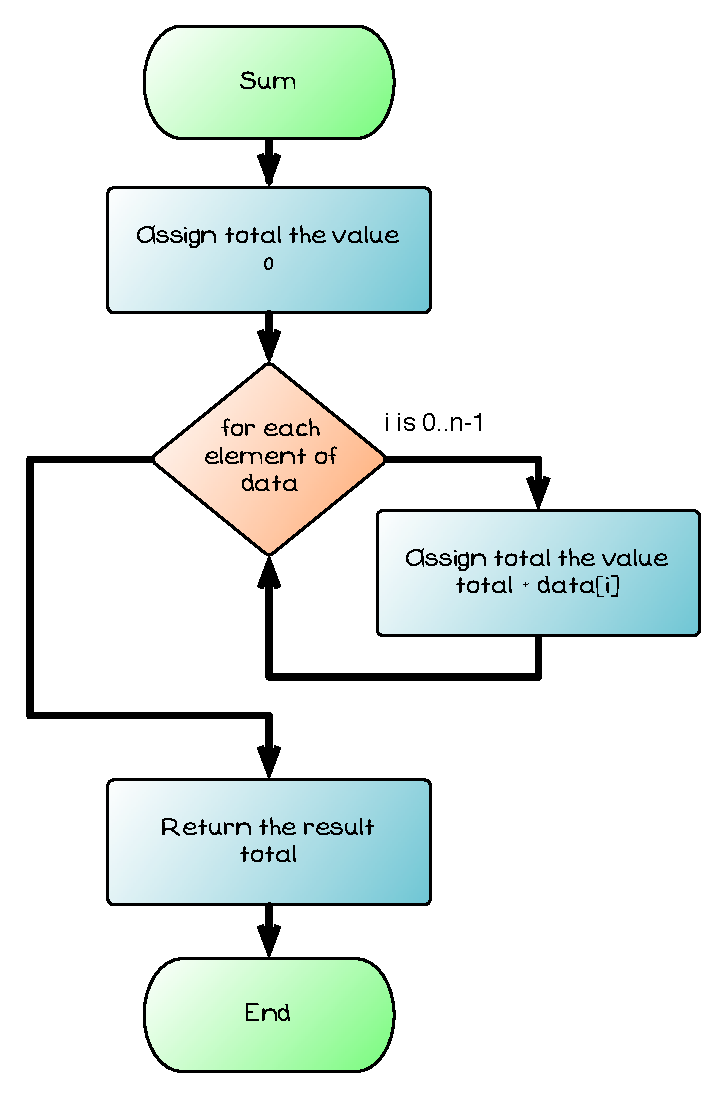
\includegraphics[width=0.5\textwidth]{./topics/arrays/diagrams/SumFlow} 
   \caption{Flowchart showing the process for \texttt{Sum}}
   \label{fig:sum-understanding}
\end{figure}

The following code will show how this function is executed on an array with three values in it. This will continue the execution from \sref{sub:understanding_populate_array} \nameref{sub:understanding_populate_array}, though the same process would occur for any array values.

\mynote{
The most important thing to pay attention to in this illustration is the interactions between the \nameref{sub:for_loop} and the \nameref{sub:array}. Make sure you can see how this combination allows you to specify the actions to be performed on an element (in the loop's body), and then to have this run for each element of the array (controlled by the loop condition).
}

\clearpage
\subsubsection{\texttt{Sum} is called, and passed the \texttt{my data} array} % (fold)
\label{ssub:sum_is_called_and_passed_the_values_in_my_data}

When \texttt{Sum} is called it is passed the array to read its values from. This is passed in the same way as was done in \texttt{Populate Array}. The difference here is that this is passed using a \texttt{const} reference, to indicate that \texttt{Sum} is not allowed to change the data in the array. This means that \texttt{Sum} will not compile if you update values in this array, and provide a guarantee to the caller that their data will not change when given to the \texttt{Sum} function. 

\begin{figure}[htbp]
   \centering
   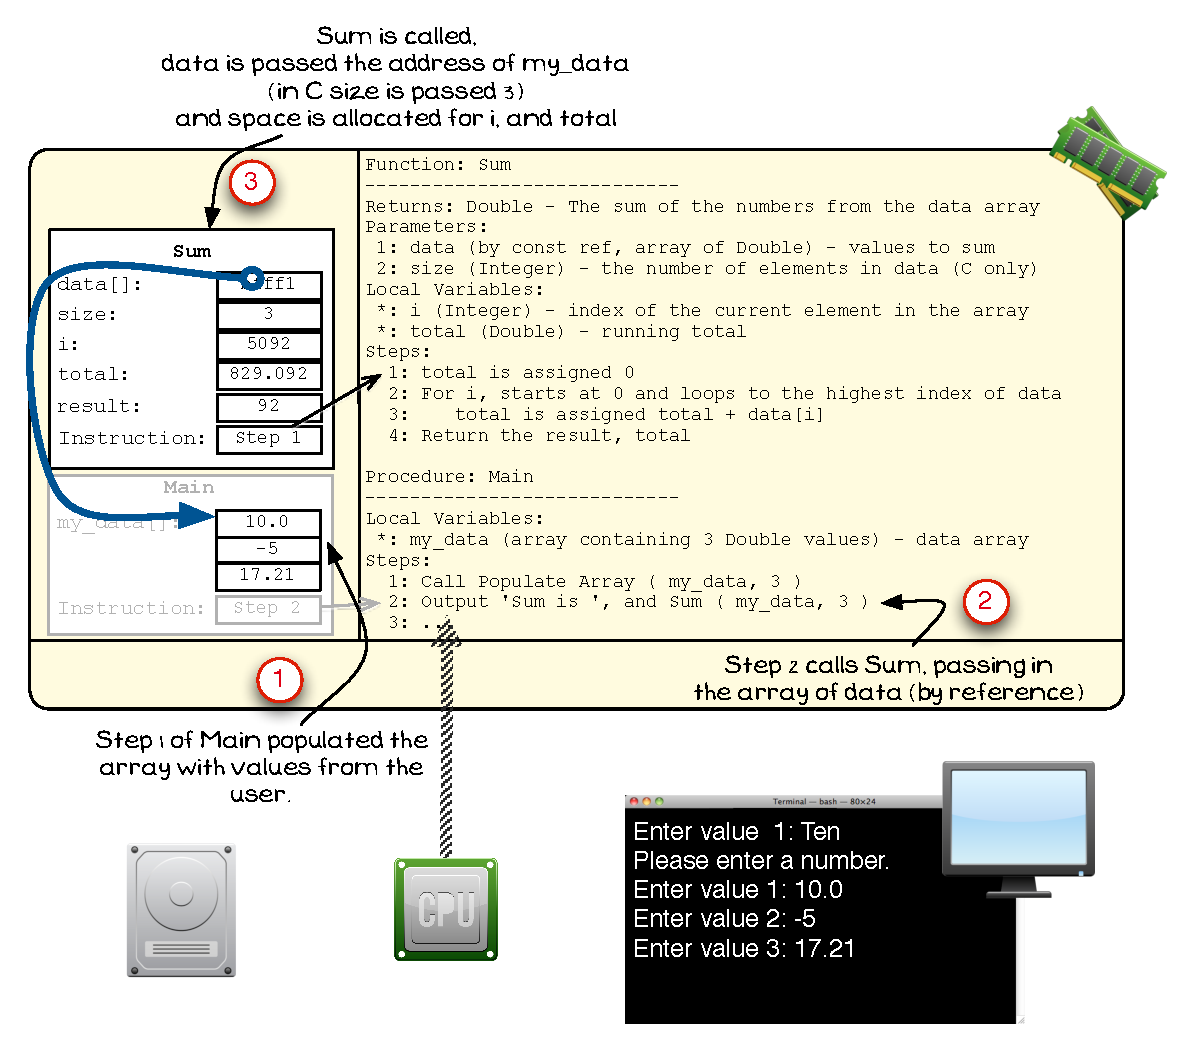
\includegraphics[width=\textwidth]{./topics/arrays/images/Sum1} 
   \caption{\texttt{Sum} is called, and it is passed the array to get its values from}
   \label{fig:sum-array-vis-1}
\end{figure}

\mynote{
\begin{itemize}
  \item In \fref{fig:sum-array-vis-1} the indicated areas show the following:
  \begin{enumerate}
    \item Step 1 of \texttt{Main} has populated the array with values.
    \item Step 2 calls the \texttt{Sum} function, passing in the \texttt{my\_data} array.
    \item When sum starts it is allocated space on the heap. Its \texttt{data} parameter is passed the address of \texttt{my\_data}. In C the \texttt{size} parameter will be passed the value 3, this isn't needed in Pascal as the language takes care of these details for you. Space is also allocated for the local variables \texttt{i} and \texttt{total}.
  \end{enumerate}
  \medskip
  \item Passing \texttt{my\_data} by reference means that sum gets a reference that \emph{points} to the start of the array.
  \item \texttt{Sum} is responsible for calculating the sum value of the values in the array.
  
\end{itemize}
}
% subsubsection sum_is_called_and_passed_the_values_in_my_data (end)

\clearpage
\subsubsection{\texttt{total} is initialised to 0} % (fold)
\label{ssub:total_is_initialised_to_0}

The first action in \texttt{Sum} is to set the value of \texttt{total} to 0. \texttt{total} will be used to store the running total of the array, and it must start at 0. Remember that the space on the stack was used before, and therefore these variables get seemingly random values initially. It is important to remember to always initialise the variables you are using.

\begin{figure}[htbp]
   \centering
   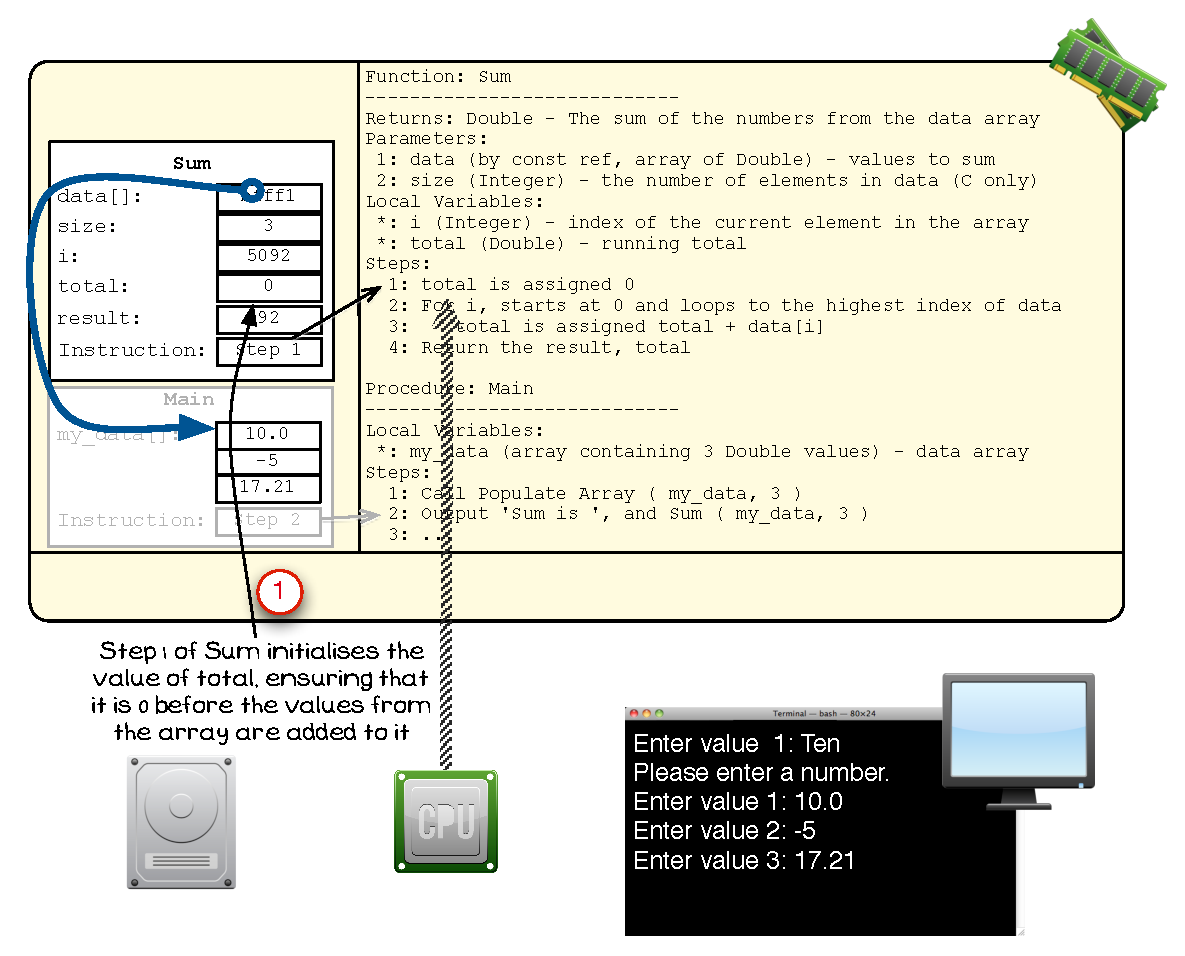
\includegraphics[width=\textwidth]{./topics/arrays/images/Sum2} 
   \caption{\texttt{Total} is initialised, having its value set to 0}
   \label{fig:sum-array-vis-2}
\end{figure}

\mynote{
\begin{itemize}
  \item In \fref{fig:sum-array-vis-2} the indicated areas show the following:
  \begin{enumerate}
    \item The \texttt{total} variable is assigned the value 0.
  \end{enumerate}
  \medskip
  \item Local variables do not get a default value when the Function or Procedure starts. You need to make sure you initialise these to appropriate values before you use them.
  \item \texttt{total} will keep a running total of the elements in the array, it must start at the value 0.
\end{itemize}
}

% subsubsection total_is_initialised_to_0 (end)

\clearpage
\subsubsection{For loop initialises \texttt{i}} % (fold)
\label{ssub:for_loop_initialises_i}

Step 2 of \texttt{Sum} starts the for loop that will iterate over the elements of the \texttt{data} array. The for loop's control variable, \texttt{i}, is set to the first index of the array and the condition checks if the loop's body should run. As \texttt{i} is in the range \texttt{0..2}, it is less than 3, control will jump into the loop's body making step 3 the next instruction.

\begin{figure}[htbp]
   \centering
   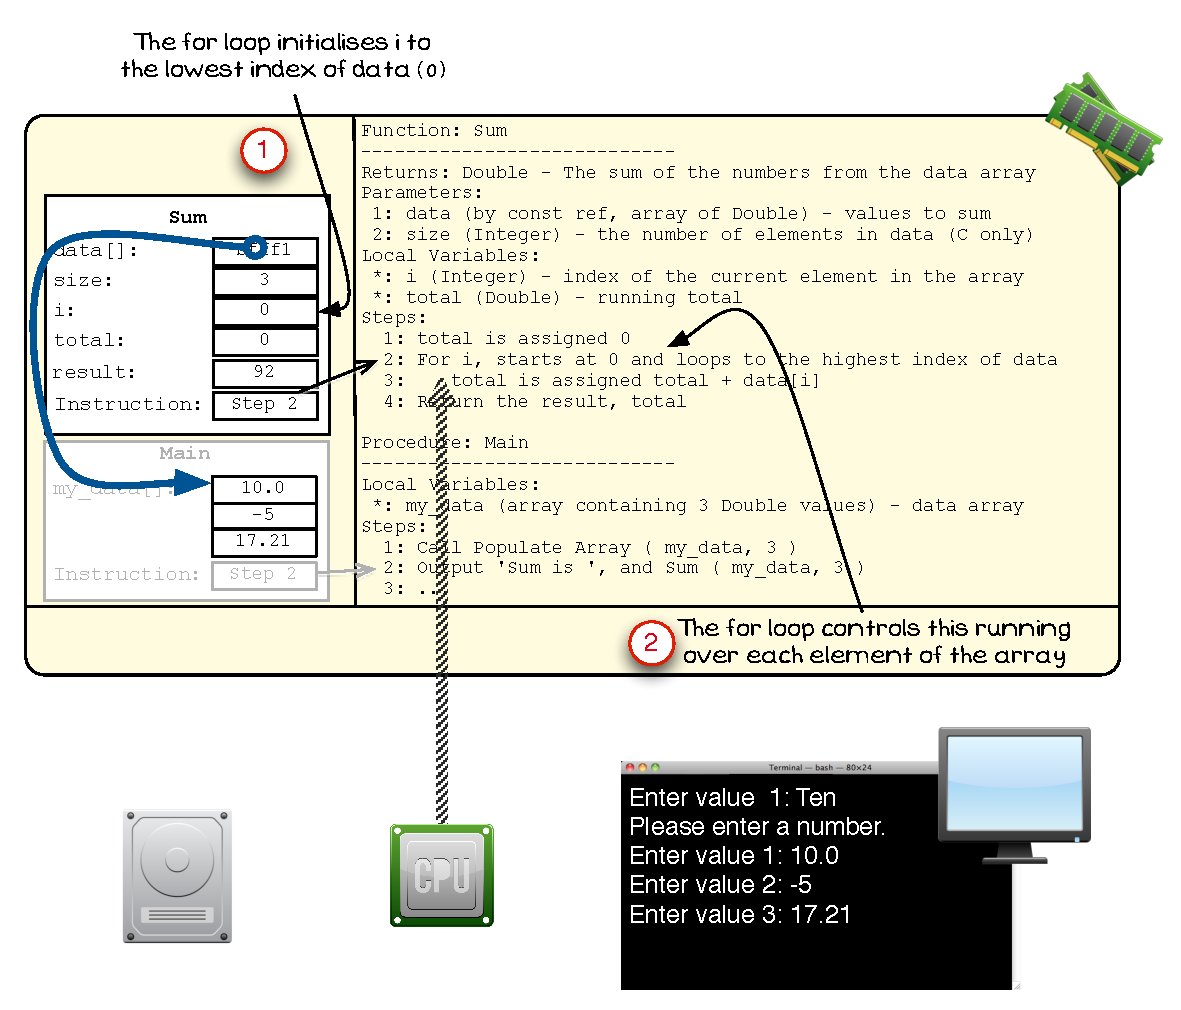
\includegraphics[width=\textwidth]{./topics/arrays/images/Sum3} 
   \caption{\texttt{i} is initialised by the for loop, and control jumps to the loop's body}
   \label{fig:sum-array-vis-3}
\end{figure}

\mynote{
\begin{itemize}
  \item In \fref{fig:sum-array-vis-3} the indicated areas show the following:
  \begin{enumerate}
    \item The for loop initialises its control variable \texttt{i}, assigning it the value 0.
    \item The condition of the loop is checked to see if the body should execute. As \texttt{i} is still in the range \texttt{0..2}, it is less than 3, the loop's body will execute.
  \end{enumerate}
  \medskip
  \item The first action of a for loop is always to initialise its control variable. After this it checks if the body of the loop should run.
\end{itemize}
}

% subsubsection for_loop_initialises_i (end)

\clearpage
\subsubsection{\texttt{total} is increased by the value in \texttt{data[0]}} % (fold)
\label{ssub:total_is_incremented_by_the_value_in_data[0]}

The body of the for loop reads the \emph{current} value from the \texttt{data} array, \texttt{data[i]}. As \texttt{i} is currently 0 this reads the first element of the array. This reads the value 10.0, which is added to the current \texttt{total}, 0. The resulting value is then stored back into the \texttt{total} variable, giving it the value 10.0, calculated from the expression \texttt{total + data[0]}, which is \texttt{0 + 10.0}.

\begin{figure}[htbp]
   \centering
   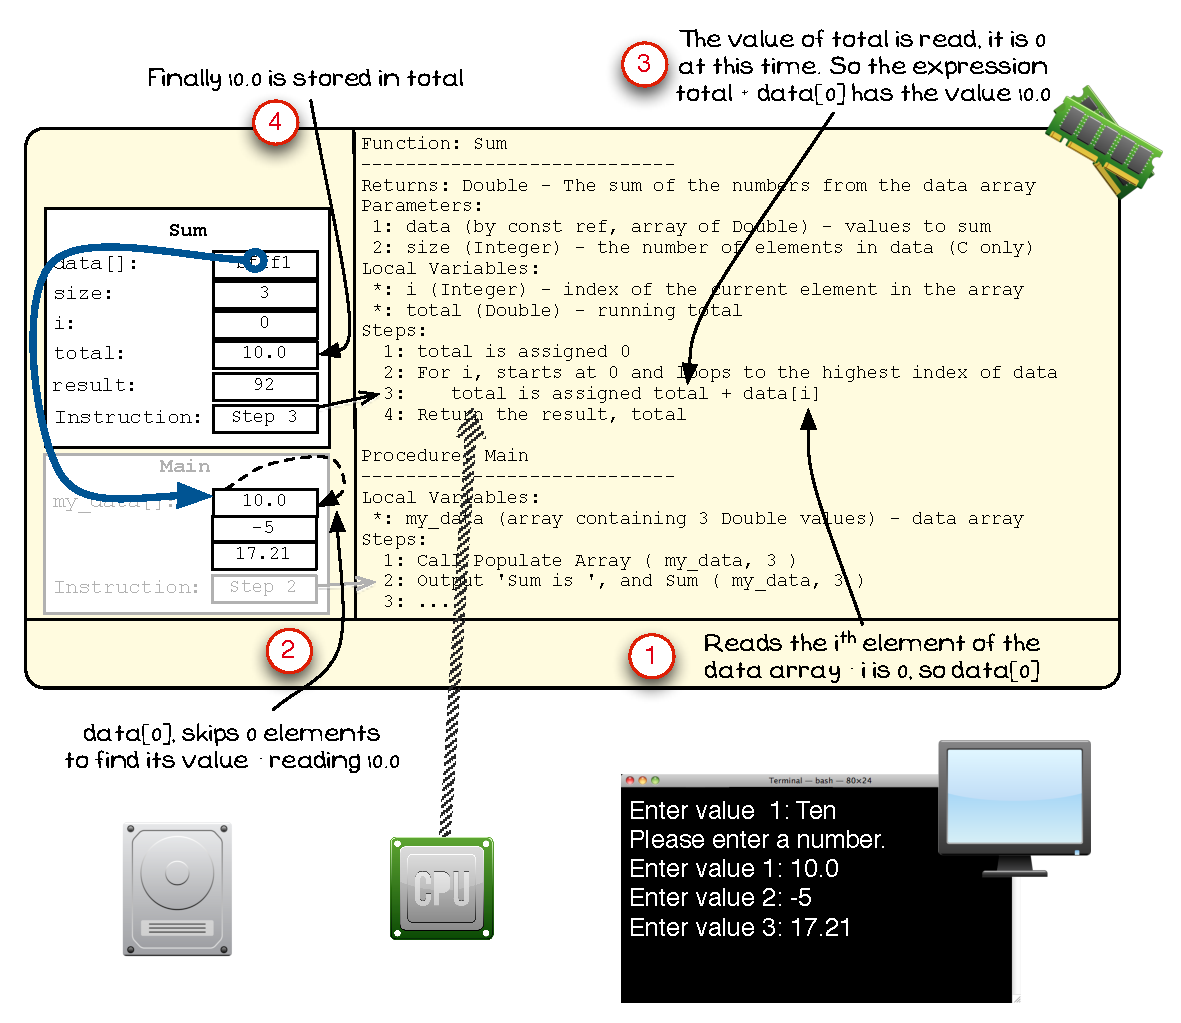
\includegraphics[width=\textwidth]{./topics/arrays/images/Sum4} 
   \caption{Total is increased by the value in \texttt{data[0]}}
   \label{fig:sum-array-vis-4}
\end{figure}

\mynote{
\begin{itemize}
  \item In \fref{fig:sum-array-vis-4} the indicated areas show the following:
  \begin{enumerate}
    \item The value of \texttt{data[i]} must be read in this expression. At this point \texttt{i} is 0, so \texttt{data[0]} must be read.
    \item \texttt{data[0]} is found in the array referred to by \texttt{data}, after skipping \texttt{0} elements. This reads the value of the first array element.
    \item The expression evaluates \texttt{total\footnote{Remember that at this point \texttt{total} has not been changed, so it has the value \texttt{0.0} as shown in \fref{fig:sum-array-vis-3}.} + data[i]}, giving \texttt{total + data[0]}, which is \texttt{0 + 10.0}, with the final value being \texttt{10.0}.
    \item The value 10.0, calculated above, is then stored in \texttt{total}.
  \end{enumerate}
  \medskip
  \item The body of the for loop provides the instructions that are run for each element of the array.
\end{itemize}
}

% subsubsection total_is_incremented_by_the_value_in_data[0] (end)

\clearpage
\subsubsection{For loop increases the value of i and runs the loop body a second time} % (fold)
\label{ssub:for_loop_increases_the_value_of_i_and_runs_the_loop_body_a_second_time}

At the end of the for loop it increments the value of its control variable, assigning \texttt{i} the value 1, and then jumps back to check its condition. As \texttt{i} is still in the range 0..2 the loop body will be run again, making step 3 the next action. 

\begin{figure}[htbp]
   \centering
   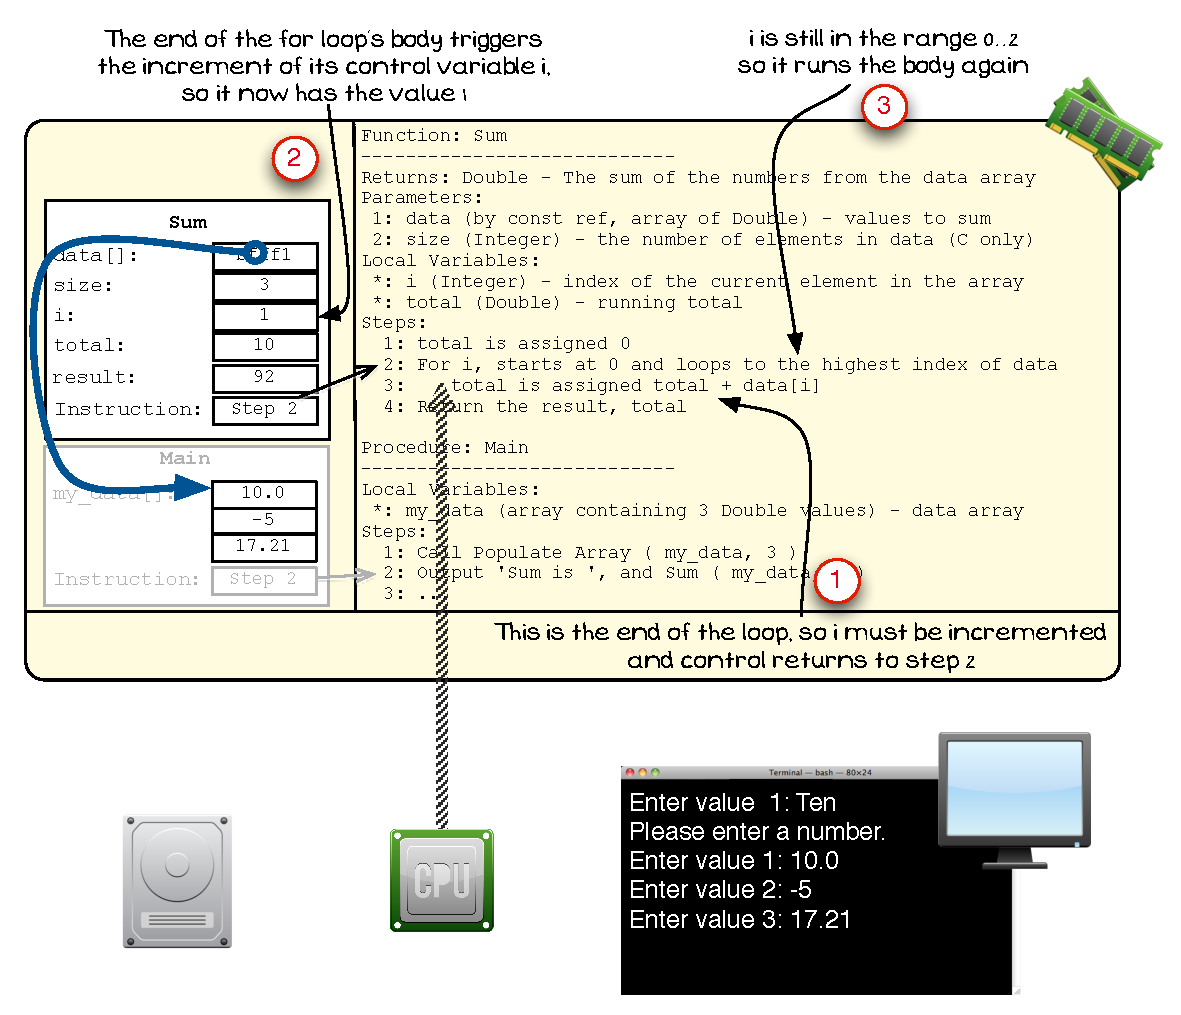
\includegraphics[width=0.95\textwidth]{./topics/arrays/images/Sum5} 
   \caption{At the end of the loop body \texttt{i} is incremented, and control jumps back to check the condition}
   \label{fig:sum-array-vis-5}
\end{figure}

\mynote{
\begin{itemize}
  \item In \fref{fig:sum-array-vis-5} the indicated areas show the following:
  \begin{enumerate}
    \item The end of the loop has been reached. The for loop increments its control variable, and jumps back to check its condition.
    \item In this case \texttt{i} is the control variable, so its value is increased to 1.
    \item The condition of the loop is checked to see if the body should execute. As \texttt{i} is still in the range \texttt{0..2} (it is less than 3) the loop's body will execute, making step 3 the next action.
  \end{enumerate}
  \medskip
  \item The end of each for loop always performs these steps. Increasing the value of its control variable, and jumping back to check its condition.
\end{itemize}
}

\csection{Remember C can do more than just counting in the for loop, though this is its main use.}


% subsubsection for_loop_increases_the_value_of_i_and_runs_the_loop_body_a_second_time (end)

\clearpage
\subsubsection{The value of \texttt{total} is increased by the value in \texttt{data[1]}} % (fold)
\label{ssub:the_value_of_total_is_increased_by_the_value_in_data[1]}

The body of the for loop reads the \emph{current} value from the \texttt{data} array, \texttt{data[i]}. Now \texttt{i} has the value 1 it reads the second element of the array. This reads the value -5, which is added to the current \texttt{total}, 10.0. The resulting value is then stored back into the \texttt{total} variable, giving it the value 5.0, calculated from the expression \texttt{total + data[1]}, which is \texttt{10.0 + -5.0}.

\begin{figure}[htbp]
   \centering
   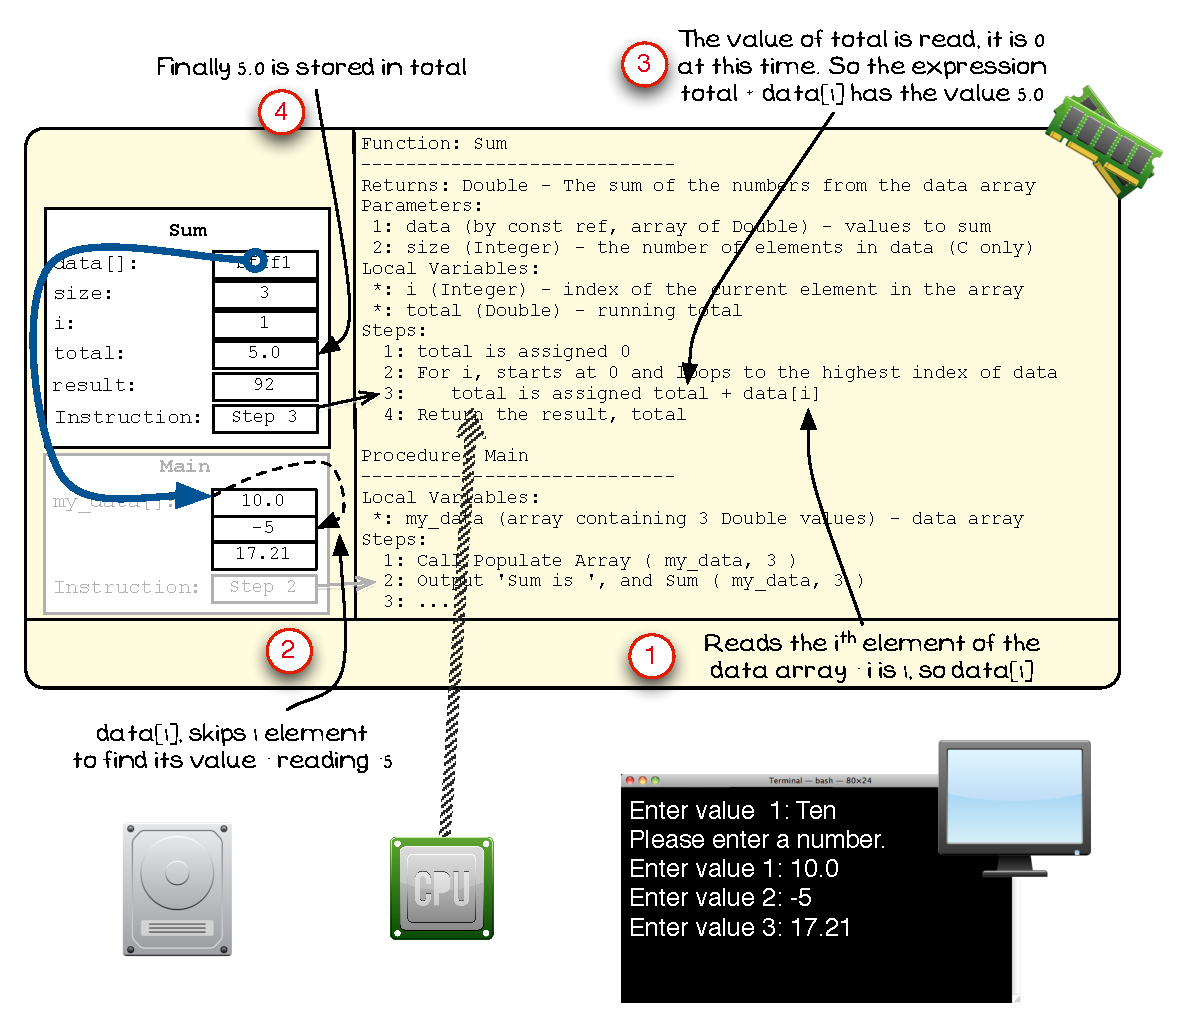
\includegraphics[width=\textwidth]{./topics/arrays/images/Sum6} 
   \caption{Total is increased by the value in \texttt{data[1]}}
   \label{fig:sum-array-vis-6}
\end{figure}

\mynote{
\begin{itemize}
  \item In \fref{fig:sum-array-vis-6} the indicated areas show the following:
  \begin{enumerate}
    \item The value of \texttt{data[i]} must be read in this expression. At this point \texttt{i} is 1, so \texttt{data[1]} must be read.
    \item \texttt{data[1]} is found in the array referred to by \texttt{data}, after skipping \texttt{1} element. This reads the value of the second array element.
    \item The expression evaluates \texttt{total\footnote{As before, \texttt{total} has not been changed at this point, so it has the value \texttt{10.0} as shown in \fref{fig:sum-array-vis-5}.} + data[i]}, giving \texttt{total + data[1]}, which is \texttt{10.0 + -5.0}, with the final value being \texttt{5.0}.
    \item The value 5.0, calculated above, is then stored in \texttt{total}.
  \end{enumerate}
  \medskip
  \item Notice that this is performing the same task, just using the next element from the array.
\end{itemize}
}

% subsubsection the_value_of_total_is_increased_by_the_value_in_data[1] (end)

\clearpage
\subsubsection{For loop increases the value of i and runs the loop body a third time} % (fold)
\label{ssub:for_loop_increases_the_value_of_i_and_runs_the_loop_body_a_third_time}

The end of the for loop has been reached again, so it increments the value of its control variable, assigning \texttt{i} the value 2, and then jumps back to check its condition. As \texttt{i} is still in the range 0..2 the loop body will run a third time, making step 3 the next action. 

\begin{figure}[htbp]
   \centering
   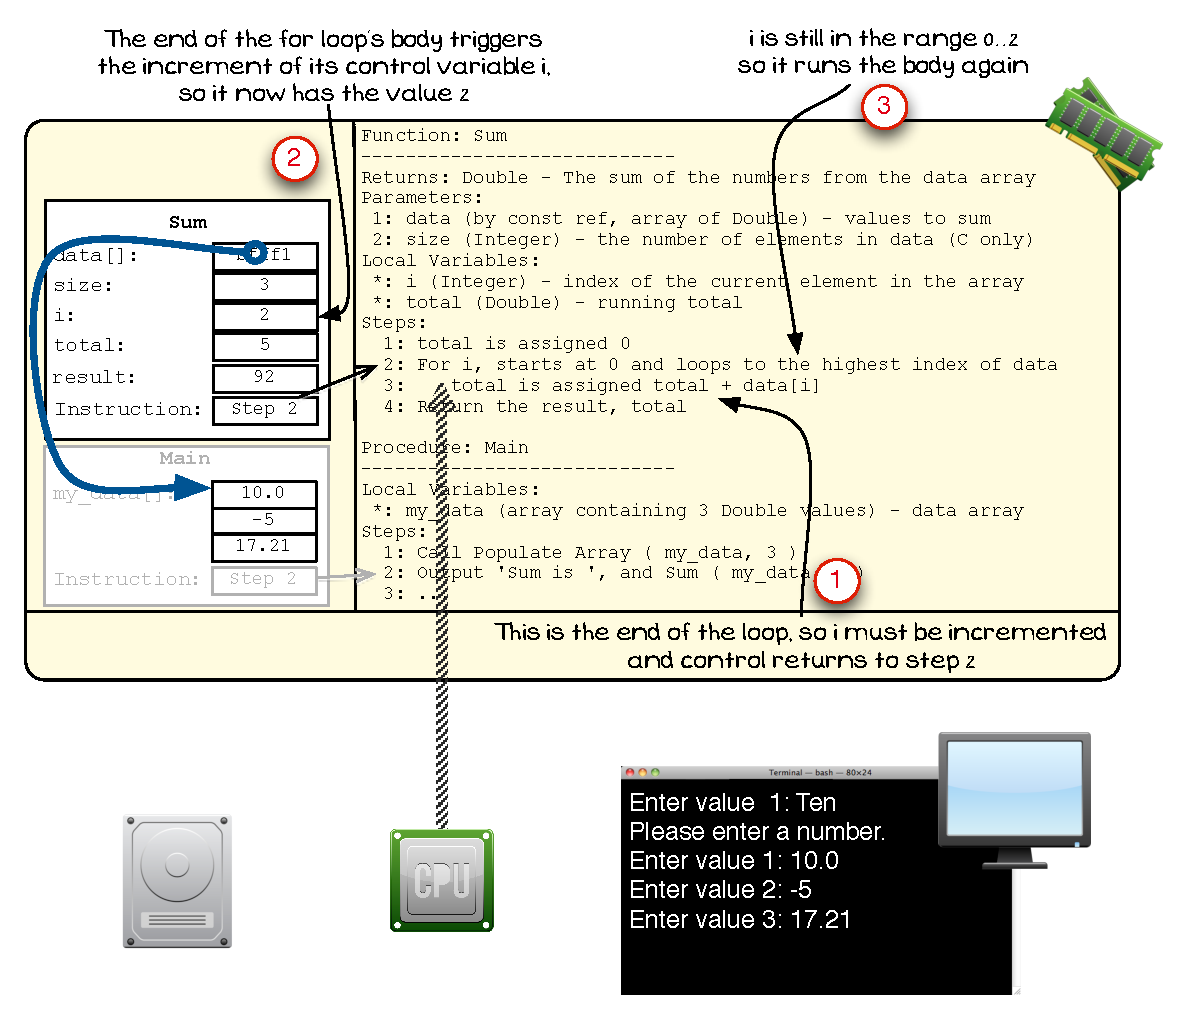
\includegraphics[width=0.95\textwidth]{./topics/arrays/images/Sum7} 
   \caption{At the end of the loop body \texttt{i} is incremented, and control jumps back to check the condition}
   \label{fig:sum-array-vis-7}
\end{figure}

\mynote{
\begin{itemize}
  \item In \fref{fig:sum-array-vis-7} the indicated areas show the following:
  \begin{enumerate}
    \item The end of the loop has been reached. The for loop increments its control variable, and jumps back to check its condition.
    \item In this case \texttt{i} is the control variable, so its value is increased to 2.
    \item The condition of the loop is checked to see if the body should execute. As \texttt{i} is still in the range \texttt{0..2} (it is less than 3) the loop's body will execute, making step 3 the next action.
  \end{enumerate}
  \medskip
  \item The end of each for loop always performs these steps. Increasing the value of its control variable, and jumping back to check its condition.
\end{itemize}
}

% subsubsection for_loop_increases_the_value_of_i_and_runs_the_loop_body_a_third_time (end)

\clearpage
\subsubsection{The value of \texttt{total} is increased by the value in \texttt{data[2]}} % (fold)
\label{ssub:the_value_of_total_is_increased_by_the_value_in_data[2]}

The body of the for loop reads the \emph{current} value from the \texttt{data} array, \texttt{data[i]}. Now \texttt{i} has the value 2 it reads the second element of the array. This reads the value 17.21, which is added to the current \texttt{total}, 5.0. The resulting value is then stored back into the \texttt{total} variable, giving it the value 22.21, calculated from the expression \texttt{total + data[2]}, which is \texttt{5.0 + 17.21}.

\begin{figure}[htbp]
   \centering
   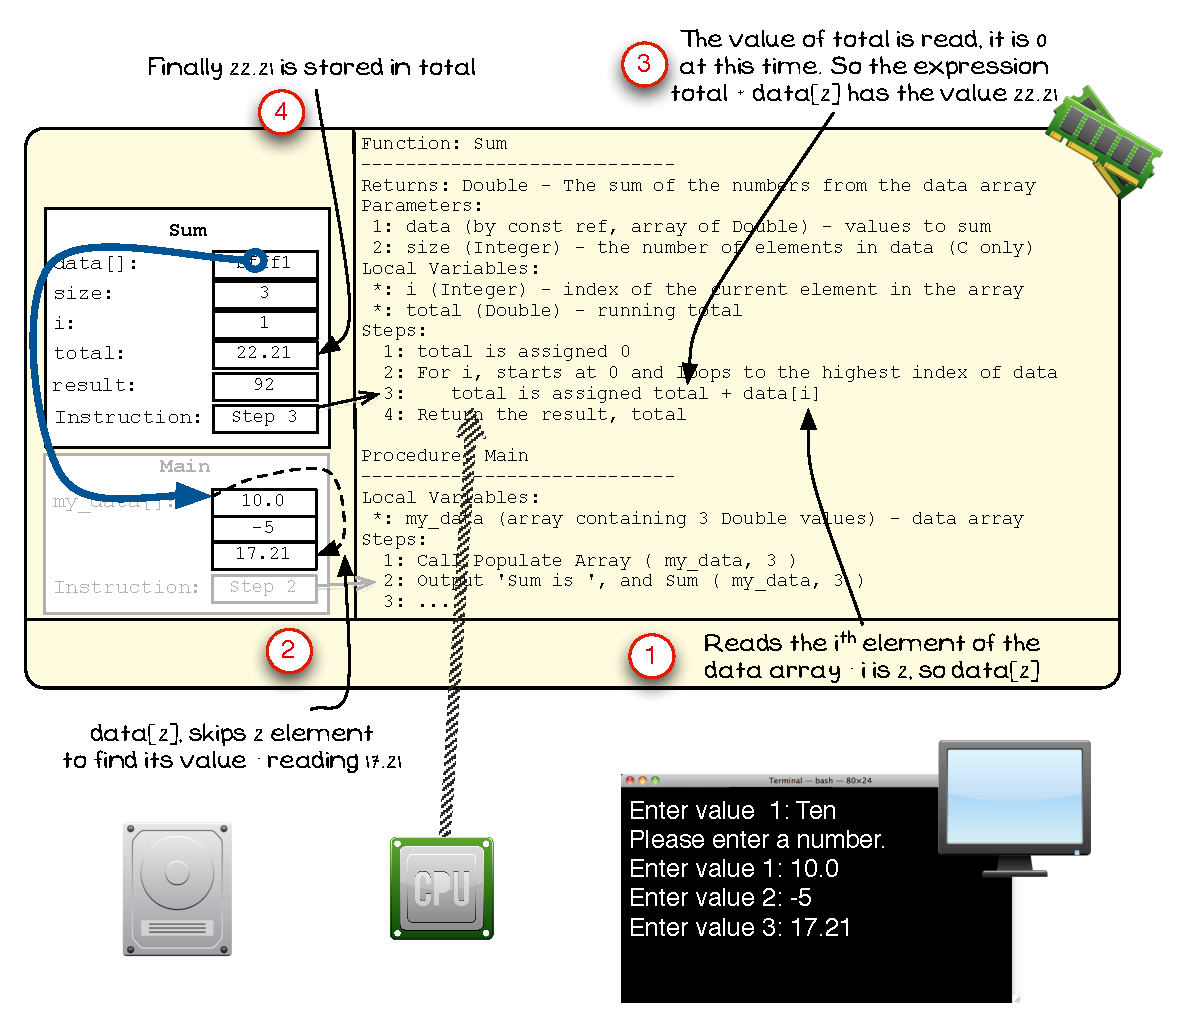
\includegraphics[width=\textwidth]{./topics/arrays/images/Sum8} 
   \caption{Total is increased by the value in \texttt{data[1]}}
   \label{fig:sum-array-vis-8}
\end{figure}

\mynote{
\begin{itemize}
  \item In \fref{fig:sum-array-vis-8} the indicated areas show the following:
  \begin{enumerate}
    \item The value of \texttt{data[i]} must be read in this expression. At this point \texttt{i} is 2, so \texttt{data[2]} must be read.
    \item \texttt{data[2]} is found in the array referred to by \texttt{data}, after skipping \texttt{2} elements. This reads the value of the third array element.
    \item The expression evaluates \texttt{total\footnote{As before, \texttt{total} has not been changed at this point, so it has the value \texttt{5.0} as shown in \fref{fig:sum-array-vis-7}.} + data[i]}, giving \texttt{total + data[2]}, which is \texttt{5.0 + 17.21}, with the final value being \texttt{22.21}.
    \item The value 5.0, calculated above, is then stored in \texttt{total}.
  \end{enumerate}
  \medskip
  \item Notice that this is performing the same task, just using the next element from the array.
\end{itemize}
}

% subsubsection the_value_of_total_is_increased_by_the_value_in_data[2] (end)

\clearpage
\subsubsection{For loop increases the value of \texttt{i}, and this time the loop finishes} % (fold)
\label{ssub:for_loop_increases_the_value_of_i_and_this_time_the_loop_finishes}

The end of the for loop has been reached again, so it increments the value of its control variable, assigning \texttt{i} the value 3, and then jumps back to check its condition. This time \texttt{i} is no longer in the range 0..2 (it is not less than 3), so the loop body will now be skipped, making step 4 the next action. 

\begin{figure}[htbp]
   \centering
   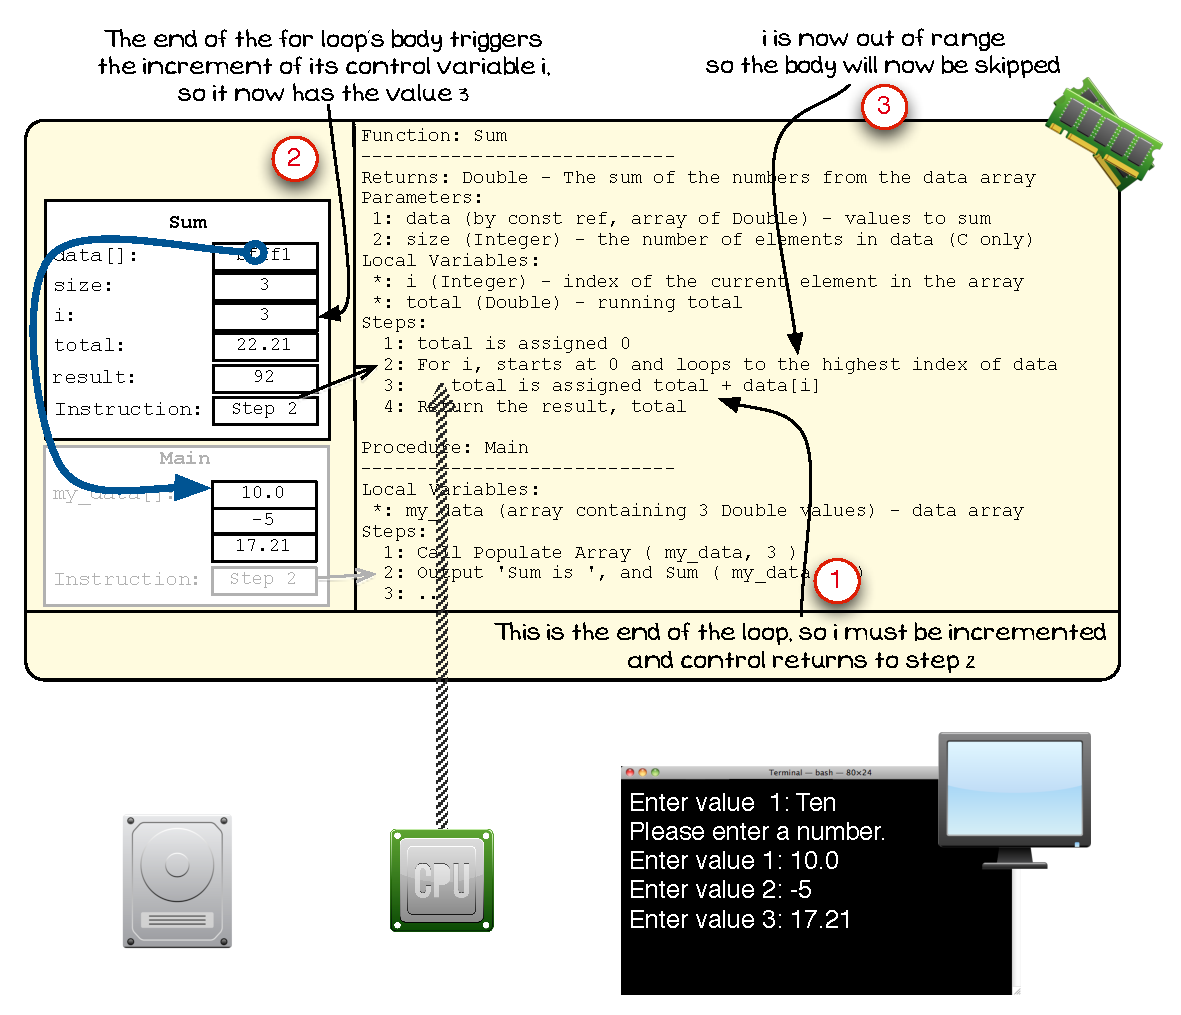
\includegraphics[width=0.95\textwidth]{./topics/arrays/images/Sum9} 
   \caption{At the end of the loop body \texttt{i} is incremented, and control jumps back to check the condition}
   \label{fig:sum-array-vis-9}
\end{figure}

\mynote{
\begin{itemize}
  \item In \fref{fig:sum-array-vis-9} the indicated areas show the following:
  \begin{enumerate}
    \item The end of the loop has been reached. The for loop increments its control variable, and jumps back to check its condition.
    \item In this case \texttt{i} is the control variable, so its value is increased to 3.
    \item The condition of the loop is checked to see if the body should execute. \texttt{i} is no longer in the range \texttt{0..2} (it is not less than 3), so the loop's body will be skipped, making step 4 the next action.
  \end{enumerate}
  \medskip
  \item The for works just like a while loop, checking its condition each loop and skipping the body when the condition is not met (when it is false).
\end{itemize}
}

% subsubsection for_loop_increases_the_value_of_i_and_this_time_the_loop_finishes (end)

\clearpage
\subsubsection{\texttt{Sum} function returns the \texttt{total} to the expression in \texttt{Main}} % (fold)
\label{ssub:sum_function_returns_the_total_to_the_expression_in_main}

The end of the for loop has been reached again, so it increments the value of its control variable, assigning \texttt{i} the value 3, and then jumps back to check its condition. This time \texttt{i} is no longer in the range 0..2 (it is not less than 3), so the loop body will now be skipped, making step 4 the next action. 

\begin{figure}[htbp]
   \centering
   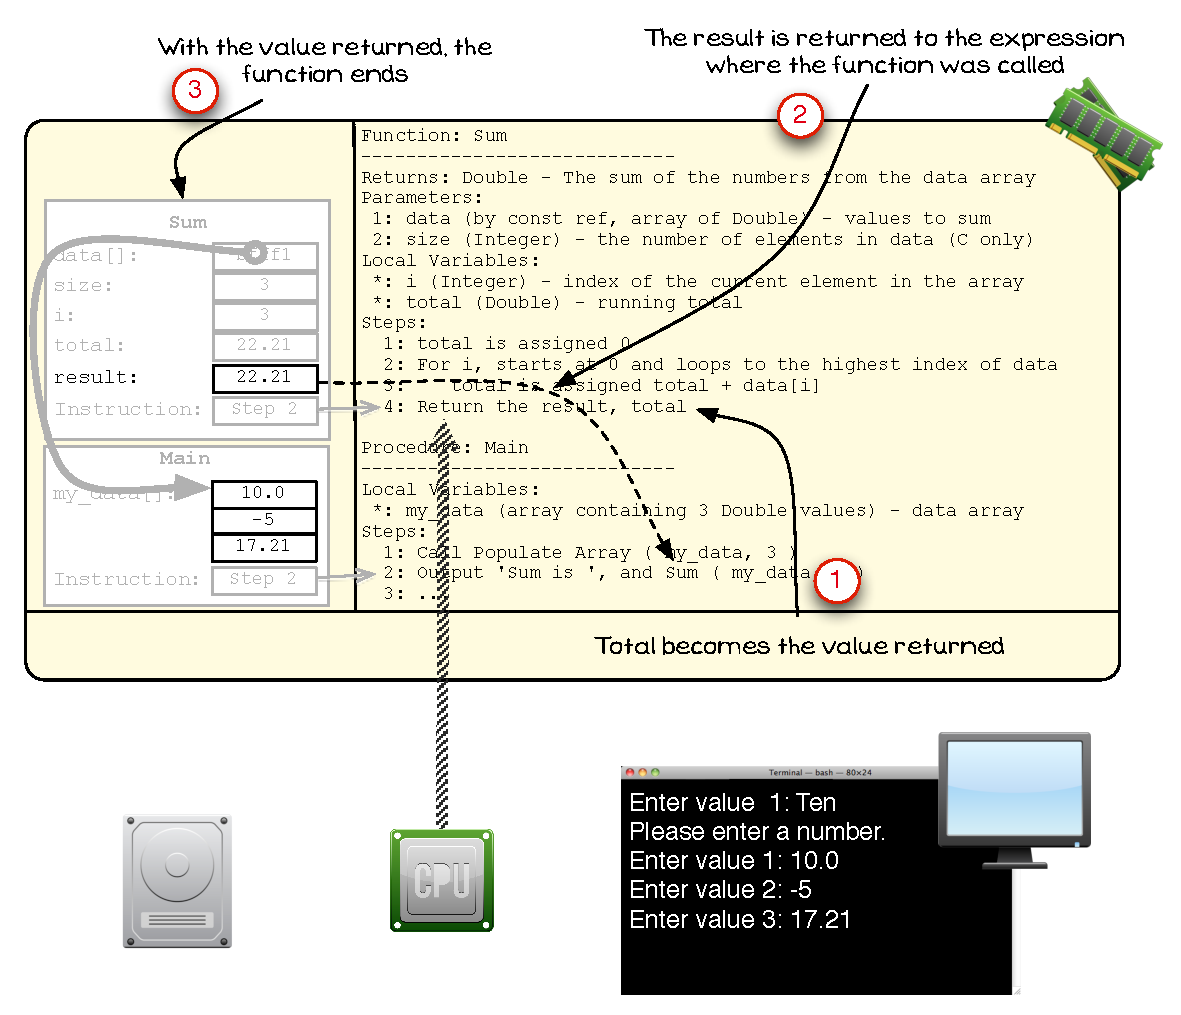
\includegraphics[width=0.95\textwidth]{./topics/arrays/images/Sum10} 
   \caption{Step 4 indicates that the value in \texttt{total} is returned to \texttt{Main}}
   \label{fig:sum-array-vis-10}
\end{figure}

\mynote{
\begin{itemize}
  \item In \fref{fig:sum-array-vis-10} the indicated areas show the following:
  \begin{enumerate}
    \item Step 4 indicates that the value in the \texttt{total} variable should be returned to the caller.
    \item The result returned by the \texttt{Sum} function is used in the expression in \texttt{Main}.
    \item As this is the end of the function its space on the stack is released, allowing control to return to \texttt{Main}.
  \end{enumerate}
  \medskip
  \item The for works just like a while loop, checking its condition each loop and skipping the body when the condition is not met (when it is false).
\end{itemize}
}

% subsubsection sum_function_returns_the_total_to_the_expression_in_main (end)

\clearpage
\subsubsection{\texttt{Main} outputs the sum to the Terminal} % (fold)
\label{ssub:main_outputs_the_sum_to_the_terminal}

\texttt{Sum} returns its value to be used in step 2 of \texttt{Main}. This step outputs the value returned to the Terminal. So by the end of Step 2 in \texttt{Main} the sum has been calculated, and written to the Terminal.

\begin{figure}[htbp]
   \centering
   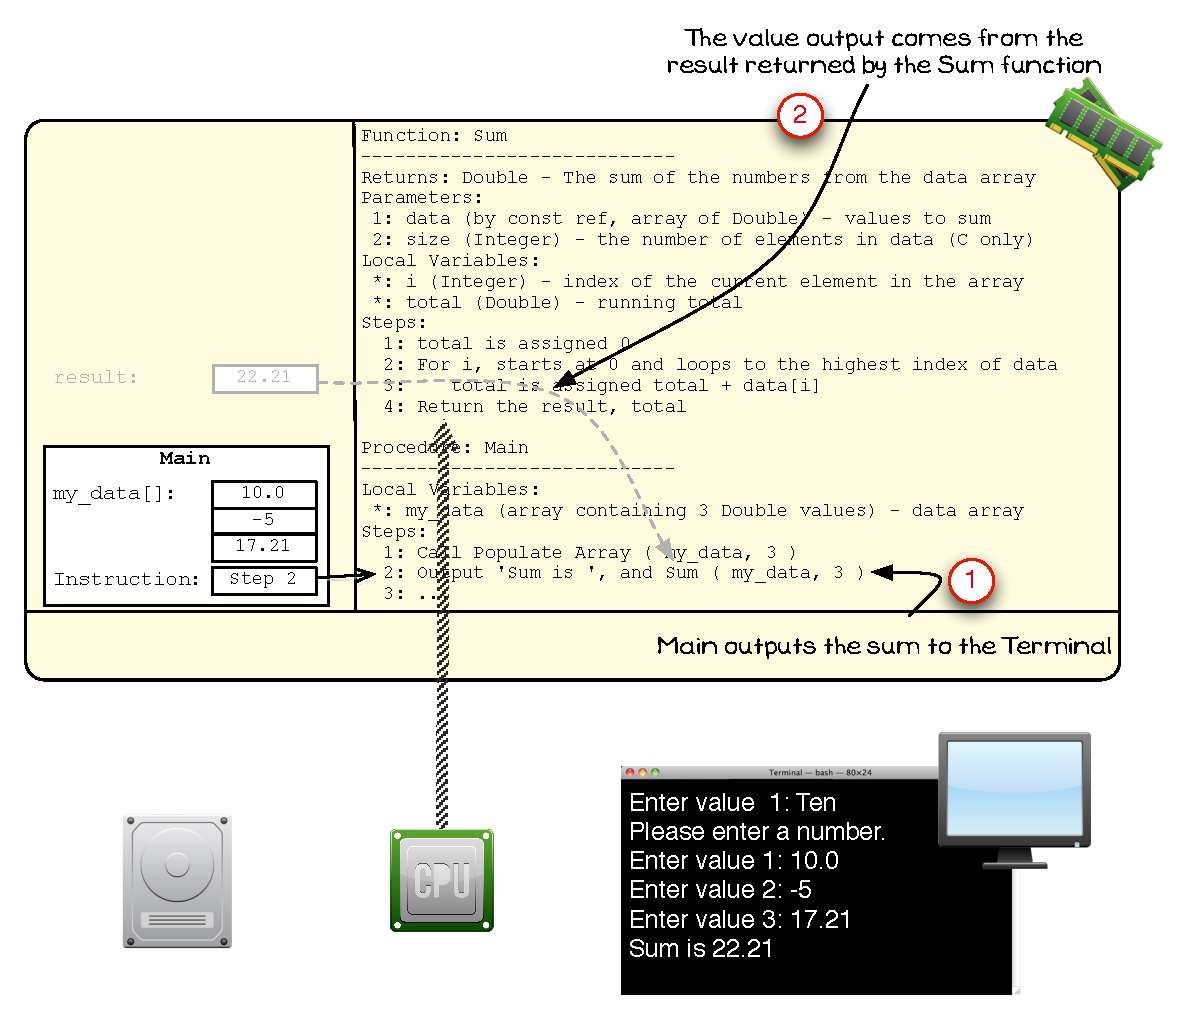
\includegraphics[width=0.95\textwidth]{./topics/arrays/images/Sum11} 
   \caption{Step 4 indicates that the value in \texttt{total} is returned to \texttt{Main}}
   \label{fig:sum-array-vis-11}
\end{figure}

\mynote{
\begin{itemize}
  \item In \fref{fig:sum-array-vis-11} the indicated areas show the following:
  \begin{enumerate}
    \item Back in \texttt{Main}, the sum is output to the Terminal.
    \item The value that is output is the value returned from the \texttt{Sum} function.
  \end{enumerate}
\end{itemize}
}

% subsubsection main_outputs_the_sum_to_the_terminal (end)

% subsection understanding_sum (end)


% section understanding_arrays (end)

% chapter more_data_types (end)